\documentclass{article}

\usepackage[utf8]{inputenc}
\usepackage{kpfonts}
\usepackage[T1]{fontenc}

\usepackage{biblatex}
\addbibresource{bibliography.bib}

\usepackage{geometry}
\geometry{a4paper, left=30mm, right=30mm, top=20mm, bottom=20mm}

\setlength{\parindent}{0em}
\setlength{\parskip}{1em}
\renewcommand{\baselinestretch}{1.5}

\makeatletter
\renewcommand\paragraph{\@startsection{paragraph}{4}{\z@}%
            {-2.5ex\@plus -1ex \@minus -.25ex}%
            {1.25ex \@plus .25ex}%
            {\normalfont\normalsize\bfseries}}
\makeatother

\usepackage{tcolorbox}
\tcbuselibrary{theorems}

\usepackage{pgfplots}
\pgfplotsset{width=\columnwidth,compat=1.13}

\usepackage{listings}
\definecolor{codegreen}{rgb}{0,0.6,0}
\definecolor{codegray}{rgb}{0.5,0.5,0.5}
\definecolor{codepurple}{rgb}{0.58,0,0.82}
\definecolor{backcolour}{rgb}{0.95,0.95,0.92}
\lstdefinestyle{mystyle}{
    backgroundcolor=\color{backcolour},   
    commentstyle=\color{codegreen},
    keywordstyle=\color{magenta},
    numberstyle=\tiny\color{codegray},
    stringstyle=\color{codepurple},
    basicstyle=\ttfamily\footnotesize,
    breakatwhitespace=false,         
    breaklines=true,                 
    captionpos=b,                    
    keepspaces=true,                 
    numbers=none,                    
    numbersep=5pt,                  
    showspaces=false,                
    showstringspaces=false,
    showtabs=false,                  
    tabsize=2
}
\lstset{style=mystyle}

\usepackage{mathtools}
\usepackage{amsthm}
\usepackage{amscd}
\usepackage{tikz-cd}

\usepackage{float}
\usepackage{titling}
\usepackage{caption}
\usepackage{subcaption}

\usepackage{hyperref}
\definecolor{maincolor}{RGB}{122, 17, 49}
\hypersetup{linkcolor=maincolor, linkbordercolor=maincolor, citebordercolor=maincolor} %colorlink removes boxes

\setcounter{section}{-1}
\setcounter{secnumdepth}{4} % how many sectioning levels to assign numbers to
\setcounter{tocdepth}{4}    % how many sectioning levels to show in ToC

\numberwithin{equation}{section}

\newtcbtheorem[number within=section]{theorem}{Theorem} {theorem style = plain, colback=maincolor!30!white, coltitle=black, colframe=white, fonttitle = \upshape\bfseries, fontupper=\itshape}{th}

\newtcbtheorem[use counter from = theorem]{definition}{Definition} {theorem style = plain, colback=maincolor!30!white, coltitle=black, colframe=white, fonttitle = \upshape\bfseries,  fontupper=\itshape}{dfn}

\newtcbtheorem[use counter from = theorem]{proposition}{Proposition} {theorem style = plain, colback=maincolor!30!white, coltitle=black, colframe=white, fonttitle = \upshape\bfseries,  fontupper=\itshape}{prop}

\newtcbtheorem[use counter from = theorem]{corollary}{Corollary} {theorem style = plain, colback=maincolor!30!white, coltitle=black, colframe=white, fonttitle = \upshape\bfseries,  fontupper=\itshape}{cor}

\newtcbtheorem[use counter from = theorem]{lemma}{Lemma} {theorem style = plain, colback=maincolor!30!white, coltitle=black, colframe=white, fonttitle = \upshape\bfseries,  fontupper=\itshape}{lemma}

\newtcbtheorem[no counter]{ob}{Observation} {theorem style = plain, colback=maincolor!30!white, coltitle=black, colframe=white, fonttitle = \upshape\bfseries,  fontupper=\itshape}{ob}

\newtcbtheorem[no counter]{conjecture}{Conjecture} {theorem style = plain, colback=maincolor!30!white, coltitle=black, colframe=white, fonttitle = \upshape\bfseries,  fontupper=\itshape}{conj}

\newtcbtheorem[no counter]{example}{Example} {theorem style = plain, colback=maincolor!10!white, coltitle=black, colframe=white, fonttitle = \upshape\itshape}{ex}

\newtcbtheorem[no counter]{technicalities}{Technicalities} {theorem style = plain, colback=maincolor!10!white, coltitle=black, colframe=white, fonttitle = \upshape\itshape}{tech}

\newtcbtheorem[no counter]{remark}{Remark} {theorem style = plain, colback=maincolor!10!white, coltitle=black, colframe=white, fonttitle = \upshape\itshape}{rem}

\DeclareMathOperator{\im}{im}
\DeclareMathOperator{\coker}{coker}
\DeclareMathOperator{\cone}{cone}
\DeclareMathOperator{\Tot}{Tot}
\DeclareMathOperator{\Hom}{Hom}
\DeclareMathOperator{\Ext}{Ext}
\DeclareMathOperator{\lExt}{\mathcal{E}\mathit{xt}} % local Ext
\DeclareMathOperator{\lHom}{\mathcal{H}\mathit{om}} % local Hom
\newcommand{\dL}{\mathbf{L}} % derived left
\newcommand{\dR}{\mathbf{R}} % derived right
\newcommand{\mL}{\mathbb{L}} % left mutation
\newcommand{\mR}{\mathbb{R}} % right mutation
\DeclareMathOperator{\RHom}{\dR Hom} % derived usual Hom
\DeclareMathOperator{\RlHom}{\dR\mathcal{H}\mathit{om}} % derived local Hom
\DeclareMathOperator{\RG}{\dR\Gamma} % derived global sections
\newcommand{\Lotimes}{\otimes^\dL} % derived tensor product
\newcommand{\lperp}[1]{\prescript{\perp}{}{#1}} % left orthogonal
\DeclareMathOperator{\Spec}{Spec}
\DeclareMathOperator{\Proj}{Proj}
\DeclareMathOperator{\Pic}{Pic}
\DeclareMathOperator{\Coh}{Coh}
\DeclareMathOperator{\QCoh}{QCoh}
\newcommand{\Ab}{\mathrm{Ab}}

% letters
\newcommand{\N}{\mathbb{N}}
\newcommand{\Z}{\mathbb{Z}}
\newcommand{\Q}{\mathbb{Q}}
\newcommand{\R}{\mathbb{R}}
\newcommand{\C}{\mathbb{C}}
\newcommand{\A}{\mathbb{A}}
\renewcommand{\P}{\mathbb{P}}
\renewcommand{\O}{\mathcal{O}}
\newcommand{\bbH}{\mathbb{H}}
\newcommand{\calH}{\mathcal{H}}
\newcommand{\calA}{\mathcal{A}}
\newcommand{\calB}{\mathcal{B}}
\newcommand{\calC}{\mathcal{C}}
\newcommand{\calD}{\mathcal{D}}
\newcommand{\calE}{\mathcal{E}}
\newcommand{\calF}{\mathcal{F}}
\newcommand{\calG}{\mathcal{G}}
\newcommand{\calL}{\mathcal{L}}
\newcommand{\calP}{\mathcal{P}}
\newcommand{\calS}{\mathcal{S}}
\newcommand{\calI}{\mathcal{I}}
\newcommand{\calN}{\mathcal{N}}
\newcommand{\calT}{\mathcal{T}}

% names
\newcommand{\id}{\mathrm{id}} % identity
\newcommand{\pt}{\mathrm{pt}} % point
\newcommand{\ev}{\mathrm{ev}} % evaluation
\newcommand{\qi}{\mathrm{q.i.}} % quasiisomorphism

\newcommand{\todo}[1]{{\color{red}\textbf{TODO!: #1}}}


\title{Derived Categories of Coherent Sheaves}
\author{Ines Chung-Halpern, Calum Crossley, Bogdan Simeonov}
\date{}

\begin{document}


\clearpage\maketitle
\thispagestyle{empty}
%\begin{figure}[H]
  %  \centering
   % \vspace{100mm}
    %\includegraphics[width=0.2\columnwidth]{kcl_logo.png}
%\end{figure}

\newpage

%\input{abstract.tex}


\newpage

\tableofcontents

\newpage

\section{Introduction}




\newpage
\section{Foundations}
When one first encounters homological algebra, for example in algebraic topology, a big emphasis is put on the homology groups of a given space. However, it turns out that these groups are not a complete invariant: there are spaces $X,Y$ such that $H_\bullet(X) \simeq H_\bullet(Y)$, but $X$ is not homotopically equivalent to $Y$. 

To remedy this, one needs a refinement of structure: instead of only considering the homology groups themselves, we can remember the whole singular chain complex $C_\bullet(X)$. Then, a theorem of Whitehead reassures us that two CW complexes with quasiisomorphic chain complexes are in fact homotopy equivalent! By enhancing homology groups to a chain level structure, homotopy equivalence becomes the same as quasiisomorphism of chain complexes. If we want to make quasiisomorphisms into an equivalence relation, however, the right object of study is the derived category. 

In this section, we cover the basic construction of the derived category and in particular many important properties of $\calD(X)$, the derived category of a variety $X$.

\subsection{The derived category of an abelian category}

Suppose we have an abelian category $\calA$: the main example we will be considering is the coherent sheaves on a projective variety $\mathrm{Coh}(X)$. We would like to study $\mathrm{Ch}(\calA)$, which is also an abelian category, but invert the class of quasiisomorphisms. The process of inverting is called \emph{localization by a localizing class.} 
\subsubsection{Localization}

Suppose we have a class $S$ of morphisms in an abelian category $\calC$ that we would like to invert. We have to be able to cancel them on the left and right for this construction to even make sense: in other words, we should always be able to replace $f:X\to Y, s:Z\to Y$ by another morphism $s':T\to X$ such that the following diagram commutes:

\begin{equation*}
    \begin{CD}
        T @>g>> Z \\
          @Vs'VV @VVsV \\
        X @>>f> Y
    \end{CD}
\end{equation*}

A class of morphisms is called a \emph{localizing class} if it satisfies this property.

\begin{definition}{Localization}{Localization}
    Suppose $\calC$ has a localizing class $S$. Then $\calC[S^{-1}]$ is the category with objects the same as that of $\calC$ and morphisms given by equivalence classes of roofs which we think of as $s^{-1}f$. Two roofs are the same if there is a bigger roof restricting to them (one can think of this as a larger numerator, or lcm)
\end{definition}

Composition is defined by choosing some roof as follows:

\[\begin{tikzcd}
    &                                    & F \arrow[ld, "s''"'] \arrow[rd, "h"] &                                     &   \\
    & D \arrow[ld, "s"'] \arrow[rd, "f"] &                                      & E \arrow[ld, "s'"'] \arrow[rd, "g"] &   \\
A \arrow[rr, "f/s", dotted] \arrow[rrrr, "g/s' \circ f/s=g\circ h/ s'\circ s''"', dotted, bend right] &                                    & B \arrow[rr, "g/s'", dotted]         &                                     & C
\end{tikzcd}\]
Under these constructions, morphisms in $S$ become invertible.

We run into the following problem: the quasiisomorphisms that we want to invert are not a localizing class in $\mathrm{Ch}(\calA)$! The way to get around this issue is to introduce the homotopy category, where they do indeed localize:

\begin{theorem}{Quasiisomorphisms localize in the homotopy category}{Quis form a localizing class}

    Quasiisomosphisms form a localizing class in the homotopy category of an abelian category $K(\calA)$\footnote[1]{This is the category where we mod out by chain homotopy equivalence, see e.g. \cite{Weibel}}. We denote the derived category by
    \begin{equation*}
        D(\calA)\coloneqq K(\calA)[Q^{-1}]
    \end{equation*}
\end{theorem}

%This is an additive category. Moreover, the cohomology functor factors through this.

Before embarking on the proof of this, let us recall the following construction from homological algebra:

\begin{definition}{Mapping cone}{Mapping cone}
    The mapping cone of $f:A^\bullet\to B^\bullet$ is the complex $A^\bullet[1]\oplus B^\bullet$ with differential $\begin{pmatrix} -d_A & 0 \\ f & d_B \end{pmatrix}$.
\end{definition}

The three objects $A^\bullet, B^\bullet, \mathrm{cone}(f)$ fit into a long exact sequence of cohomology groups. On the level of the homotopy category, we would like to put the boundary map on the same footing as the other ones, and form what is called a \emph{distinguished triangle}: \[\begin{tikzcd}
    & B^\bullet \arrow[rd] &                                       \\
A^\bullet \arrow[ru, "f"] &                      & \mathrm{cone}(f) \arrow[ll, "{[-1]}"]
\end{tikzcd}\]

The $[-1]$ operator shifts a chain complex by $1$. We see that $f$ is a quasiisomorphism iff $\cone(f)=0$. 

We will say that a triangle is \emph{distinguished} if it is equivalent to one as above. We need to show that these triangles are well-defined and can be rotated, essentially showing that the homotopy category is a triangulated category.

\begin{proposition}{}{cones}
    $\cone(B\xrightarrow\tau\cone(f))\simeq A$ in the homotopy category.
\end{proposition}

\begin{proof}
    One needs to show that the two morphisms described below are homotopy inverses, which can be done by finding explicit chain homotopies. For more details, consult \cite[\S4]{gelfand_methods_2003}
\end{proof}

%$$\begin{CD}A_{i+1}@> \begin{pmatrix}
%-f \\ 1 \\ 0
%\end{pmatrix}> > B_{{i+1}}\oplus A_{{i+1}}\oplus B_{i} @> > > A_{{i+1}} \\ @V -d_{A} VV @VV\begin{pmatrix}
%-d_{B}& 0 & 0 \\ 0 & -d_{A} & 0 \\1 & f & d_{B}
%\end{pmatrix}V @VV-d_{A}V \\ A_{i+2} @> > > B_{i+2}\oplus A_{i+2}\oplus B_{i+1}@> > > A_{i+2}\end{CD}$$

From this proposition, we see that the following diagram commutes:
\begin{equation*}
    \begin{CD}
        B @>>> \cone(f) @>>> A[-1] \\
          @V=VV @V=VV @VVV \\
        B @>>> \cone(f) @>>> \cone(\tau)
    \end{CD}
\end{equation*}

Now we can complete the proof that quasiisomorphisms form a localizing class in the homotopy category. The benefit of this is that we can replace $A\to B\to\cone(f)$ with $B\to\cone(f)\to\cone(\tau)$ and compose $\tau$ with another morphism.
\begin{proof}[Proof of Theorem 1.2]
    Recall that we wanted to show quasiisomorphisms form a localizing class, so we'd like to be able to factorize in two ways: suppose $f$ is a quasiisomorphism and $g$ is any morphism. We'd like to find $?$ such that $?\to C$ is a quasiisomorphism and the diagram commutes.
    \begin{equation*}
        \begin{CD}
            ? @> \qi>> C \\
            @VVV @VVgV \\
            A @>>f> B
        \end{CD}
    \end{equation*}
    This comes down to the following diagram:
    \begin{equation*}
        \begin{CD}
            \cone(\tau g)[-1] @>\qi>> C @>>> \cone(f) @>>> \cone(\tau g) \\
              @VVV @VgVV @V=VV @VVV \\
            \cone(\tau)[-1] @>>> B @>\tau>> \cone(f) @>>> \cone(\tau) \\
              @V\qi VV @V=VV @V=VV @VVV \\
            A @>>f> B @>>> \cone(f) @>>> A[1]
        \end{CD}
    \end{equation*}
    Since $f$ is a quasiisomorphism, we see that $\cone(f)=0$ and hence $\cone(\tau g)$ must be quasiisomorphic to $C[1]$. So we put $?=\cone(\tau g)[-1]$.
\end{proof}

\subsubsection{The quotient viewpoint}

It is natural to ask which objects in $K(\calA)$ become zero in $D(\calA)$. Such
a complex must be acyclic, since cohomology lifts to $D(\calA)$, and then the
map from the zero complex is a quasi-isomorphism so this suffices. In fact one
can view $D(\calA)$ as the quotient of $K(\calA)$ by the subcategory of acyclic
complexes.

\begin{definition}[label=defn:verdierquotient]{}{}
    If $\calC$ is a triangulated category, and $\calD$ is a triangulated
    subcategory, then the morphisms in $\calC$ whose cones can be taken to be
    objects of $\calD$ form a localizing class $\Sigma$. We then define the
    quotient $\calC/\calD\coloneqq\calC[\Sigma^{-1}]$.
\end{definition}

\begin{remark}{}
    In particular $0\to d$ becomes an isomorphism for any $d\in\calD$, since the
    cone is $d$, and so $\calD$ maps to zero in $\calC/\calD$. In fact
    $\calC/\calD$ is the universal triangulated category with this property.
\end{remark}

\subsubsection{Derived functors}

When we have either enough projectives or injectives, then we can restrict to the full subcategory of such objects (see \cite[Proposition~2.40]{Huybrechts}):

\begin{theorem}[label=thm:DfromK]{}{}
    Assume $\calA$ has enough projectives. Then
    \begin{equation*}
        K^-(\calP) \simeq D^-(\calA).
    \end{equation*}
    Dually, if there are enough injectives,
    \begin{equation*}
        K^+(\calI) \simeq D^+(\calA).
    \end{equation*}
\end{theorem}

In fact, this shows that the injective complexes provide a \emph{dg-enhancement} of the derived category. Classicaly, to compute sheaf cohomology, one replaces the sheaf by an injective resolution and then takes homology. In the derived category, we don't take homology but use the above equivalence to remember the whole resolution. In fact, any two resolutions are quasiisomorphic, so this object is well-defined.

%Suppose $F$ is an additive functor between abelian categories $\calA$, $\calB$. Then it induces a functor on the homotopy categories, by applying it termwise. If it is exact, then it sends quasiisomorphissms to quasiisomorphisms and commutes with kernels, cokernels etc.

\begin{definition}{Right derived functor}{Right derived functors}
    Suppose that $F:\calA \rightarrow \calB$ is a left exact functor between abelian categories, e.g. the pushforward functor. Then we can define $\dR F$, the right derived functor of $F$, by choosing an inverse to the equivalence on the left:
\begin{equation*}
    \begin{CD}
        D^+(\calA) @>>> D^+(\calB) \\
          @AAA @AAA \\
        K^+(\calI_A) @>F>> K^+(\calB)
    \end{CD}
\end{equation*}
Explicitly, we choose an injective resolution $A^\bullet\to I^\bullet$ and
define $\dR F(A^\bullet)\coloneqq F(I^\bullet)$. The $n$-th homology of this complex is defined to be $R^nF(A^\bullet)$.
\end{definition}

Dually, one can also define left derived functors for right exact functors by taking projective resolutions. 

\paragraph{Derived functors in geometry}

Now we specialize to $D^b(X)=D^b(\Coh(X))$. There are a plethora of geometric functors:

\begin{itemize}
    \item $\Gamma:\QCoh(X)\to\Ab$
    \item $\Hom:\QCoh(X)\times\QCoh(X)\to\Ab$
    \item Given $f:X\to Y$, have $f_*:\QCoh(X)\to\QCoh(Y)$. For $Y=\pt=\Spec\C$, pushforward is the same as taking global sections of the sheaf.
    \item $\lHom:\QCoh(X)\times\QCoh(X)\to\QCoh(X)$. Notice $\Gamma\circ\lHom=\Hom$. These are left exact.
    \item $\otimes$, $f^*$. These are right exact. Note that $f^{-1}$ is exact, but to get $f^*$ one tensors with the structure sheaf.
\end{itemize}

$\QCoh(X)$ has enough injectives, but not a lot of projectives. So we can define right derived functors. We would like to say that, since $g_*\circ f_*=(g\circ f)_*$ then the same holds for their derived versions. We run into the following issue: the pushforward does not respect injectives! We will introduce another class of sheaves, the flasque ones, to make this work. Now, pushforwards respect flasque sheaves! This is an example of what is called an adapted class:

\begin{definition}{Acyclic objects and adapted classes}{Adapted classes}
     An object is called $F$-acyclic if $R^iF(A)=0$ for $i>0$. A class of objects is adapted to $F$ if it is closed under $\oplus$, all objects in the class are $F$-acyclic and every object in $\calA$ can be embedded in an object of the class.
\end{definition}

Notice that one can throw in all $F$-acyclic objects in the adapted class, but that would cause a problem if we want the inclusion in the following theorem to hold.

\begin{theorem}{Composition of derived functors}{Composition of derived functors}
    Suppose $F:\calA\to\calB$, $G:\calB\to\calC$ are two functors such that $F(R_\calA)\subset R_\calB$, where these are adapted classes for $F$ and $G$ respectively. Then $\dR G\circ\dR F = \dR(G\circ F)$.
\end{theorem}

Since pushforwards send flasques to flasques, and flasques are an adapted class, we get what we originally wanted, i.e. $$\dR g_* \circ \dR f_* = \dR (g\circ f)_*$$

%Similarly, we can ask what happens to the pullback functor. Locally frees i.e. vector bundles should be an adapted class for $f^*$. But we don't have enough projectives, so the last condition does not make sense. We need an equivalent one: if $E^\bullet$ is acyclic complex of locally frees, we require that $f^*E^\bullet$ is still acyclic.

\begin{remark}{}{}
    Dually, one can define adapted classes for left-derived functors. The last condition is then that every object admits a surjection from an object of the class.
\end{remark}

\subsubsection{Morphisms in the derived category and derived Hom}

The morphisms between two chain complexes in $\mathrm{Ch}(\calA)$ tend to be quite big: in fact, there is an enhanced Hom-chain complex:

\begin{gather*}
    \Hom(A^\bullet, -):\mathrm{Ch}(\calA)\rightarrow \mathrm{Ch}(\mathrm{Ab})\\
    \Hom^n(A^\bullet,B^\bullet) = \prod\Hom(A^i, B^{i+n})
\end{gather*}
with differential $df=d_Bf-(-1)^nfd_A$. We see that $Z^0$ is just chain maps, whereas $B^0$ is chain homotopies, so $\calH^0$ is $\Hom_{K(\calA)}(A,B)$, i.e. morphisms up to homotopy. More generally, 
$$\begin{gathered}
    Z^i \Hom^\bullet(A^\bullet, B^\bullet)= \Hom_{\mathrm{Ch} \calA}(A^\bullet, B^\bullet[i])\\
    B^i \Hom^\bullet(A^\bullet, B^\bullet) = \text{morphisms homotopic to zero}\\
    H^i \Hom^\bullet(A^\bullet, B^\bullet)=\Hom_{\mathcal{K} \calA}(A^\bullet, B^\bullet[i])
\end{gathered}$$

If we want to compute $\RHom(A^\bullet,B^\bullet)$, we replace $B$ by a complex of injectives $I^\bullet$ (which can always be done by a method called the Cartan-Eilenberg resolution) and then compute $\Hom^\bullet(A,I)$.

\begin{proposition}{Morphisms in the derived category}{}
    $$\Ext^i(A^\bullet, B^\bullet):=H^i(\RHom^\bullet(A^\bullet,B^\bullet))\simeq \Hom_{\calD(\calA)}(A^\bullet, B^\bullet[i])$$
\end{proposition}

\begin{proof}
    Essentially, have the sequence of isomorphisms $$\Hom_{\calD \calA}(A^\bullet, I^\bullet[i])\simeq \Hom_{\mathcal{K} \calA}(A^\bullet, I^\bullet[i])\simeq H^i \Hom^\bullet(A^\bullet, I^\bullet)\simeq \Ext^i(A^\bullet, B^\bullet)$$
    We demonstrate this explicitly for $A^\bullet$ a single object concentrated in degree zero. Take an injective resolution $B^\bullet \to I^\bullet$. We see that
\begin{equation*}
    \Hom_{D(\calA)}(A,B^\bullet[i]) \simeq \Hom_{K(\calA)}(A,I^\bullet[i]).
\end{equation*}
But this is given by a morphism $f:A\to I^i$ which should be a chain map:
\begin{equation*}
    \begin{CD}
        0 @>>> A @>>> 0 \\
          @VVV @VfVV @VVV \\
        I^{i-1} @>>> I^i @>>> I^{i+1}
    \end{CD}
\end{equation*}
Hence, we can think of $f$ as a map in $\Hom^i(A, I^\bullet)$ which is closed. Moreover, it is exact precisely when it factors through $I^{i-1}$ which is the same as saying it is nullhomotopic. This shows that indeed $\Ext^i(A,B)\simeq\Hom_{D(\calA)}(A,B[i])$.
\end{proof}


%This construction is consistent with shifting by $n$. So
%\begin{gather*}
%    \Hom(A^\bullet, -):\mathrm{Ch}(\calA)\rightarrow \mathrm{Ch}(\mathrm{Ab})\\
%    \calH^n(\Hom^\bullet(A,B))
%        = \calH^0(\Hom^\bullet(A,B[n])
%        = \Hom_{K(\calA)}(A,B[n])
%\end{gather*}
%
%As a corollary, we see that
%\begin{equation*}
%    \calH^n\RHom(A,B) \simeq \Hom_{D(\calA)}(A,B[n])
%\end{equation*}
%just as we had for objects before, but now for arbitrary complexes of e.g. sheaves.



%In contrast, we show that if we only look up to homotopy, we get finite-dimensional vector spaces, the Ext groups:
%\begin{equation*}
%    \Ext_\calA^i(A,B) = \Hom_{D(\calA)}(A,B[i]).
%\end{equation*}
%To compute Ext, we need to replace $A$ by a projective resolution $P^\bullet\to A$, then Hom into $B$ and take cohomology. Equivalently, can resolve $B$ by injectives $B\to I^\bullet$, Hom from $A$ and take cohomology.

Now we focus on a geometric example. Take $E$ a quasicoherent sheaf. Then local Homs form a left exact functor $\lHom(E,-)$ and we can form its right derived functor
\begin{equation*}
    \RlHom(E,-):D^+(\QCoh(X))\to D^+(\QCoh(X))
\end{equation*}

\todo{mention how $D^*(\Coh)$ is equivalent to the subcategory in $D^*(\QCoh)$ of complexes with coherent cohomology}

Crucially, projective varieties have enough vector bundles to resolve any sheaf:

\begin{proposition}{}{}
    If $X$ is projective, then $\Coh(X)$ has enough locally frees.
\end{proposition}

The reason is that given $F$, there is $n\gg0$ such that $F(n)$ is generated by global sections. These are given by maps $\O_X\to F(n)$, and since $F$ is finite type we get a surjection $\O_X^N\to F(n)$. Can then untwist. In this case, every bounded above complex of coherent sheaves is quasiisomorphic to a bounded above complex of vector bundles. If $X$ is regular, can just take bounded. Need Hilbert syzygy theorem.

\todo{missing conclusion that this lets us derive $\lHom$ in the left argument using locally frees, and the results agree. the stuff about defining left derived functors in terms of adapted classes (e.g. locally frees for $f^*$) should probably come before this}

Now, $\lHom(E,-)$ takes injectives to flasques. From this, using \ref{th:Composition of derived functors} we see that
\begin{equation*}
    \RHom(E,-)=\RG(\RlHom(E,-))
\end{equation*}

%What about $\RlHom(E^\bullet, F^\bullet)$? Note that $\lHom(E^\bullet,-)$ is not a functor between $\QCoh$, but between homotopy categories. Need lemma:

%\begin{lemma}{}{}
%    If $E^\bullet$ or $F^\bullet$ is acyclic and $F^\bullet$ is a complex of injectives, then $\lHom(E^\bullet, F^\bullet)$ is acyclic.
%\end{lemma}

\subsubsection{Compatibilities between derived functors}

Recall: to derive $\lHom(\calF, -)$ we can resolve the second term by injectives, whereas to derive $\lHom(-,\calG)$ we can resolve the first term by vector bundles. Similarly for complexes of sheaves. For the derived tensor product $\calF^\bullet\Lotimes\calG^\bullet$ we have the same story, except need only use locally frees on either side. There are nice properties which can be checked on locally frees, and then taking complexes of locally frees e.g. associativity: $$(E^\bullet\Lotimes F^\bullet)\Lotimes G^\bullet \simeq E^\bullet\Lotimes(F^\bullet\Lotimes G)$$

 Now consider the left derived functor $\dL f^*:D^-(\Coh Y)\to D^-(\QCoh X)$. Since we have an adapted class of locally frees and pullbacks of vector bundles are vector bundles, we see that
\begin{equation*}
    \dL g^*\circ\dL f^* \simeq \dL(g\circ f)^*
\end{equation*}
%*Exercise:* blow up origin at plane, derive pull back structure sheaf at origin.

We have all sorts of other compatibilities:
\begin{gather*}
    \dL f^*(\calE^\bullet\Lotimes\calF^\bullet)
        \simeq \dL f^*\calE^\bullet\Lotimes\dL f^*\calF^\bullet \\
    \RHom(\calE^\bullet,\RlHom(\calF^\bullet,\calG^\bullet))
        \simeq \RlHom(\calE^\bullet\Lotimes\calF,\calG^\bullet) \\
    \RlHom(\calE^\bullet,\calF^\bullet)\Lotimes\calG^\bullet
        \simeq \RlHom(\calE^\bullet,\calF\Lotimes\calG^\bullet)\\
    \calE^\vee\Lotimes\calG^\bullet
        \simeq \RlHom(\calE^\bullet,\calG^\bullet), \quad
    \calE^\vee
        \simeq \RlHom(\calE,\O_X)
\end{gather*}

Also have an adjunction projection formula as usual:
\begin{gather*}
    \dR f_*\RlHom_X(\dL f^*\calE,\calF)
        \simeq \RlHom_Y(\calE,\dR f_*\calF) \\
    \RHom_X(\dL f^*\calE,\calF)
        \simeq \RHom_Y(\calE,\dR f_*\calF)
\end{gather*}
Works if $\calE$ is injective, $\calF$ locally free. The second version comes from the first one by taking global sections. Note that $\Gamma(f_*\calG)=\Gamma(\calG)$ and the same holds upon applying derived functors.

The adjunction formula is a version of the projection formula.
\begin{equation*}
    \dR f_*(\calE\Lotimes\dL f^*\calF)
        \simeq (\dR f_*\calE)\Lotimes\calF
\end{equation*}
The projection formula, as well as the other ones, usually requires that $\calF$ be locally free, but in the derived setting it works for everything, since we resolve by locally frees!

We finish off by citing the following incredibly useful fact:

\begin{theorem}{Cohomology and base change}{Cohomology and base change}
    Suppose we have a flat morphism $g:Y\to Z$ and a pullback square
    \begin{equation*}
        \begin{CD}
            W @>\tilde f>> Y \\
              @V\tilde gVV @VVgV \\
            X @>>f> Z
        \end{CD}
    \end{equation*}
    Then
    \begin{equation*}
        g^*\circ\dR f_*=\dR\tilde f_*\circ\tilde g^*.
    \end{equation*}
\end{theorem}
%Note that $g$ and hence $\tilde g$ being flat means the pullbacks are exact and
%don't need to be derived.
%The reason it is true is because it works in the usual case for injective sheaves and flat morphisms.

We can apply this to a classical example, the Poincare bundle on the elliptic curve.
\begin{example}{Poincare bundle}{}
When $Z=\Spec\C$, $W=X\times Y$ then we must have that
\begin{equation*}
    \dR p_*q^*\calE \simeq g^*\dR f_*\calE
\end{equation*}
where both $f$ and $g$ map to a point. But $\dR f_*=\RG$ in this case. The derived category of $\Spec\C$ is the category of graded vector spaces, where every object can be replaced by its cohomology with zero differential. Hence, the thing on the right is just
\begin{equation*}
    \O_Y\otimes_\C\RG(\calE)
\end{equation*}
where $\RG(\calE)$ is a graded vector space.

\end{example}

\begin{example}{Continued}{}
    So for example, when $X$ is an elliptic curve, then if $\calE=\O_X$ concentrated in degree zero, we have
\begin{equation*}
    \RG(\O_X)=H^\bullet(X,\O_X) = \C\xrightarrow{0}\C
\end{equation*}
Then $g^*\dR f_*\calE = \O_Y\xrightarrow{0}\O_Y = \O_Y\oplus\O_Y[1]$.

Now, let $E$ be an elliptic curve and fix $P_0\in E$. Then every degree zero line bundle is given by $\O_E(P-P_0)$. Hence
\begin{equation*}
    \Pic^0(E)\simeq E.
\end{equation*}
Can make universal bundle over $\calL\to\Pic^0(E)\times E$ given by $\calL\coloneqq\O_{E\times E}(\Delta-E\times P_0)$. We see that
\begin{equation*}
    \calL|_{P\times E}\simeq \O_E(P-P_0).
\end{equation*}
Now, note that
\begin{equation*}
    H^\bullet(E,\O_E(P-P_0))
        = \Ext^\bullet(\O_{P_0},\O_P)
        = \begin{cases}
            0, & P\neq P_{0} \\
            \C\oplus\C[1] & P=P_{0}
        \end{cases}
\end{equation*}
which is the skyscraper sheaf computation we did before.
Have the following diagram, to which we want to apply cohomology and base change:
\begin{equation*}
    \begin{CD}
        P\times E @>>> E\times E \\
          @VVV @VV\pi V \\
        P @>>> E
    \end{CD}
\end{equation*}
We have just seen, since pushforward to a point is global sections, that
\begin{equation*}
    \dR\pi_*\iota^*\calL = H^\bullet(E,\O_E(P-P_0))
\end{equation*}
From the cohomology and base change formula, this must be equal to $\dL\iota^*\dR\pi_*\calL$. We appeal to the fact that $\dR\pi_*\calL=\O_{P_0}[-1]$. Moreover, the ideal sheaf sequence is in particular a Koszul resolution:
\begin{equation*}
    0\to\O_E(-P_0)\to\O_E\to\O_{P_0}\to 0
\end{equation*}
This is a resolution of locally free sheaves allowing us to compute the derived restriction pullback of $\O_{P_0}$ which is exactly $\C\xrightarrow{0}\C$ if $P=P_0$ and $0$ if not equal, as expected.

% Question: why is $\dR\pi_{*}\calL=\O_{P_{0}}[-1]$? Need to ask Ed.

\end{example}

\begin{remark}{Fourier-Mukai transforms}{}
    What we have just seen is an example of a Fourier-Mukai kernel: the universal line bundle $\calL$ on $E\times E$, which defines an endomorphism $\Phi_\calL:D^b(E)\to D^b(E)$, $\calF\mapsto\dR p_*(q^*\calF\Lotimes\calL)$.
\end{remark}

From now on we will drop the $\dR$'s and $\dL$'s unless needed for clarity.

\subsubsection{Computing derived functors: the Grothendieck spectral sequence}

Suppose we know the approximations $R^iF(A^p)$ or $R^iF(\calH^pA)$ for a complex $A^\bullet$. How can we compute $R^iF(A)$ from this information?

We first need the Cartan-Eilenberg complex $I^{\bullet, \bullet}$, which is a special bicomplex resolution of $A^\bullet$.

One can check that $\Tot I \to A$ is a quasi-isomorphism. So $\dR F(A)=F(\Tot I)=\Tot FI$. When we take cohomology, we are interested in the $n$-th cohomology of the total complex, for which we have two spectral sequences associated to the bicomplex: one starts with horizontal differential, and the other with the vertical.

If we start with vertical, then the first page is
\begin{equation*}
    E_1^{p,q} = R^qF(A^p) \Rightarrow R^nF(A)
\end{equation*}
since we are computing derived functors of $F$. If we start with horizontal, then
\begin{equation*}
    E_2^{p,q} = R^qF(\calH^pA) \Rightarrow R^nF(A)
\end{equation*}
More generally, there is a computational tool called the \emph{Grothendieck spectral sequence} which computes the derived functors of a composition: $$E_2^{pq}=R^pG \circ R^q F\implies R^{p+q}G\circ F$$

Now we describe two very important instance of the Grothendieck spectral sequence, the Leray spectral sequence and the local to global spectral sequence.

\begin{example}{Leray spectral sequence}{} Consider a composition $X\xrightarrow{g}Y\xrightarrow{f}Z$. The Leray spectral sequence is as follows:
\begin{equation*}
    R^n(f\circ g)_*\calF
        = \calH^n(\dR(f\circ g)_*\calF)
        = \calH^n(\dR f_*\dR g_*\calF)
        = R^nf_*(\dR g_*\calF)
\end{equation*}
We are in the situation of trying to compute the n-th derived functor of $F=f_*$ of some complex $A=\dR g_*\calF$. We can apply the second spectral sequence to see that
\begin{equation*}
    E_2^{p,q}
        = R^qf_*(R^pg_*\calF)
        \Rightarrow R^n(f\circ g)_*\calF
\end{equation*}
When we apply this to $Z=\Spec\C$, then $f_*$ is global sections and $\dR f_*$ is sheaf cohomology, as is $\dR(f\circ g)_*$ which gives us the Leray spectral sequence:
\begin{equation*}
    H^q(Y,R^pg_*\calF) \Rightarrow H^{p+q}(X,\calF)
\end{equation*}
\end{example}

\begin{example}{Local to global spectral sequence}{}
We know from before that
\begin{equation*}
    \RG\circ\RlHom = \RHom
\end{equation*}
Upon taking cohomology, on the right hand side we get $\Ext^n(\calF,\calG)$. On the other hand, taking $F=\Gamma$, $A=\RlHom(\calF,\calG)$ then the spectral sequence gives us
\begin{equation*}
    H^q(X,\lExt^p(\calF,\calG)) \Rightarrow \Ext^n(\calF,\calG)
\end{equation*}
\end{example}

As an application, we compute the Ext groups of a point, as well as the self local Exts of a subvariety.

More precisely, let $Y\subset X$ be a subvariety given by the zero locus of a section of $\calE$, which we can Koszul resolve:
\begin{equation*}
    \cdots\to\wedge^2\calE^\vee\to\calE^\vee\to\O_X\to\O_{Y}\to0
\end{equation*}
i.e. we replace $\O_Y$ by $\bigwedge^\bullet\calE^\vee$. Then $\lExt^\bullet(\O_Y,\O_Y)$ is computed by applying $\lHom(-,\O_Y)$ to the complex and taking cohomology. But once we restrict to $Y$, the maps become zero since they are given by the defining section $s$ for $Y$. Hence, the complex is formal and we get
\begin{equation*}
    \lExt^i(\O_Y,\O_Y)
        = \lHom(\bigwedge\nolimits^i\calE^\vee,\O_Y)
        = \bigwedge\nolimits^i\calE\otimes\O_Y
        = \bigwedge\nolimits^i\calE|_Y
        = \bigwedge\nolimits^i\calN_{Y/X}
\end{equation*}
This allows us to compute the self Ext groups of a point, by using the local-to-global spectral sequence:
\begin{equation*}
    H^i(X,\lExt^j(\O_p,\O_p)) \Rightarrow \Ext^{i+j}(\O_p,\O_p)
\end{equation*}
The local homs will be supported at $p$. So it has no higher cohomology i.e. the cases $i>0$ give nothing. But when $i=0$, we have no differential. So in fact
\begin{equation*}
    \Ext^\bullet(\O_p,\O_p) \simeq H^0(X,\lExt^\bullet(\O_p,\O_p))
\end{equation*}
From the Koszul resolution, we see that the latter is just an exterior algebra!

\begin{remark}{Deformations}{}
    We see that the global sections of the normal bundle of $Y$, which describe its deformations inside $X$, can be described by $\Ext^1(\O_Y,\O_Y)$.
\end{remark}
We mention briefly the Hochschild cohomology $HH^\bullet(X):=\Ext^\bullet(\O_{\Delta_X}, \O_{\Delta_X})$ in the form of the following important theorem, which boils down to the local-to-global spectral sequence degenerating:
\begin{theorem}{Hochschild-Kostant-Rosenberg}{HKR}
    $$HH^k(\mathcal{D}(X))=\bigoplus_{p+q=k} H^q(X, \Lambda^p T_X), HH_k(\mathcal{D}(X))=\bigoplus_{q-p=k} H^q(X, \Omega^p_X)=\bigoplus_{q-p=k} H^{p,q}(X)$$
    
\end{theorem}

\begin{remark}{Mirror symmetry}{}
    In mirror symmetry, varieties come in pairs such that the Floer cohomology groups on one side correspond to Ext groups on the other. If we think of $X$ as the moduli space of its skyscraper sheaves, then since Ext groups should match up with self Floer groups, the mirrors to points should be Lagrangians with self Floer cohomology equal to an exterior algebra. But self Floer cohomology is equal to usual cohomology for unobstructed Lagrangians, which motivates the fact that mirror to points we should have (special) Lagrangian tori. This is the basis of the SYZ philosophy.
\end{remark}

\subsection{Serre duality}

Serre duality is a classical fact about projective varieties that can be lifted to a structure on the derived category. We explain how.

\begin{proposition}{Classical Serre duality}{Classical Serre duality}
    If $X$ is smooth projective over $\C$, and $\calE$ is a vector bundle on $X$, then
    \begin{equation*}
        H^i(X,\calE)^* \simeq H^{n-i}(X,\calE^\vee\otimes\omega_X)
    \end{equation*}
\end{proposition}

The duality is given by a pairing. Namely, we have a perfect pairing
\begin{equation*}
    H^i(X,\calE)\otimes H^{n-i}(X,\calE^\vee\otimes\omega_X)
        \to H^n(X,\calE\otimes\calE^\vee\otimes\omega_X)
        \xrightarrow{\mathrm{tr}} H^n(X,\omega_X)
        \xrightarrow{\simeq} \C 
\end{equation*}
An alternative way to prove this is via the Hodge star operator on vector bundles.

There is also a hypercohomology version. If we replace $\calE$ by a complex of vector bundles, we define the dual complex as
\begin{equation*}
    \lHom(\calE^\bullet,\O_X)^n = \lHom(\calE^{-n},\O_X)
\end{equation*}
Similarly, there is a trace map $\calE^\vee\otimes\calE\to\O_X$, so in the same way we can construct a pairing.

%*Example:* $\calE=V^0\to W^1$. The dual complex is $W^\vee\to V^\vee$, where now $W^\vee$ lives in degree $-1$. The tensor complex is $$W^\vee \otimes V \to  V^\vee \otimes V \oplus W^\vee \otimes W \to  V^\vee \otimes W$$The map is the natural one in degree zero.

\begin{proposition}{Serre duality for complexes}{Serre duality for complexes}
    Define the hypercohomology of a complex as $\bbH^i(X,\calE)\coloneqq\calH^i\RG(\calE)$. Then
    \begin{equation*}
        \bbH^i(X,\calE)\otimes\bbH^{n-i}(X,\calE^\vee\otimes\omega_X)\to\C
    \end{equation*}
    This pairing is still perfect.
\end{proposition}

One can use the LES on hypercohomology via truncating complexes and reduce this to the case of vector bundles (this method of proof is called devissage).

Finally, we come to the categorical version:

\begin{proposition}{Categorical form of Serre duality}{Categorical form of Serre duality}
    If $A,B\in D^b(X)$, and $n=\dim X$, then
    \begin{equation*}
        \Hom(A,B)^\vee \simeq \Hom(B,A\otimes\omega_X[n])
    \end{equation*}
\end{proposition}

The idea is as follows: we can compute the Homs of the derived category as
\begin{align*}
    \Hom_{\calD^b(X)}(B,A\otimes\omega_X[n])
        &\simeq \calH^n\RHom(B,A\otimes\omega_X) \\
        &\simeq \calH^n\RG(\RlHom(B,A\otimes\omega_X)) \\
        &\simeq \bbH^n(X,B^\vee\Lotimes A\otimes\omega_X).
\end{align*}

Similarly,
\begin{align*}
    \Hom_{\calD^b(X)}(A,B)
        &\simeq \calH^0\RHom(A,B) \\
        &\simeq \calH^0\RG(X,\RlHom(A,B)) \\
        &\simeq \bbH^0(X,A^\vee\Lotimes B).
\end{align*}
These are dual by the previous version of Serre duality, applying it to $\calE=A^\vee\Lotimes B$.

\begin{definition}{Serre functor}{Serre functor}
    Define $S:D^b(X)\to D^b(X)$, $F\mapsto F\otimes\omega_X[\dim X]$. Then
    \begin{equation*}
        \Hom(A,B)^*\simeq\Hom(B,S(A))
    \end{equation*}
     A Serre functor is an additive, $\C$-linear autoequivalence obeying the above property. 
\end{definition}

Two such functors are canonically equivalent, since $S(A)$ represents the functor $B\mapsto\Hom(A,B)^*$.

% Check that $S$ commutes with any autoequivalence: $$\begin{gathered}
% \Hom(B,SFA)\simeq \Hom(FA,B)^*\\
% \Hom(B,FSA)\simeq \Hom(F^{-1}B,SA)\simeq \Hom(A, F^{-1}B)^*\simeq \Hom(FA,B)^*
% \end{gathered}$$So the two represent the same functor.

% The element $1_A$ corresponds via the isomorphism to some $\tau_A: \Hom(A, S(A))\to k$, which we call a trace.

% *Exercise:* given sequence $$A\xrightarrow{x}B\xrightarrow{y}S(A)\xrightarrow{S(x)}S(B)$$then $\mathrm{Tr}(yx)=\mathrm{Tr}(S(x)y)$.

The Serre functor allows us to switch between left and right adjoints. Suppose $F$ left adjoint to $G$. Then $SFS^{-1}$ is right adjoint to $G$.

% The point is that the duality pairing is the same as the composition and then the trace: $\mathrm{Tr}(y\circ x)=\mu(x,y)$, where $\mu$ is the duality pairing. Claim we have a commutative diagram, where on the left we send $(x,y)\mapsto(y, Sx)$.
% $$\begin{CD}
% \Hom(A,B)\otimes \Hom(B,SA)@> > > k\\ @VVV @VVV \\ \Hom(B,SA)\otimes \Hom(SA,SB)@> > > k
% \end{CD}$$
% Equivalently, can think about composite isomorphisms $$\Hom(B,SA)\simeq \Hom(A,B)^*\simeq \Hom(SA,SB)^*\simeq \Hom(B,SA)$$
% The first arrow sends $x\mapsto \mu(x,-)$. However, the leftmost arrow is given by $x\mapsto \mu(-,x)$. Hence, the two are related via $S$ and so $\mathrm{Tr}(yx)=\mu(x,y)=\mu(y,Sx)=\mathrm{Tr}(S(x)y)$.

\begin{definition}{Calabi-Yau category}{Calabi-Yau category}
    A category is called a Calabi-Yau $n$ category if it has a Serre functor given by just shifting by $n$, $S=[n]$.
\end{definition}

\begin{example}{Shriek functor and Grothendieck-Verdier duality}{Shriek functor}
Given $f:X\to Y$, we have that $\dL f^*$ is left adjoint to $\dR f_*$. In both categories there are Serre functors, so can obtain the right adjoint to the pushforward as
\begin{gather*}
    f^!(A) \coloneqq (\dL f^*A\otimes f^*\omega_Y^{-1}[-\dim Y])
            \otimes \omega_X[\dim X] \\
        = \dL f^*A\otimes(f^*\omega_Y^{-1}\otimes\omega_X)[\dim X -\dim Y]
\end{gather*}
We call $\omega_f\coloneqq f^*\omega_Y^{-1}\otimes\omega_X=f^!\O_Y$, the relative dualizing sheaf. The adjunction reads
\begin{equation*}
    \Hom(\dR f_*A,B)\simeq \Hom(A,f^!B)
\end{equation*}
In fact, there is a sheafified version:
\begin{equation*}
    \RlHom(\dR f_*A,B)=\dR f_*\RlHom(A,f^!B)
\end{equation*}
In particular, with $B=\O_Y$ get
\begin{equation*}
    (\dR f_*\calF)^\vee
        \simeq \dR f_*(\calF^\vee\otimes\omega_f[\dim X-\dim Y])
\end{equation*}
Putting $Y=\pt$, we recover usual Serre duality! So this can be seen as a relative version of Serre duality. But in general, cannot take the pieces $R^i$ as dual! Have to keep the whole chain complex.
\end{example}

\begin{example}{Poincare bundle again}{}
Take the universal line bundle on an elliptic curve. The canonical bundle is trivial, so by relative Serre duality we have
\begin{equation*}
    (\dR\pi_*\calL)^\vee \simeq \dR\pi_*\calL^{-1}[1]
\end{equation*}
Can use Cech resolutions to see that $f_*\calL$ is a torsion free sheaf supported at a point, so has to be zero. So $R^0=0$ on both sides. But $R^1\pi_*\calL=\O_{P_0}[1]$ as we saw before, so the duality does not hold termwise, but over the whole complex! This means that there is a group
\begin{equation*}
    \lExt^1(\O_{P_0},\O) = \O_{P_0}
\end{equation*}
%There is a generalization of $f^!$ to general nice schemes, if we work with quasicoherent sheaves. Still have duality isomorphisms and the isomorphism $f^!\calF\simeq \dL f^*\calF\otimes f^!\O$.
\end{example}

%In general, if $p:X\rightarrow pt$, we are interested in $p^!(\O_{pt})=\calD_{X}$. But we can compose with an embedding into projective space $i:X\rightarrow \P^n$ and since adjoints are functorial, see that $\calD_{X}=i^!\calD_{\P^n}=i^!\omega_{\P^n}[n]$. So need to understand $i^!$ for an embedding. But it can actually be defined as a derived functor!

%If we have a closed embedding $i:X\rightarrow Y$, there is an abelian version of $i^!$, namely a derived functor of $$\calF\mapsto \lHom(i_{*}\O_{X},\calF)=i_{*}(\mathcal{H}^0i^!\calF)$$More generally, $$\RlHom(i_{*}\O_{X},\calF)\simeq i_{*} i^!\calF$$If $X$ is Cohen-Macaulay, then we have a formula for the dualizing sheaf: $$i_{*}\omega_{X}\simeq \lExt^{codim X}(i_{*}\O_{X}, \omega_{\P^n})$$
%So we have that $\calD_{X}\simeq \omega_{X}[n]$ and Serre duality becomes $H^i(X,\calF)^*\simeq H^{n-i}(\calF, \omega_{X})$.

% example of a (2,3) K3 surface in P4?

\subsection{Fourier-Mukai transforms}
\subsubsection{Definition and Orlov's theorem}
We come to the subject of Fourier-Mukai transforms. A kernel in analysis is a function against which we integrate, and in a similar way a kernel in algebraic geometry is an object on the product which we tensor with and then we pushforward:

\begin{definition}{Fourier-Mukai functor}{Fourier-Mukai functor}
    Given $\calE\in D^b(X\times Y)$, its associated Fourier-Mukai functor is
    \begin{gather*}
        \Phi_\calE : D^b(X)\to D^b(Y) \\
        \calF \mapsto \dR p_{*}(\calE\otimes\dL q^*\calF)
    \end{gather*}
    where $q:X\times Y\to X$, $p:X\times Y\to Y$ are the projections.
    % p,q convention here follows Huybrechts, although it's unintuitive. could change to explicit \pi_X,\pi_Y but then that's confusing in X\times X examples
\end{definition}

We will sometimes write $\calG \boxtimes \calF := p^* \calG \otimes q^* \calF$ for the sheaf on the product coming from $\calG$ on $X$ and $\calF$ on $Y$.

\begin{remark}{}{}
    Since $X\times Y\simeq Y\times X$, an object $\calE\in D^b(X\times Y)$
    defines two FM transforms; mapping $D^b(X)\to D^b(Y)$ and
    $D^b(Y)\to D^b(X)$. We write $\Phi^{X\to Y}_\calE$ and $\Phi^{Y\to X}_\calE$
    to distinguish these if it is not clear from context.
\end{remark}

All of the functors we have so far encountered are FM transforms:
\begin{itemize}
    \item given $f:X\to Y$ with $\Gamma_f\subset X\times Y$, the structure sheaf of the graph is the kernel of the pushforward functor and the pullback functor, depending on the way we go.

    Have $\O_\Gamma=(1\times f)_*\O_X$ and we use the projection formula:
    \begin{equation*}
        p_*(\O_\Gamma\otimes q^*\calF)
            = p_*(1\times f)_*(\O_X\otimes(1\times f)^*q^*\calF)
            = f_*\calF
    \end{equation*}

    \item Tensoring with $\calG$ is the Fourier-Mukai transform with respect to $\Delta_*\calG$ where $\Delta:X\to X\times X$ is the diagonal embedding. In particular the identity is induced by $\O_\Delta$.

    \item Shift functor is induced by $\O_\Delta[n]$.

    \item If $Y$ is a fine moduli space of sheaves on $X$ equipped with a universal sheaf $\calE\to X\times Y$ parametrizing sheaves by restricting to $X\times\{y\}$. We see that the Fourier-Mukai transform w.r.t. the universal sheaf of a skyscraper sheaf $\O_y$ is $\calE|_{X\times\{y\}}$, the sheaf that the point $y\in Y$ parametrizes. Have induced map
        \begin{equation*}
            T_yY
                = \Ext^1(\O_{y},\O_{y})
                \to \Ext^1(\calE|_{X\times\{y\}},\calE|_{X\times\{y\}})
        \end{equation*}
        This is the so-called Kodaira-Spencer map! Deformations of the point gives first-order deformations of the sheaf.
\end{itemize}

Given kernels $\calE$, $\calE'$ on $X\times Y$ and $Y\times Z$ respectively, we consider the kernel $\calE''=\pi_{13}*(\pi_{12}^*\calE\otimes\pi{23}^*\calE')$ on $X\times Z$ by pulling to the triple product and then pushing down. We claim that
\begin{proposition}{Composition of kernels}{Composition of kernels}
\begin{equation*}
    \Phi_{\calE'}\circ\Phi_{\calE} = \Phi_{\calE''}
\end{equation*}
\end{proposition}
\begin{proof}
    This is done by using the projection formula a bunch of times and finally an instance of flat base change. Basically, first transform everything to a tensor product on the triple product $X\times Y \times Z$ by using the projection formula. Then use commutativity of diagram using different ways to factorize the projection to $Z$. Finally, use projection formula again and base change for the diamond involving $X\times Y \times Z$, $X\times Y$, $Y\times Z$, $Y$. For the complete proof and diagram, consult \cite[\S5][Proposition~5.10]{Huybrechts}. 
\end{proof}

\begin{proposition}{Adjoints of FM transform}{Adjoints of FM transform}
    The adjoints of a Fourier-Mukai functor are given by the dual kernel together with a Serre functor: given $\Phi_\calE$ going from $X$ to $Y$, have two adjoints given by $\Phi_{\calE^\vee\otimes q^*\omega_{X}[\dim X]}$ and $\Phi_{\calE^\vee\otimes p^* \omega_{Y}[\dim Y]}$.
\end{proposition}
\begin{proof}
 Need Grothendieck-Verdier duality!
\begin{gather*}
    \Hom_Y(\Phi_\calE(\calF),\calG)
        = \Hom_Y(p_*(\calE\otimes q^*\calF),\calG)
        \simeq \Hom_{X\times Y}(\calE\otimes q^*\calF,p^!\calG) \\
        \simeq \Hom_{X\times Y}(\calE\otimes q^*\calF,p^*\calG\otimes\omega_p)
        \simeq \Hom_{X\times Y}(\calE\otimes q^*\calF,p^*\calG\otimes q^*\omega_X[\dim X]) \\
        \simeq \Hom_{X\times Y}(q^*\calF,\calE^\vee\otimes p^*\calG\otimes q^* \omega_X[\dim X])
        \simeq \Hom_X(\calF,\Phi_{\calE^\vee\otimes q^*\omega_X[\dim X]}(\calG))
\end{gather*}
\end{proof}
From this, we can conclude that if a kernel induces an equivalence, then the dimensions of the two varieties should be the same.

\begin{theorem}{Orlov}{Orlov's theorem on Fourier-Mukai transforms}
    Every fully faithful exact functor between is induced by a Fourier-Mukai transform. In particular every equivalence as well.
\end{theorem}

\todo{uniqueness of kernels and reference for Orlov's theorem}


\subsubsection{Cohomological Fourier-Mukai transform}

\todo{This section might not be necessary}


%There is a generalization by Canonaco and Stellari which requires only that $\Ext^i(F,F)=0$ for $i<0$ implies $\Ext^i(\Phi F,\Phi F)=0$.

% We can consider a 2-category with objects smooth projective varieties, morphisms given by Fourier-Mukai transforms via kernels and 2-morphisms are maps of kernels. Orlov's theorem says the functor into the 2-category of triangulated categories is essentially injective.

\subsection{Exceptional objects, admissible subcategories and semiorthogonal decompositions}

\subsubsection{Exceptional collections and Beilinson's theorem}

\begin{definition}{Exceptional object}{Exceptional object}
    An exceptional object is one with the cohomology of a point:
    \begin{equation*}
        \Ext^i(\calE,\calE) = \Hom_{D^b(X)}(\calE,\calE[i]) = \begin{cases*}
            \C & if $i=0$, \\
            0 & otherwise.
        \end{cases*}
    \end{equation*}

    Given a morphism $X\rightarrow Y$, we say $\calE$ is relatively exceptional w.r.t. $Y$ if $$\dR f_* \lHom(\calE, \calE)=\O_Y$$
    This reduces to the previous definition in the case that $Y$ is a point.
\end{definition}

For example, line bundles on $\P^n$ and more generally on Fanos by Kodaira vanishing. Also, $\O_{E}(t)$ on a blowup at a point with exceptional divisor $E$. This is done by applying LES to the ideal sheaf sequence
\begin{equation*}
    0 \to \O_{\tilde X}(-E) \to \O_{\tilde X} \to \O_E \to 0
\end{equation*}
Then after homming into $\O_E$ we get
\begin{equation*}
    \Ext^\bullet(\O(-E),\O_E)
        = H^\bullet_{\tilde X}(\O_E(E))
        \simeq H^\bullet_E(\O_E(-1))=0
\end{equation*}
since $E=\P^{n-1}$. Moreover, since $p^*\O_X=\O_{\tilde X}$, by adjunction we get
\begin{equation*}
    \Ext^\bullet(\O_{\tilde X},\O_E)
        = \Ext^\bullet(\O_X,p_*\O_E)
        = \Ext^\bullet(\O_X,\O_p)
        = \C
\end{equation*}

Many homogenous vector bundles are exceptional.
\todo{Fix proof of tangent bundle of projective space}

%\begin{example}{Tangent bundle of projective space}{}
%    $\mathcal{T}_{\P^n}$ is exceptional. One can probably chase around the LES's associated to the Euler sequence
%    \begin{equation*}
%        0 \to \O \to \O(1)^{\oplus n+1} \to \calT \to 0
%    \end{equation*}
%    We prefer a different approach, using the notion of a mutation (more on this later). Given an exceptional object $\calE$, we can construct two projections, along the evaluation and coevaluation maps respectively:
%    \begin{align*}
%        \mathbb{L}_\calE\calF
%            &\coloneqq \cone(\bigoplus_i\Hom(\calE,\calF[i])\otimes\calE[-i]\to\calF), \\
%        \mathbb{R}_\calE\calF
%            &\coloneqq \cone(\calE\to\bigoplus_i\Hom(\calE,\calF[i])\otimes\calE[-i] )
%    \end{align*}
%    We can see that our version of the Euler sequence implies that $\calT=T^\vee_\O(\O(1))$. Similarly, the dual version of the Euler sequence implies that $\Omega=T_{\O(-1)}\O$. Since spherical twists are autoequivalences and preserve endomorphisms, this means that the tangent and cotangent bundles are exceptional, just as the line bundles on projective space.
%    \todo{move to mutations section. this is \emph{not} a spherical twist; the line bundles aren't spherical}
%\end{example}

Nonexamples: deformable objects, e.g. skyscraper sheaves, line bundles on curves.

\begin{remark}{}{}
    Calabi-Yau's don't admit exceptional objects by Serre duality. However, they do admit spherical objects, e.g. $\O_C$ for a rational curve $C$ in a K3 surface.
\end{remark}

\begin{definition}{Exceptional collections}{Exceptional collections}
    A collection $E_i$ is exceptional if each $E_i$ is exceptional and there are no homs from right to left: $\RHom(E_i,E_j)=0, i>j$.
\end{definition}

We will see in a moment that $\O,\dots,\O(n)$ is such a collection on projective space. Cannot have more, since then we will have the cohomology of the canonical bundle $\omega=\O(-n-1)$ which is nonzero.

More generally, for a Fano, $\omega_X=\O_X(-k)$ is antiample. Then $\O,\dots,\O(k-1)$ is exceptional. We will come back to this when we discuss the cubic fourfold.

% For a blowup $\tilde{X}\to \P^2$ we have line bundles $\O_{E}(-1), \O, \O(H), \O(2H)$ and moreover $$\mathrm{R}\Gamma(\O_{\tilde{X}})=\mathrm{R}\Gamma \,\mathrm{R}f_{*}\O_{\tilde{ X}}=\mathrm{R}\Gamma \O_{\P^2}=k[0]$$since the higher pushforwards of a blowup vanish. So the objects are exceptional. They form an exceptional collection since $\O_{\tilde{X}}(H)=f^*\O(1)$ and then we can use adjunction. The exceptional collection downstairs gives us an exceptional collection upstairs. We also need to check $$\Ext_{\tilde{ X}}(\O(tH), \O_{E}(-1))=\Ext_{\P^2}(\O(t), \mathrm{R}f_{*}\O_{E}(-1))=0$$For this, we can use the base change formula to see that $\mathrm{R}f_{*}\O_{E}(-1)=0$ since by base change this is the line bundle on the exceptional divisor pushed down to a point, i.e. the cohomology of the tautological line bundle.

We put $E \perp F$ whenever $\RHom(E,F)=0$. This is not a symmetric relation! However, it is on Calabi-Yau's.

\begin{definition}{Full exceptional collection}{Full exceptional collection}
    An exceptional collection is full if you can generate every object by sums, shifts and cones.
\end{definition}

\todo{$\langle A,B,C\rangle$ notation for generated triangulated subcategory}

\begin{theorem}{Beilinson}{Beilinson's theorem}
    On $\P^n$, the exceptional collection $\O,\dots,\O(n)$ is full.
\end{theorem}

\begin{proof}
    \textbf{Step 1}:
    First, we check that $\langle\O,\dots,\O(n)\rangle$ is an exceptional collection.

    Consider the morphisms between two elements, where $0\leq j\leq i \leq n$
    \begin{align*}
        \Hom_{D^b(\P^n)}(\O(i),\O(j)[l])
            &= R^l\Hom(\O(i),\O(j))
            = R^l\Gamma(\O(j-i)) \\
            &= H^l(\P^n,\O(j-i))
            = \begin{cases*}
                \C & if $l=j-i=0$, \\
                0 & otherwise
            \end{cases*}
    \end{align*}
    since $H^{l}(\P^n,\O(m))=0$ for any $m<0$ or $l \neq 0$. Hence the collection is strong and exceptional.

    \textbf{Step 2}: 
    Now, it remains to show that the sequence is full. That is, it generates all of $D^b(\P^{})$. 
    
    We do this by finding a Koszul resolution of the diagonal, so we need to find a bundle and a section of it which cuts it out.
    
    Consider the projection of the product to each component
    \begin{equation*}
        \begin{tikzcd}
            & \P^n\times\P^n \ar[dl,"q"'] \ar[dr,"p"] \\
            \P^n & & \P^n
        \end{tikzcd}
    \end{equation*}

    We use the notation $\O(-1)\boxtimes\Omega(1)=q^*\O(-1)\otimes p^*\Omega(1)$. We have from \cite{Hartshorne} the Euler sequence
    \begin{equation*}
        0 \to \Omega(1) \to \O^{n+1} \to \O(1) \to 0
    \end{equation*}
    Noting that $p^*\O_{\P^n}\simeq q^*\O_{\P^n}\simeq\O_{\P^n\times\P^n}$, we can form the composition of the exact sequence under $p^*$ and $q^*$ respectively, giving
    \begin{equation*}
        p^*\Omega(1) \to \O_{\P^n\times\P^n}^{n+1}\to q^*\O(1)
    \end{equation*}
    Tensoring with $q^*\O(-1)$, and the fact that $q^*\O(-1)\otimes q^*\O(1)\simeq q^*\O\simeq\O_{\P^n\times\P^n}$, we get the natural composition of morphisms
    \begin{equation}\label{eqn:natural section}
        \O(-1)\boxtimes\Omega(1) \to \O_{\P^n\times\P^n}
    \end{equation}
    The fibre of $\O(-1)$ above a point in $\P^n$ is the point considered as a one-dimensional subspace of $\C^{n+1}$, and the fibre of $\Omega(1)$ at a point $l \in \P^n$ is the space of maps $\phi : \C^{n+1}\to \C$ which are zero on the line $l$. Hence, an element of the fibre of  $\O(-1)\boxtimes \Omega (1)$ at $(l,l') \in \P^{n}\times \P^n$ is $(v,\phi)$, where $v \in l$ and $\phi$ vanishes on $l'$. Looking locally over the point $(l,l')$, we have the evaluation map
    \begin{equation*}
        \ev : \O(-1)\boxtimes \Omega (1) \to \O_{\P^{n}\times \P^{n}}
    \end{equation*}
    sending $(v,\phi)$ to $\phi(v)$. The image of this map cuts out the same locus as the ideal sheaf of the diagonal, so we can use the Koszul construction to get the locally free resolution for $\O_\Delta$
    \begin{equation*}
        0 \to \bigwedge^{n}\O(-1)\boxtimes\Omega(1) \to \dots\to \O(-1)\boxtimes\Omega(1)\to \O_{\P^{n}\times \P^{n}} \to O_{\Delta}\to 0.
    \end{equation*}

    Essentially, the morphism \ref{eqn:natural section} can be thought as a morphism $$\calL_1 \rightarrow \mathcal{Q}_2$$where $\calL_1=p^*\O(-1)$ is the tautological line and $\mathcal{Q}_2=q^*\mathcal{Q}$ is the universal quotient. This morphism is a section of the Hom-bundle $\lHom(\calL_1, \mathcal{Q}_2)$ and is zero precisely at $(x,y)\in \P^{n}\times \P^n$ such that the composition $$l_x \hookrightarrow \C^{n+1}\twoheadrightarrow \C^{n+1}/l_y$$
    is zero, where $l_x, l_y$ are the lines corresponding to $x,y$. This happens exactly when $x=y$ i.e. on the diagonal.


    Let $\calE\coloneqq\O(-1)\boxtimes\Omega(1)$.
    We can split the above resolution into a chain of short exact sequences
    \begin{align*}
        0 \to \bigwedge^{n}\calE \to &\bigwedge^{n-1}\calE\to M_{n-1}\to 0  \\
        0\to M_{n-1}\to & \bigwedge^{n-2}\calE\to M_{n-2}\to 0  \\
        &\quad\vdots \\
        0\to M_{1}\to &\O_{\P^{n}\times \P^{n}\to}\O_{\Delta}\to 0
    \end{align*}
    with $M_{k-1}\coloneqq\im(\bigwedge^{k}\calE \to \bigwedge^{k-1}\calE)$.

    Let $\calF\in D^b(\P^n)$. Given that $q^*$, $p^*$ and $\otimes$ are exact, $\Phi_{(-)}(\calF):\calG\mapsto q_{*}(p^{*}\calF\otimes\calG)$ is also exact for $\calG \in D^b(\P^n\times \P^n)$. This gives us exact triangles
    \begin{align*}
        \Phi_{\bigwedge^{n}\calE}(\calF) \to &\Phi_{\bigwedge^{n-1}\calE} (\calF)\to \Phi_{M_{n-1}}(\calF)\xrightarrow{[1]}   \\
        \Phi_{M_{n-1}}(\calF)\to & \Phi_{\bigwedge^{n-2}\calE} (\calF)\to \Phi_{M_{n-2}}(\calF)\xrightarrow{[1]}  \\
        &\vdots \\
        \Phi_{M_{1}}(\calF)\to &\Phi_{\O_{\P^n\times\P^n} }(\calF)\to \Phi_{\O_{\Delta}} (\calF)\xrightarrow{[1]}
    \end{align*}
    We can identify that $\bigwedge^{k}\O(-1)\boxtimes\Omega(1)$ with $\O(-k)\boxtimes\Omega^k(k)$. Then, due to the flatness of $p$ and $q$, and the projection formula, we have for each $i \leq n$,
    \begin{align*}
        \Phi_{\bigwedge^n\calE}(\calF)
            &= q_*(p^*\calF\otimes(\O(-i)\boxtimes\Omega^i(i))) \\
            &= q_*(p^*\calF\otimes(q^*\O(-i)\otimes p^*\Omega^i(i))) \\
            &= q_*(p^*(\calF\otimes\Omega^i(i))\otimes q^*\O(-i)) \\
            &= q_*p^*(\calF\otimes\Omega^i(i)\otimes\O(-i)
                \qquad \text{(projection formula)} \\
            &= \RG(\calF\otimes\Omega^i(i))\otimes\O(-i)
                \qquad \text{(base change)} \\
            &= H^\bullet(\P^n,\calF\otimes\Omega^i(i))\otimes\O(-i)
    \end{align*}
    Hence $\Phi_{\bigwedge^{n}\calE} (\calF)$ lies in $\langle\O(-i)\rangle$ as a tensor product. By closure under exact triangles $\Phi_{M_{n-1}}(\calF)$ also lies in $\langle\O(-n),\O(-n+1)\rangle$. By induction, $\Phi_{M_{n-i}}(\calF)$ lies in $\langle\O(-n),\O(-n+1),\dots,\O(-n+i)\rangle$. Hence $\Phi_{\O_\Delta}(\calF)$ is generated by $\O(-n),\dots,\O$. But $\Phi_{\O_\Delta}(\calF)\simeq\calF$. Tensoring with $\O(n)$, which is an exact equivalence, we have the desired result.
\end{proof}

After reviewing admissible subcategories and semiorthogonal decompositions, we will show how to extend this to projective bundles (essentially by using the same resolution of the diagonal).

% one method of proof: use Koszul resolution of skyscrapers to see they are contained in this subcategory. Then, find the orthogonal complement is empty, for which we need the collection to be exceptional. Suppose that $\mathrm{RHom}(\O_{p}, \calF)=0,\forall p \in X$. Use the Grothendieck spectral sequence $$\mathrm{R}^p\Hom(\O_{p}, \mathcal{H}^q \calF)\implies \mathrm{R}^{p+q}\Hom(\O_{p},\calF)=0 $$If we choose $q$ maximal with $\mathcal{H}^q\calF\neq 0$ and $p\in \mathrm{supp}\,\calF$, then we will have a nonzero term in the top right corner of the second page, which survives to infinity. This is a contradiction, and hence either $\calF=0$ or all the cohomologies are zero.

% Junk on blowup of P2
% Want to show that for a blowup $\mathrm{R}f_{*}\O_{\tilde{X}}=\O_{X}$. By Zariski's main theorem, have that it's true for $R^0$. Have projective bundle $\P^n\to E\to Z$ and a SES $$0\to \O_{\tilde{X}}(-E)\to \O_{\tilde{ X}}\to \O_{E}\xrightarrow{ }0$$Hence, $\mathrm{R}f_{*}\O_{E}=\O_{Z}$. When we push down to $X$ under the LES, the first level is the ideal sheaf sequence for $Z$. Can twist by $-E$, hence $\O_{E}(E)=\O_{E}(1)$. Want to show these have no higher pushforwards. In particular, $R^{>0}f_{*}(\O(-nE))=0, n\gg 0$. But $\O_{X}(-E)=\O_{f}(1)$ is relatively ample, so can use Serre vanishing? Not sure.

% > [!theoremred] Theorem (Kapranov)  Let $\mathcal{U}\to \mathrm{Gr}_{k}(n)$ be the tautological bundle over the Grassmanian. Then the Schur functors $\mathrm{Schur}^\lambda \mathcal{U}^\vee$ for $\lambda$ a Young diagram form a full exceptional collection.

%Blowup exceptional collection
%Let's go back to the example of the blowup of $\P^2$ at a point. For any $p\notin E$, we have that $\O_{p}=\mathrm{L}f^*\O_{f(p)}$ which we can Koszul resolve on the base then pull back to get $$\O_{\tilde{X}}(-2H)\to \O_{\tilde{ X}}(-H)^2\to \O_{\tilde{X}}\to \O_{p}$$So these skyscraper sheaves are in the span of $\O,\O(H),\O(2H)$, after twisting by $2H$. When $p\in E$, then $f(p)$ is in the center. By exercise, have $$\mathrm{L}_{i}f^*\O_{f(p)}=\begin{cases}
%\O_{E},i=0 \\
%\O_{E}(-1), i=1
%\end{cases}$$
%Hence, have a map $\O_{E}(-1)[1]\to \mathrm{L}f^*\O_{f(p)}$ since all complexes admit a map from their last cohomology and a map to their first cohomology. The cone of this map has to be $\O_{E}$ by looking at the LES in cohomology.

%Finally, have a SES $$0\rightarrow \O_{E}(-1)\to \O_{E}\to \O_{p}\to 0$$This shows that the exceptional collection is full.

%Quadric in P5 Have that $\omega_{Q}=\O(-4)$ so have exceptional collection of line bundles up to degree 4. We will show this is not full. This contains a plane $P\subset Q$. Consider $\O_{P}(1)$. Then $$\mathrm{RHom}(\O_{Q}(3), \O_{P}(1))=\mathrm{R\Gamma}(\O_{P}(-2))=0$$Similarly with $\O_{Q}(2)$. However, with $\O_{Q}(1)$ get $\mathrm{R}\Gamma (\O_{P})=k$. So it is not orthogonal! Consider the kernel of the restriction morphism $$0\to \mathcal{I}_{P/Q}(1)\to \O_{Q}(1)\to \O_{P}(1)\to 0$$We claim that the ideal sheaf is orthogonal to the line bundles. Up to a shift, this is a cone of two things which were already orthogonal to $\O(2), \O(3)$ but orthogonality is closed under taking cones. So we need only worry about $\O(1)$. Then use LES to conclude that $\Ext^\bullet(\O_{Q}(1), \mathcal{I}(1))=0$. What about $\O_{Q}$?

%Via the LES again, we can conclude that $\Ext^\bullet(\O_{Q}, \mathcal{I})=k^3$ concentrated in degree 3, given by the three linear forms cutting out $P$. So not orthogonal and play the same game again: $$0\to \mathcal{S}\to \O_{Q}^3\to \mathcal{I}\to 0$$Then $\mathcal{S}$ is orthogonal to $\O, \O(1),\dots,\O(3)$. It is of rank $2$ so is nonzero. It is a spinor bundle? Moreover, it is exceptional - see exercises.

%In Kapranov's paper, if we take planes $P_+, P_-$ from two families on $Q,$ then $S_+, S_-$ are exceptional and $$\calD^b(Q)=\langle S_{+},S_{-}, \O_{Q}, \O_{Q}(1), \O_{Q}(2), \O_{Q}(3)\rangle$$
%See: Bondal-Orlov on two quadric intersecting, Kuznetsov on cubic fourfold.

\subsubsection{Admissible subcategories and mutations}

Given a subcategory $\calA \hookrightarrow \calD$ we can study its orthogonal complements: $$\calA^\perp : = \{ X \in \calD|\, \Hom(A,X)=0, \forall A\in \calA\}, \lperp\calA : = \{ X \in \calD|\, \Hom(X,A)=0, \forall A\in \calA\}$$

An exceptional collection $E$ might not be full, but we can study the leftover bit. In fact, we can think of a Gram-Schmidt sort of process that projects to the component
\begin{equation*}
    D^b(X) \to \langle E\rangle^\perp \coloneqq \{F\mid\Ext^i(E,F)=0\}
\end{equation*}
Suppose we want to project out of a single exceptional object $E$. In analogy with vector spaces, the orthogonal component of a vector $v$ is given by $v-\langle e,v \rangle e$. Here, the $\langle e,v \rangle e$ is the bit of $v$ that lies in the subspace generated by $e$ and the difference is the orthogonal component.

We can do the same thing in derived categories, except that homs are not symmetric, so there are two ways to do this, corresponding to the left and right orthogonals.

\begin{definition}{Orthogonal projections from single exceptional object}{Orthogonal projections from single exceptional object}
    There are two projection functors $\mL_E:D^b(X)\to\langle E\rangle ^\perp$, $\mR_E:D^b(X)\to\langle \lperp E\rangle$
    \begin{equation*}
        \mL_E(F) \coloneqq \cone(\RHom(E,F)\otimes E \to F), \quad
        \mR_E(F) \coloneqq \cone(F\to\RHom(F,E)^\lor\otimes E )[-1]
    \end{equation*}
\end{definition}

\todo{double check these formulas}

The main point is that there are two projection functors to the subcategory $\langle E \rangle$ given by $F\mapsto\RHom(E,F)\otimes E$ and $F\mapsto\RHom(F,E)^\lor\otimes E$, of which we take the cone. These two projections are universal, in the sense that they are the two adjoints of the inclusion functor $\iota:\langle E \rangle \to D^b(X)$. Another way to say this is that $\langle E \rangle$ is an admissible subcategory, which roughly means a subcategory equipped with projection functors.

\begin{definition}{Admissible subcategory}{Admissible subcategory}
    A full subcategory $\calA$ closed under shifts and cones is admissible if the inclusion $\iota_*$ admits both a left $\iota^*$ and a right adjoint $\iota^!$.

    We call $\calA$ left-admissible if only a left adjoint exists and $\iota^*\circ \iota=1$, and similarly right-admissible of only a right adjoint exists and $\iota^! \circ \iota=1$.
\end{definition}

For example, the image of a fully faithful functor $D^b(Y)\to D^b(X)$ which is induced by a FM kernel, which has adjoints given by Serre functors. \todo{reference}

Nonexample: the subcategory generated by skyscrapers. This has empty orthogonal complement, but everything in it has finite support. But if one has an admissible subcategory with empty orthogonal, it actually generates the whole category. So it is enough for an admissible subcategory to span all skyscrapers for it to generate the derived category.

Now, we can proceed in the exact analogous way to define orthogonal projection functors, by taking the cones of the unit and counit morphisms:

\begin{definition}{Mutations}{Mutations}
    Given an admissible subcategory $\calA$, there are two functors
    \begin{equation*}
        \mL_\calA(F) \coloneqq \cone(\iota_*\iota^!\to F)\in \calA^\perp, \quad
        \mR_\calA(F) \coloneqq \cone(F\to \iota_*\iota^* F )[-1]\in \lperp\calA
    \end{equation*}
    which are in fact the left and right adjoints of the inclusions $\calA^\perp \subset D^b(X)$ and $\lperp\calA\subset D^b(X)$. Moreover, the two define inverse equivalences $\mathcal{A}^\perp \simeq \lperp{}\mathcal{A}$
\end{definition}

\begin{proof}
    \textbf{Step 1}: We first show the mutation functors land in the orthogonal categories

    Note that if $F\in \calA$, then both $F\simeq \iota_*\iota^* F \simeq \iota_*\iota^! F$ so the cone is actually zero. Hence, both of these functors vanish on $\calA$ and in fact $\mL_\calA$ lands in $\calA^\perp$ whereas $\mR_\calA$ lands in $\lperp\calA$, by considering the long exact sequence associated to $\cone(\iota_*\iota^!F\to F)$. For any $A\in \calA$ we have
    \begin{gather*}
        \Hom_{D^b(X)}(A, \iota_*\iota^!F)
            \simeq \Hom_{D^b(X)}(\iota_* A, \iota_*\iota^!F)\simeq \\
            \simeq \Hom_\calA(A, \iota^!F)\simeq \Hom_{D^b(X)}(\iota_* A, F)
            \simeq \Hom_{D^b(X)}(A, F)
    \end{gather*}
    This implies by the LES that $\Hom(A,\cone(\iota_*\iota^!F\to F))=0$.

    \textbf{Step 2}: Now we show the mutation functors are adjoint to inclusions.

    Recall that the mutation functors fit into exact triangles $$k_*\mR_\calA (E)\rightarrow E \rightarrow \iota_* \iota^* E,\, \iota_* \iota^! E \rightarrow E \rightarrow j_*\mL_\calA(E)$$
    where $j_*: \calA^\perp \rightarrow \calD, k_*: \lperp{}\calA\rightarrow \calD$ are the inclusions.

    By the third axiom of triangulated categories, if we have a morphism $E\rightarrow j_*F$, we can fill in 
    \begin{center}
    \begin{tikzcd}
        \iota_* \iota^! E \arrow[r] \arrow[d] & E \arrow[r] \arrow[d] & j_*\mL_\calA E \arrow[d, dotted] \\
        0 \arrow[r]                           & j_* F \arrow[r]       & j_* F                        
        \end{tikzcd}
    \end{center}
    
    This gives us a map $$\Hom_\calD(E, j_*F)\rightarrow \Hom_\calD(j_*\mL_\calA E, j_*F)\simeq \Hom_{\calA^\perp}(\mL_\calA E, F)$$
    
    Similarly, we can get a map in the opposite direction, which is inverse to this one, showing that $\mL_\calA \dashv j_*$. In a similar way we can show $k_* \dashv \mR_\calA$. Alternatively, one can argue that:
    \begin{gather*}
        \Hom_{\calA^\perp}(\mL_\calA E, F)\simeq \Hom_\calD(j_*\mL_\calA E, j_*F) \simeq \\
        \simeq \Hom_\calD (\mathrm{cone}(\iota_* \iota^! E \rightarrow E), j_*F)\simeq \mathrm{cone}\big(\Hom_\calD(\iota_* \iota^! E, j_* F)\rightarrow \Hom_\calD(E, j_*F)\big)\simeq \\
        \simeq \mathrm{cone}(0\rightarrow \Hom_\calD(E, j_*F))\simeq \Hom_\calD(E, j_*F)
    \end{gather*}
    The reason being that $\Hom(\iota_* \iota^! E, j_* F)=0$ since $\iota_* \iota^! E\in \calA, j_*F \in \calA^\perp$. 

    \textbf{Step 3}: Now we show they induce equivalences between the left and right orthogonals.

    Firstly, we see that $\mL_\calA j_* F = \mathrm{cone}(\iota_* \iota^! j_* F \rightarrow j_* F)$. But this is just $j_* F$ since $\iota_* \iota^! j_* F=0$, which is true since $\ker \iota^! = \calA^\perp $. So $\mL_\calA$ is the identity on $\calA^\perp$ and zero on $\calA$, and similarly for $\mR_\calA$. 

    Let $F\in \lperp{}\calA$. We observe that since $\mL$ and $\mR$ are adjoint to inclusions, which are exact, then they themselves must be exact. So we can turn the exact triangle $$\iota_* \iota^! F \rightarrow F \rightarrow j_*\mL_\calA(F)$$
    into $$\mR_\calA(\iota_* \iota^! F) \rightarrow \mR_\calA F \rightarrow \mR_\calA (j_*\mL_\calA(F))$$

    But $\mR_\calA$ vanishes on $\calA$, so we get that the first object is zero and hence the restrictions $\mR \mL F \simeq \mR F\simeq F$, since we picked $F\in \lperp{}\calA$ where $R$ acts as the identity. We can do the same in reverse to show that $\mL|_{\lperp{}\calA}: \lperp{}\calA \rightarrow \calA^\perp, \mR_{\calA^\perp}: \calA^\perp \rightarrow \lperp{}\calA$ are inverse equivalences.


    %Recall that a general pair of adjoint functors defines an equivalence on the subcategories where the unit, resp. counit, are isomorphisms. In our case for $\mL_\calA$, the left hand side will just be $\calA^\perp$. On the other hand, the subcategory where the the counit is an isomorphism consists of all $F\in \calD, F\simeq j_* \mL_\calA F$. But from the exact triangle we see that this is equivalent to $\iota_* \iota^! F=0$ i.e. $\iota^! F=0$. We thus see that the induced equivalence is between $\calA^\perp$ and $\ker \iota^!$. 
\end{proof}

The mutation functors also allow us to view admissible categories in the following way: any object $E$ fits into a triangle surrounded by an object of $\calA^\perp$ on the right and an object of $\calA$ on the left, and similarly for $\lperp\calA$. 

\begin{corollary}{}{}
    If $\calA$ is admissible and $\calA^\perp=0$, then $\calA=\calD^b(X)$.
\end{corollary}

\begin{proof}
    If $\calA^\perp=0$, then $\mL_\calA(F)=0$ and hence $F\simeq \iota_* \iota^! F\in \calA$.
\end{proof}

\begin{corollary}{Autoequivalences and mutations}{Autoequivalences and mutations}
    If $\Phi$ is any autoequivalence of $\calD$, then $\Phi \circ \mL_\calA = \mL_{\Phi\calA} \circ \Phi$, and similarly for $\mR_\calA$.
\end{corollary}
\begin{proof}
    We first note that this obviously holds on $\calA \subset \calD$, where both sides vanish. On $\lperp{}\calA$, we have the following diagram: 
    \begin{center}
    \begin{tikzcd}
        \lperp{}\calA \arrow[d, "\Phi"'] \arrow[r, "\mL_\calA"] & \calA ^\perp \arrow[d, "\Phi"]        \\
        \Phi(\lperp{}A) \arrow[d, "\simeq"']                    & \Phi(\calA^\perp) \arrow[d, "\simeq"] \\
        \lperp{} \Phi\calA \arrow[r, "\mL_{\Phi\calA}"']         & (\Phi\calA)^\perp                    
        \end{tikzcd}
    \end{center}

    So again everything commutes as it should (since autoequivalences commute with taking orthogonal complements).
    
    Finally, any $X\in \calD$ fits into an exact triangle $A\rightarrow X \rightarrow B$, with $A\in\calA, B\in \lperp{}\calA$. Then, we can apply $\Phi \circ \mL_\calA $ respectively $\mL_{\Phi\calA} \circ \Phi$ to this triangle. Since both of these vanish on $\calA$ we then see that $\Phi\mL_\calA B \simeq \Phi \mL_\calA X $ while also $\mL_{\Phi\calA} \Phi B \simeq \mL_{\Phi\calA} \Phi X$. We know the result holds on $B\in \lperp{}\calA$ so it holds for $X$ as well.

\end{proof}

\begin{lemma}{Serre functors of admissible subcategories}{Serre functors of admissible subcategories}
    An admissible subcategory $\calA\subset \calD$ admits a Serre functor if $\calD$ does, and it is given by $$\calS_\calA = \iota^! \circ \calS_\calD \circ \iota_*$$
    Moreover, $\calA^\perp$ is also admissible and its Serre functor can be described as $$\calS_{\calA^\perp}=\calS_\calD \circ \mR_\calA|_{\calA^\perp}$$  
  \end{lemma}
  \begin{proof}
    The first of these follows by a straightforward chase around adjunctions. The second one follows since given $X,Y \in \calA^\perp,$ then $$\Hom(X, \calS_\calD \mR_\calA Y)\simeq \Hom(\mR_\calA Y, X)^*\simeq \Hom(\mL_\calA \mR_\calA Y, X)^*\simeq \Hom(Y,X)^*$$where we use the fact that $\mL \mR =id$ on $\calA^\perp$ and furthermore the exact triangle $\iota_* \iota^! \mR_\calA Y \rightarrow \mR_\calA Y \rightarrow \mL_\calA \mR_\calA Y$, combined with the fact that $\Hom(\iota_* \iota^! \mR_\calA Y,X)=0, X\in \calA^\perp$ tells us that $\Hom(\mR_\calA Y, X)\simeq \Hom(\mL_\calA \mR_\calA Y, X)$.
 \end{proof}


%\begin{remark}{}{}
     %Given an exceptional $E$, can think of it as an object on $D^b(\pt\times X)$ and its induced map $FM_{E}:D^b(\pt)\to D^b(X)$ is fully faithful, sending a vector space $V\mapsto V\otimes E$. The endomorphisms on both sides agree: $\Ext^\bullet(k,k)=k=\Ext^\bullet(E,E)$. The right adjoint is given by the kernel $E^\vee$ so it sends $F\mapsto \pi_* (E^\vee \otimes F)=\Ext^\bullet(E,F)$, since derived projection is taking cohomology. The counit provides us with an evaluation map $$E\otimes \Ext^\bullet(E,F)\xrightarrow{\ev}F$$In general, objects of $D^b(X)$ correspond to functors from $D^b(\pt)$ and exceptionals correspond to fully faithful functors. We will see that spherical twists come from taking cones on the (co)evaluation maps.
%\end{remark}

\begin{definition}{Semi-orthogonal decomposition}{Semi-orthogonal decomposition}
    A semiorthogonal decomposition is a sequence of admissible subcategories $\calA_{i}$ such that $\calA_{j}\perp \calA_{i}, i<j$ and they generate $D^b(X)$.
\end{definition}

We finish by mentioning a few facts about semiorthogonal decompositions coming from left resp. right admissible subcategories:

\begin{proposition}{Associated semiorthogonal decompositions}{Associated semiorthogonal decompositions}
    Suppose $\alpha: \calA \rightarrow \calD$ is left-admissible with left adjoint $\alpha^*$. Then there is a semiorthogonal decomposition $$\calD = \langle \alpha(\calA), \ker \alpha^*\rangle $$
    Similarly, if $\beta:\mathcal{B}\rightarrow \calD$ is right-admissible with right adjoint $\beta^!$, we have a semiorthogonal decomposition $$\calD=\langle \ker \beta^!, \beta(\mathcal{B})\rangle$$
\end{proposition}

\begin{proof}
    The proof is similar to the one about admissible subcategories, except we only have one adjoint. We only cover the right admissible case: again fit an object $E$ into a triangle $$\beta \beta^! E \rightarrow E \rightarrow \mathrm{cone}$$

    We show that the cone lies in $\ker \beta!$ as follows: applying $\beta^!$ to the triangle, we need to consider $$\beta^! \beta \beta^!E \rightarrow \beta^! E\rightarrow \beta^! \mathrm{cone}$$

    We would like to show the first map is an isomorphism, from which the result follows and hence we can generate any object as the cone of a morphism between objects in the s.o.d.

    This essentially follows since the composition $$\beta^!E \rightarrow \beta^! \beta \beta^! E \rightarrow \beta^!E$$

    is the identity, by the fact that $\beta^!$ is right adjoint to $\beta$, as well as the condition that $\beta^!\beta=1$. 
\end{proof}

\todo{braid action of mutations on semi-orthogonal decompositions}

\subsubsection{The projective bundle and blowup formulas}
We now focus on two important semiorthogonal decompositions associated to projective bundles and blowups.

\paragraph*{Projective bundle formula}
\begin{proposition}{Projective bundle formula for derived categories}{Projective bundle formula for derived categories}
    Given a vector bundle $p:\P\calE\to B$ of rank $r+1$ we have a semiorthogonal decomposition
    \begin{equation*}
        D^b(\P(\calE)) = \langle p^*D^b(B),p^*D^b(B)\otimes\O_p(1),\ldots,p^*D^b(B)\otimes\O_p(r)\rangle
    \end{equation*} 
\end{proposition}

\begin{proof}
    We see that $p^*$ is fully faithful:
    \begin{equation*}
        \RHom(p^*F,p^*G) = \RHom(F,p_*(p^*G\otimes\O_{\P(E)})) = \RHom(F,G)
    \end{equation*}
    since $p_*\O_{\P(E)}=\O_X$. So each of the bits is admissible. 
    
    We also need to show there are no Homs from right to left, which follows more or less since $H^\bullet(\P^r, \O(-i))=0, i=-1,...,-r$.
    \begin{gather*}
        \RHom(p^*F\otimes\O(i),p^*G\otimes\O(j))
            = \RHom(F,p_*(p^*G\otimes \O(j-i))) = \\
            = \RHom(F,G\otimes p_*\O(j-i)) = 0, \text{ since } j-i\in \{-1,-2,...,-r\}
    \end{gather*}
for $i<j$. Finally, need to show generation. 

One way to show this is as follows: For a point $p\in\P(\calE)$, have Koszul resolution on the fibers. But a fiber has $\O_F=p^*\O_q$ where $p(F)=q$. So can generate everything fiberwise via Beilinson.

Another way is to just resolve the diagonal for the projective bundle: we have an Euler sequence as before $$0\rightarrow \O\rightarrow p^* \calE \otimes \O_{p}(1)\rightarrow \calT_{\P\calE/B}\rightarrow 0$$since $$\calT_p:=\calT_{\P\calE/B}\simeq \lHom(\O_{p}(-1),\mathcal{Q})\simeq \frac{\lHom(\O_{p}(-1),\mathcal{Q}\oplus \O_{p}(-1))}{\lHom (\O_{p}(-1), \O_{p}(-1))}\simeq \frac{\lHom(\O_{p}(-1), p^* \calE)}{ \O}$$ 

We can twist by $\O_p(-1)$ to get the sequence $$0\rightarrow \O_p(-1)\rightarrow p^* \calE \rightarrow \mathcal{Q}\rightarrow 0$$

As in the proof of Beilinson's theorem \ref{th:Beilinson's theorem}, this allows us to realize the diagonal on the projective bundle as the zero locus of a section of $$\lHom(\O_p(-1)\boxtimes \O, \O\boxtimes \mathcal{Q})\simeq \O_p(1) \boxtimes \mathcal{Q}$$
and hence produce a Koszul resolution $$0\rightarrow \bigwedge\nolimits^r \O_p(-1) \boxtimes \mathcal{Q}^*\dots\rightarrow \bigwedge\nolimits^i \O_p(-1) \boxtimes \mathcal{Q}^*\rightarrow \dots \rightarrow \O_p(-1) \boxtimes \mathcal{Q}^*\rightarrow \O_{\P\calE \times \P\calE}\rightarrow \O_{\Delta}\rightarrow 0$$

In the exact analogous way, this shows that the pieces generate the full category.
\end{proof}

This allows us to talk about blowups, since over the exceptional locus they are given by a projective bundle.

\paragraph*{Twisted projective bundle formula}
We quickly mention a twisted version of the projective bundle formula, due to Bernardara \cite{bernardara_semiorthogonal_2005}. In general, a projective space bundle $\P^r \rightarrow P\rightarrow B$ need not be a projectivized vector bundle - it is only locally so. Let's say that over an open cover $\mathcal{U}$, $P|_U\simeq \P \calE_U$. Then, on overlaps we have isomorphisms $\P\calE_U \simeq \P \calE_V$ but in order to lift this to an isomorphism of vector bundles $\calE_U \simeq \calE_V$, we need a choice of lift from $\P\mathrm{GL}(r,U\cap V)$ to $\mathrm{GL}(r,U\cap V)$. This choice is not canonical, and hence on triple overlaps we get an obstruction cocycle $\alpha \in \Gamma(\C^\times, U\cap V \cap W)$ i.e. an element of $H^2(B,\O_B^\times)$. This element is called the \emph{Brauer class of the Brauer-Severi variety }$P$. 

What we get is a twisted vector bundle $(\calE, \alpha)$ such that the gluing cocycles with values in $\mathrm{GL}(r)$ satisfy $$\psi_{12} \circ \psi_{23}=\alpha \psi_{13}$$

This is an honest vector bundle precisely when $\alpha=1$. 

We can rephrase this via the long exact sequence associated to $$0\rightarrow \C^\times \rightarrow \mathrm{GL}(r)\rightarrow \P \mathrm{GL}(r)\rightarrow 0$$

The Brauer-Severi variety $P$ gives us a class $[P]\in H^1(B, \mathrm{GL}(r))$ whose boundary map is the Brauer class $\alpha$. 

Essentially all the nice compatibilities between derived functors carry over to the twisted setting, following Caldararu's PhD thesis \cite{CaldararuThesis}. 

\begin{proposition}{Bernardara twisted decomposition \cite{bernardara_semiorthogonal_2005}}{Bernardara twisted decomposition}
    If $P\rightarrow B$ is a Brauer-Severi variety, then there is a semiorthogonal decomposition $$\calD(P)=\langle \calD_0,..., \calD_r\rangle$$
    where each $\calD_k\simeq \calD(B,\alpha^{-k})$.  
\end{proposition}

The pieces of the semiorthogonal decomposition are essentially $p^*\calD(B)\otimes \O_p(k)$. The proof boils down to using the local-to-global spectral sequence to show there are no homs from right to left, as well as using a resolution of the diagonal as before to show they generate.
%Given a blowup $f:\tilde{X}\to X$, we still have that $f^*$ is fully faithful, so we have an admissible subcategory $f^*D^b(X)$. Suppose the centre of the blowup is $Z$, with exceptional locus $E\xrightarrow{j}\tilde X$. Then we also have a fully faithful functor $\varphi_t:D^b(Z)\to D^b(\tilde{X})$ for each $t\in\Z$, given by sending $F$ to $j_*(f^*F\otimes\O_E(tE))$. This is a Fourier-Mukai transform with kernel $\O_E(tE)$.

%*Exercise:* find the right adjoint of this and show it composes to identity.

%\begin{theorem}{Bondal-Orlov blowup formula}{Bondal-Orlov blowup formula}
%    \begin{equation*}
%        D^b(\tilde{X}) = \langle\varphi_{k-1}D^b(Z),\ldots,\varphi_1D^b(Z),f^*D^b(X)\rangle
%    \end{equation*}
%\end{theorem}
%\todo{Prove this, e.g. by looking into Kuznetsov's notes Derived categories view on rationality problems}

%Compare with the formula for cohomology!

\paragraph*{Blowup formula}

Let $Z$ be a smooth subvariety of $Y$ of codimension $c$. Consider the blow up $X = \mathrm{Bl}_{Z}(Y)$ which fits into the fibered square below, with $E$ the projectivisation $\mathbb{P} (\mathcal{N})$ of the normal bundle $\mathcal{N}_{Z/Y}$. 

\[\begin{tikzcd}[column sep=2.25em]
	{E } & X \\
	Z & {Y}
	\arrow["p"', from=1-1, to=2-1]
	\arrow["\pi", from=1-2, to=2-2]
	\arrow["i", hook, from=1-1, to=1-2]
	\arrow["j"', hook, from=2-1, to=2-2]
\end{tikzcd}\]

Note that the blow-up has projective fibres, so $\pi_{*}\mathcal{O}_{X}= \mathcal{O}_Y$. Taking the fibre product $X \times Z$, for integer $k$ we can consider $\mathcal{O}_{E}(kE)$ as an element of the product, so can define the collection of Fourier Mukai transforms indexed by the integers, $$\Phi_{k}:= i_{*}\left( \mathcal{O}_{E}(kE)\otimes p^{*}(- ) \right): D(Z)\to D(X).$$

By properties of Fourier Mukai transforms, $\Phi_k$ has left and right adjoints. Moreover, $\Phi_k$ is fully faithful, which can be seen by verifying that the composition of $\Phi_k$ with its right adjoint $\Phi_{k}^{!}:= p_{*}(\mathcal{O}_{E}(-kE)\otimes i^{!}(-))$ is isomorphic to the identity on $D(Z)$. Moreover the right adjoint allows us to see the $D(Z)$ as an admissible subcategory of $D(X)$ under $\Phi_k$. Consider the fact from~\cite*{Huybrechts}.

\begin{proposition}{}{}
    Suppose $f: S \to T$ is a projective morphism of smooth projective varieties. If $f_{*}\mathcal{O}_{S} = \mathcal{O}_T$ , then the pullback $$f^{*}: D(T)\to D(S)$$is fully faithful and induces an equivalence of $D(T)$ with an admissible triangulated subcategory of $D(S)$.
\end{proposition}

Hence we can see $D(Y)$ as an admissible subcategory of $D(X)$ under $\pi^*$. Denote the images $\mathcal{D}_{-k}=\mathrm{Im}(\Phi_{k})$ and $\mathcal{D}_{0}= \pi^{*}D(Y)$ which are admissible in $D(X)$. 

\begin{lemma}{}{}
    The sequence $$\mathcal{D}_{-c+1},\dots,\mathcal{D}_{-1},\mathcal{D}_0$$is a sequence of semiorthogonal admissible subcategories in $D(X)$.
\end{lemma}


\begin{proof}
We already know that each component is admissible. To see that they are orthogonal in the left direction, take integers $-c+1 \leq l <k <0$, and $\mathcal{E}, \mathcal{F}\in D(Z)$. Let $i^*$ be the left adjoint to $i_*$. The we have $$\mathrm{Hom}(i_{*}\left( p^{*}\mathcal{F}\otimes \mathcal{O}_{E}(-kE) \right), i_{*}\left( p^{*}\mathcal{E}\otimes \mathcal{O}_{E}(-lE) \right)  ) \simeq \mathrm{Hom}(i^{*}i_{*}p^{*}\mathcal{F}, p^{*}\mathcal{E}\otimes \mathcal{O}_{E}((k-l)E))$$

From \cite[Corollary~11.4]{Huybrechts}, we have a distinguished triangle $$p^{*}\mathcal{F}\otimes  \mathcal{O}_{E}(-E)[1]\to i^{*}i_{*}p^{*}\mathcal{F}\to p^{*}\mathcal{F}\to p^{*}\mathcal{F}\otimes \mathcal{O}_E(-E)[2]$$
So using the projection formula the above is equal to
\begin{align*}
\mathrm{Hom}(p^{*}\mathcal{F},p^{*}\mathcal{E} \otimes  \mathcal{O}_{E}((k-l)E)) &\simeq \mathrm{Hom}(\mathcal{F},p_{*}(p^{*}\mathcal{E} \otimes  \mathcal{O}_{E}((k-l)E)))  \\
&\simeq \mathrm{Hom}(\mathcal{F},\mathcal{E} \otimes p_{*} \mathcal{O}_{E}((k-l)E)) 
\end{align*}

Since the fibres of $p$ are $\mathbb{P}^{c-1}$, then if $-c+1<l-k<0$, $p_{*}\mathcal{O}_{E}((k-l)E)=0$. Hence the above is equal to 0, so $\mathrm{Hom}(\mathcal{F},\mathcal{E} \otimes p_{*} \mathcal{O}_{E}((k-l)E)) =0$, and $\mathcal{D}_{l}\subset \mathcal{D_k}^\perp$.

Now take $\mathcal{E}\in D(Y)$, and $\mathcal{F}\in D(Z)$. Similarly, we have
\begin{align*}
\mathrm{Hom}(\pi^{*}\mathcal{E},i_{*}(p^{*}\mathcal{F}\otimes \mathcal{O}_{E}(-lE))) &\simeq \mathrm{Hom}(\mathcal{E},\pi_{*}i_{*}(p^{*}\mathcal{F}\otimes \mathcal{O}_{E}(-lE))) \\
&\simeq \mathrm{Hom}(\mathcal{E},j_{*}p_{*}(p^{*}\mathcal{F}\otimes \mathcal{O}_{E}(-lE)))  \\
&\simeq \mathrm{Hom}(\mathcal{E},j_{*}(\mathcal{F}\otimes p_{*}\mathcal{O}_{E}(-lE))) 
\end{align*}
but as $-c+1\leq l<0$, $p_{*}\mathcal{O}_{E}(-lE)=0$. Hence $\mathcal{D}_{l}\subset D_{0}^\perp$. We have shown that the collection $\mathcal{D}_{-c+1},\dots,\mathcal{D}_0$ is semiorthogonal.  
\end{proof}

\begin{theorem}{Bondal-Orlov blowup formula}{Bondal-Orlov blowup formula}
    Let $Z$ be a smooth subvariety of $Y$ of codimension $c$, and $X = \mathrm{Bl}_{Z}(Y)$. Then we have a semi orthogonal decomposition $$ D(X) = \left< \mathcal{D}_{-c+1},\dots,\mathcal{D}_{-1}, \mathcal{D}_0 \right> $$
\end{theorem}

The proof follows directly from the lemma, and the assertion that this collection does indeed generate $D(X)$, which is shown in \cite{orlov_projective_1993}.

\subsection{Spherical objects and spherical twists}

\begin{definition}{Spherical object}{}
    A \emph{spherical object} is one which is
    \begin{enumerate}
        \item ``Self-dual with a twist'': $\calE\otimes\omega_X\simeq\calE$, and
        \item ``Has the cohomology of a sphere'':
            \begin{equation*}
                \Ext^i(\calE,\calE)
                    = \Hom_{D^b(X)}(\calE,\calE[i])
                    = \begin{cases*}
                        \C & if $i=0,\dim X$ \\
                        0 & otherwise.
                    \end{cases*}
            \end{equation*}
    \end{enumerate}
\end{definition}

Note that 1. implies $\Hom_{D^b(X)}(\calE,\calE[i])\simeq\Hom_{D^b(X)}(\calE,\calE[\dim X-i])^*$
by Serre duality. It follows that $\calE^\vee$ is also spherical because
$\RlHom(\calE,\O_X)\otimes\omega_X\simeq\RlHom(\calE\otimes\omega_X,\O_X)$.

For any $\calE$ we have the trace map $\calE^\vee\otimes\calE\to\O_X$, defined
in the usual way for locally free sheaves and then extended to the derived
category by locally free resolutions. This induces a map
$q^*\calE^\vee\otimes p^*\calE\to\O_\Delta$ over $X\times X$, since
$q^*\calE^\vee\otimes p^*\calE$ restricts to $\calE^\vee\otimes\calE$ on the
diagonal.

\begin{definition}{Spherical twist}{}
    The \emph{spherical twist} along $\calE$ is the Fourier-Mukai transform
    $T_\calE:D^b(X)\to D^b(X)$ with kernel given by the cone of the map
    $q^*\calE^\vee\otimes p^*\calE\to\O_\Delta$.
\end{definition}

\begin{proposition}[label=prop:twistformula]{}{}
    The spherical twist of $\calF$ along $\calE$ can be computed as the cone on
    the evaluation map:
    \begin{equation}\label{eqn:twistformula}
        T_\calE(\calF)=\cone(\dR\Hom(\calE,\calF)\otimes_k\calE\to\calF).
    \end{equation}
\end{proposition}

\begin{remark}{}{}
    Taking cones is not functorial, so the spherical twist functor is only
    defined up to non-unique isomorphism, and the formula in
    Proposition~\ref{prop:twistformula} does not a priori define a functor. The
    spherical twist gives a functorial way of choosing the cone in this formula
    by moving the non-uniqueness into the kernel of a Fourier-Mukai transform.
\end{remark}

\begin{proof}
    Since the Fourier-Mukai transform is exact in the kernel the twist of
    $\calF$ is the cone on $\Phi_{q^*\calE^\vee\otimes p^*\calE}(\calF)
    \to\Phi_{\O_\Delta}(\calF)=\calF$, and
    \begin{align*}
        \Phi_{q^*\calE^\vee\otimes p^*\calE}(\calF)
            &\simeq p_*(q^*(\calE^\vee\otimes\calF)\otimes p^*\calE) \\
            &\simeq p_*q^*(\calE^\vee\otimes\calF)\otimes\calE \\
            &\simeq \dR\Hom(\calE,\calF)\otimes_\C\calE
    \end{align*}
    by the projection and base change formulas.
\end{proof}

\begin{remark}{}{}
    If $\calE$ is an exceptional object, then this is precisely the formula for
    the left mutation $\mL_\calE$. In this case we can view
    \eqref{eqn:twistformula} as a kind of Gram-Schmidt formula, projecting
    $\calF$ onto $\langle\calE\rangle^\perp$ with respect to the ``inner
    product'' $\RHom(-,-)$ by ``subtracting off''
    $\RHom(\calE,\calF)\otimes_\C\calE$.
\end{remark}

\todo{inverse spherical twists}

\begin{proposition}{Spherical twists are autoequivalences}{}
    If $\calE$ is a spherical object then
    $T_\calE:D^b(X)\xrightarrow\sim D^b(X)$ is an autoequivalence.
\end{proposition}

\begin{proof}
    The left and right adjoints are given by tensoring the kernel with
    $q^*\omega_X[\dim X]$, respeictively $p^*\omega_X[\dim X]$, and so coincide
    because $\calE\otimes\omega_X\simeq\calE$ and
    $\calE^\vee\otimes\omega_X\simeq\calE^\vee$, recalling that $\calE^\vee$ is
    also spherical. So it suffices to show that $T_\calE$ is fully faithful.
    (Then taking cones on the counit decomposes $D^b(X)$ into the essential
    image and the objects sent to zero by the adjoint, but $D^b(X)$ is
    indecomposable for connected $X$.)
    % TODO: mention decomposition earlier?

    Note that $\{\calE\}\cup\calE^\perp$ is a spanning class (tautological on
    one side, and follows from Serre duality on the other), so it suffices to
    check $\Hom(T_\calE(\calE),T_\calE(\calE))$ and
    $\Hom(T_\calE(\calF),T_\calE(\calG))$ for $\calF,\calG\in \calE^\perp$. But
    $T_\calE$ restricts to the identity on $\calE^\perp$ by
    Proposition~\ref{prop:twistformula}, and $T_\calE(\calE)=\calE[1-\dim X]$
    with $\id_\calE$ mapping to $\id_{\calE[1-\dim X]}$ from
    $\RHom(\calE,\calE)=\C\oplus\C[\dim X]$, again using
    Proposition~\ref{prop:twistformula}.
\end{proof}

%\begin{proposition}{Action of spherical twist on cohomology}{}
%    \begin{equation*}
%        T_{\calE}^H(v) = v-\langle v(\calE),v\rangle v(\calE)
%    \end{equation*}
%    where we have the Mukai pairing.
%\end{proposition}

%\begin{proof}
%The proof is as follows:
%\begin{equation*}
%    \text{kernel} = \cone(q^*\calE^\lor\otimes p^* \calE\to\O_{\Delta})
%\end{equation*}
%The Mukai vector of this is
%\begin{equation*}
%    \Theta = v(\O_{\Delta})-q^*v(\calE^\lor)p^*v(\calE)
%\end{equation*}
%but $v(\O_{\Delta})=[\Delta]$. So the action on cohomology is
%\begin{gather*}
%    T_{\mathcal{E}}^H(v)
%        = p_{*}(\Theta \cup q^*v)
%        = v-p_{*}(p^*v(\mathcal{E})q^*v(\mathcal{E}^\lor)q^* v) = \\
%        = v-v(\mathcal{E)}\int _{X} v.v(\mathcal{E}^\lor)
%\end{gather*}
%\end{proof}

\newpage

\section{Flips and flops}
\subsection{Standard flip}

Let $X$ be a smooth variety of dimension and a subvariety $Y \simeq \mathbb{P}^k$ with normal bundle $\mathcal{ N}_{Y/X}\simeq \mathcal{O}(-1)^{\oplus l+1}$ , where  $l = \mathrm{codim}\mathbb{P}^{k}-1$. Assume $l \leq k$. Consider the blow-up $\pi:\tilde{X}\to X$ along $Y$, so that the exceptional locus $\tilde{Y} = \mathbb{P}(\mathcal{N})$ is isomorphic to $\mathbb{P}^{k}\times \mathbb{P}^l$. 

We get a contraction $\pi^{+}: \tilde{X}\to X^+$ that realizes $\tilde{X}$ as a new blow-up by projecting to the $\mathbb{P}^{l}$ component of the exceptional locus, giving a new variety $X^+$ with $Y^{+}\simeq \mathbb{P}^{l}\subset X^{+}$ that fits into the following diagram. 

\[\begin{tikzcd}
	&& {\tilde Y} \\
	& {} & {\tilde X} \\
	Y & X && {X^+} & {Y^+}
	\arrow["{i^+}"', hook', from=3-5, to=3-4]
	\arrow["i", hook, from=3-1, to=3-2]
	\arrow["\pi"', from=2-3, to=3-2]
	\arrow["{\pi^+}", from=2-3, to=3-4]
	\arrow["j", hook, from=1-3, to=2-3]
	\arrow["p"', from=1-3, to=3-1]
	\arrow["{p^+}", from=1-3, to=3-5]
\end{tikzcd}\]

Where $\pi$ (resp. $\pi^+$) restricted to $\tilde{Y}$ is equal to $p$ (resp. $p^+$). This is the construction of the standard flip. If further $l = k$, this is the standard flop. 

By the adjunction formula, the restriction of the canonical sheaf $\omega_X$ to $Y$ is given by $$
\omega_{X}\mid_{\mathbb{P}^{k}} \simeq \mathcal{O}(l-k)$$ and the canonical sheaf of a blow-up is given by the formula $$\omega_{\tilde{X}} \simeq \pi^{*}\omega_{X}\otimes \mathcal{O}_{\tilde{X}}(l \tilde{Y})$$

Moreover, the restriction $\mathcal{O}_{\tilde{X}}(\tilde{Y}) \mid_{\tilde{Y}} \simeq p^{*}\mathcal{O}_{Y}(-1)\otimes p^{+*}\mathcal{O}_{Y^+}(-1)$. Hence we have that 

\begin{align*}
\omega_{\tilde{X}}\mid_{E} &\simeq \left( \pi^{*}\omega_{X}\otimes \mathcal{O}_{\tilde{X}}(l \tilde{Y}) \right) \Big|_{\tilde{Y}}  \\
&\simeq p^{*}(\omega_{X}\big|_{Y})\otimes  \mathcal{O}_{\tilde{X}}( \tilde{Y})\Big|_{\tilde{Y}}  \\
&\simeq p^{*} \mathcal{O}_Y(l-k) \otimes p^{*}\mathcal{O}_{Y}(-l) \otimes p^{+*}\mathcal{O}_{Y^{+}(-l)} \\
&\simeq p^{*} \mathcal{O}_Y(-k) \otimes p^{+*}\mathcal{O}_{Y^+}(-l) 
\end{align*}

which we denote $\mathcal{O}(-k) \boxtimes\mathcal{O}(-l)$. Hence we have the following theorem. 

\begin{theorem}{\cite{Huybrechts}}{}
    For the standard flip as described above, the composition $$
\pi_{*}\pi^{+*}: \mathcal{D}^{b}(X^+)\to \mathcal{D}^{b}(X)
$$ is full and faithful, with an equivalence in the case of $l =k$. 
\end{theorem}

In the above case of the standard flop, the equivalence of derived categories is induced by the standard blow up and blow down. In the next section, we will see the effect of more birational transformations on the derived category in the case of toric varieties, in particular those described by GIT quotients. 

\subsection{Semi-orthogonal decomposition of GIT quotients}

\subsubsection{Toric Geometry}

Toric GIT gives a combinatorial way of seeing toric varieties as GIT quotients with respect to different stability conditions. We can use variations of GIT quotients to understand how changes in stability conditions induce certain birational transformations. This is especially relevant to the MMP, which has an interpretation in terms of Toric GIT, with each step realised as a wall crossing.

Let's recall some basics of toric geometry. Let $M = \mathrm{Hom}(T^{n}, \mathbb{C}^*)$, and $N = M^{\vee}$. Recall that toric varieties are determined by their fan in $N_\mathbb{R}$, with an exact sequence and its dual
\begin{align*}
0 \to \mathbb{L}\to &\mathbb{Z}^{m}\xrightarrow{\rho}N \to 0 \\
0 \to M \to (&\mathbb{Z}^{m})^{\vee} \xrightarrow{Q} \mathbb{L}^{\vee}\to {0}
\end{align*}

The map $Q$ describes an action of $(\mathbb{C}^{*})^n$ on the vector space $\mathbb{C}^m$, given by a $n\times m$ weight matrix, so we can form a GIT quotient with respect to this action. The image of each basis element under $Q$ defines a fan in $\mathbb{L}^{\vee}$, which we call the secondary fan. The anticanonical divisor (here denoted $\det V$) is associated to the sum $\det V = \sum_{q_{i}\in Q}q_i$ of the column of the weight matrix, and the ample cone of the secondary fan is defined as the interior of the maximal cone containing the anticanonical. Moreover, we call a Toric GIT problem Calabi-Yau if $\det V = 0$.  

We can define semi stable loci by a choice of character $\chi$ in $\mathbb{L}^\vee$ (which corresponds to a $(\mathbb{C}^*)^n$ -linearised line bundle $L_\chi$ on $\mathbb{C}^{m}$). $$X^{ss}(L_\chi) = \{ a \in \mathbb{C}^{m}: \quad \exists\, n>0, f\in \Gamma(L_{n\chi})\,\,\text{s.t.} \,f(a)\neq 0 \}$$ In practice, the semistable locus for a certain character $X^{ss}(L_\chi)$ is calculated as the vanishing locus of the irrelevant ideal.

\begin{definition}{Semistable Locus}{semistable locus}
	For a stability condition $\chi$ in the secondary fan, define the irrelevant ideal $Irr_\chi$ as $$
Irr_{\chi}= (x_{i_{1}},\dots,x_{i_{r}} \mid \chi \in \left< q_{i_{1}},\dots,q_{i_{r}}\right>_{+} )
$$ That is, the ideal generated by monomials corresponding to cones containing $\chi$. 
Then $X^{ss} (L_{\chi}) = V(Irr)$
\end{definition}

From this we get the quotient $$
\mathbb{C}^{m}//_{\chi}T^{n}:= \left(\mathbb{C}^{m}-X^{ss}(L_{\chi})\right)  /T^n
$$

The columns of the weight matrix generate rays of a fan in $\mathbb{L}^\vee$ , which we call the secondary fan. This gives a wall and chamber decomposition of characters. It can be shown that two stability conditions chosen from the interior of the same chamber will give the same quotient. 

\begin{example}{Hirzebruch Surface}{hirzebruch surface}
	Consider the action of $(\mathbb{C}^{*})^{2}= T^2$ on $V = \mathbb{C}^4$, with weight matrix
\begin{align*}
Q = &\begin{pmatrix}1&1&0&-2 \\ 0&0&1&1\end{pmatrix} \\
(\lambda,\mu)(x_1,x_2,x_3,x_{4})&= \left( \lambda x_{1}, \lambda x_{2},\mu x_{3}, \frac{\mu}{\lambda^{2}}x_4 \right)
\end{align*}

We get a wall and chamber decomposition 

\tikzset{every picture/.style={line width=0.75pt}} %set default line width to 0.75pt        
\begin{centering}

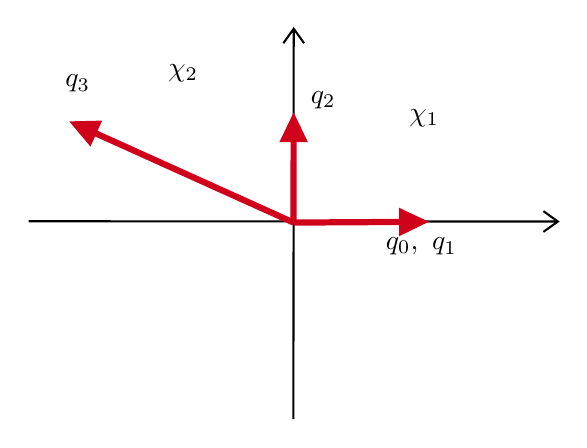
\begin{tikzpicture}[x=0.75pt,y=0.75pt,yscale=-1,xscale=1]
	%uncomment if require: \path (0,252); %set diagram left start at 0, and has height of 252
	
	%Shape: Axis 2D [id:dp521058933232561] 
	\draw [line width=0.75]  (220.97,123.04) -- (475.93,123.18)(348.65,30.28) -- (348.49,218.43) (468.93,118.17) -- (475.93,123.18) -- (468.92,128.17) (343.65,37.28) -- (348.65,30.28) -- (353.65,37.28)  ;
	%Straight Lines [id:da16836362624543133] 
	\draw [color={rgb, 255:red, 208; green, 2; blue, 27 }  ,draw opacity=1 ][line width=2.25]    (348.57,123.68) -- (348.61,75.61) ;
	\draw [shift={(348.62,70.61)}, rotate = 90.05] [fill={rgb, 255:red, 208; green, 2; blue, 27 }  ,fill opacity=1 ][line width=0.08]  [draw opacity=0] (14.29,-6.86) -- (0,0) -- (14.29,6.86) -- cycle    ;
	%Straight Lines [id:da8025190099366124] 
	\draw [color={rgb, 255:red, 208; green, 2; blue, 27 }  ,draw opacity=1 ][line width=2.25]    (348.57,123.68) -- (408.73,123.33) ;
	\draw [shift={(413.73,123.3)}, rotate = 179.67] [fill={rgb, 255:red, 208; green, 2; blue, 27 }  ,fill opacity=1 ][line width=0.08]  [draw opacity=0] (14.29,-6.86) -- (0,0) -- (14.29,6.86) -- cycle    ;
	%Straight Lines [id:da840019010653217] 
	\draw [color={rgb, 255:red, 208; green, 2; blue, 27 }  ,draw opacity=1 ][line width=2.25]    (348.57,123.68) -- (245.07,76.99) ;
	\draw [shift={(240.51,74.93)}, rotate = 24.28] [fill={rgb, 255:red, 208; green, 2; blue, 27 }  ,fill opacity=1 ][line width=0.08]  [draw opacity=0] (14.29,-6.86) -- (0,0) -- (14.29,6.86) -- cycle    ;
	
	% Text Node
	\draw (391.74,129.8) node [anchor=north west][inner sep=0.75pt]  [rotate=-0.04] [align=left] {$\displaystyle q_{0} ,\ q_{1}$};
	% Text Node
	\draw (355.61,59.24) node [anchor=north west][inner sep=0.75pt]  [rotate=-0.04] [align=left] {$\displaystyle q_{2}$};
	% Text Node
	\draw (237.33,51.28) node [anchor=north west][inner sep=0.75pt]  [rotate=-0.04] [align=left] {$\displaystyle q_{3}$};
	% Text Node
	\draw (403.06,67.91) node [anchor=north west][inner sep=0.75pt]  [rotate=-0.04] [align=left] {$\displaystyle \centerdot \chi _{1}$};
	% Text Node
	\draw (286.97,46.31) node [anchor=north west][inner sep=0.75pt]  [rotate=-0.04] [align=left] {$\displaystyle \centerdot \chi _{2}$};
	
\end{tikzpicture}
	
\end{centering}

Note that $\det V=(0,2)^T$
The characters define GIT quotients: 
\begin{itemize}
	\item  $X_{1}= \mathbb{C}^{4}//_{\chi_{1}}T^{2}= \mathbb{P}(\mathcal{O}_{\mathbb{P}^{1}}\oplus \mathcal{O}_{\mathbb{P}^{1}}(2)) = \mathbb{F}_2$
	\item  $X_{2}= \mathbb{C}^{4}//_{\chi_{2}}T^{2}= \mathbb{P}(1,1,2)$
\end{itemize}

Note that $\mathbb{F}_2$ is the minimal resolution of $\mathbb{P}(1,1,2)$, related by a blow up at its singular point.
\end{example}

Wall crossings can give us other standard birational transformations.

\begin{example}{Atiyah Flop}{Atiyah Flop}
Consider the action of $\mathbb{C}^{*}$ on $\mathbb{C}^3$ with weights $(1,1,-1)$. 
There are two quotients: $X_+$ corresponding to the chamber with the weights $(1,1)$, i.e. take the unstable locus to be $x=y= 0$, or $X_-$ corresponding to the chamber with $-1$, i.e. take unstable locus $z = 0$. With these stability conditions we have $$
X_{+}= \mathcal{O}(-1)_{\mathbb{P}^{1}} \qquad X_{-}= \mathbb{C}^2, $$ where the wall crossing from the $X_-$ to $X_+$ give the blow up at a point. 

Now suppose $\mathbb{C}^*$ now acts on $V = \mathbb{C}^4$  with coordinates $x_{1}, x_{2}, y_{1},y_{2}$, and weight matrix $Q = \begin{pmatrix}1&1&-1&-1\end{pmatrix}$. 
Defines two chambers in the secondary fan: $\chi_{+}>0$ and $\chi_{-}<0$, so we get unstable locus $x_{1}= x_{2}= 0$ and $y_{1}= y_{2}=0$. Hence $$
X_{+}\simeq \mathcal{O}(-1)_{\mathbb{P}^{1}}^{\oplus_{2}}\simeq X_-
$$This is an example of the Atiyah flop, related by a blow up and its flopping contraction. 
\end{example}

We say a variety is a minimal model if has nef canonical divisor. In the GIT picture, we say a GIT quotient is minimal if $-\det V$ lies in the closure of the chamber corresponding to the variety. 

\subsubsection{Wall Crossing Formula}

cf.~\cite{Kite_2022,ballard_mori_2013} Let $V$ be a vector space of dimension $n$, and let $T$ be an algebraic torus.

Let $V$ be a vector space of dimension $n$, and let $T$ be an algebraic torus. Denote $\det V = \sum_i q_i$, where $q_i$ is the $i^\mathrm{th}$ column of the weight matrix $Q$. 

\begin{definition}{1-Parameter Subgroup}{1-PS}
    Given a reductive, linear algebraic group $G$, we call a one parameter subgroup of $G$ (the image of) an injective homomorphism $\lambda : \mathbb{G}_{m}\to G$. If $G$ acts on a space $V$, this induces an action of $\mathbb{G}_m$ on $V$ defined by $\lambda$, of which we denote the fixed locus $V^\lambda$. 
\end{definition}

Consider a toric GIT problem defined by the action of a group $T$ on a vector space $V$. Let $C_+$ and $C_-$ be adjacent chambers of the secondary fan in $\mathbb{L}^{\vee}_\mathbb{R}$ separated by a wall $W$. Assume that $\det V$ is on the $C_{+}$ side of the adjoining wall $W$. The wall $W$ corresponds to an orthogonal (primitive) one-parameter subgroup $\lambda_{W}\in \mathbb{L}$.

We can define a value $\mu = (\det V)(\lambda_W)$. Let $\lambda_W$ be such that $\mu \geq 0$, so is pointing to the $C_-$ side of the wall. $\mu$ is a combinatorial value which will (roughly) tell us which chamber admits the `bigger' GIT quotients. 

Let $X_+$ (resp. $X_-$) be the GIT quotient $V // _{\theta_{+}}T$ (resp. $V // _{\theta_{-}}T$ ) corresponding to the chosen generic stability condition $\theta_{+}\in C_+$ (resp. $\theta_-$).  Recall from the previous section that GIT quotients are invariant across stability conditions in the interior of a given chamber. 

We can define a somewhat `smaller' GIT problem associated to a subset $S \subset \{ 1,\dots,n \}$, or more specifically a subset $Q_S$ of the weights corresponding to the set $S$, which in our case are the $s_i$ columns of the weight matrix for $s_{i}\in S$. These weights generate a sublattice $L_{S}^\vee\subset L_\mathbb{R}^\vee$, allowing us to define a GIT problem from the exact sequence $$M_{S}\to \mathbb{Z}^{S}\xrightarrow{Q_{S}}L_{S}^{\vee}$$

This GIT problem gives us a strictly lower dimensional variety $Z$, which is a GIT quotient of the fixed locus $V^{\lambda_{W}}$ by $T/\lambda_W$ (where here $T/ \lambda_W$ is the quotient by the image of $\mathbb{G}_m$ under $\lambda$). Here, our subset $Q_S$  is the collection of weights which are orthogonal to $\lambda_W$, that is, the weights which lie in the space spanned by $W$. We can see that lattice $\mathbb{L}_S^\vee$ is exactly the character lattice for the action of $T/\lambda_W$, since the the weights span the space orthogonal to $\lambda_W$. Moreover, the subspace of $V$ fixed by $\lambda_W$ corresponds to the lattice $\mathbb{Z}^S$ in the exact sequence. We choose a character $\theta_W$ in the interior of the wall $W$, to form the quotient $$Z = V^{\lambda_{W}} / /_{\theta_{W}} \left( T/ \lambda_{W}\right) . $$


\begin{definition}{Wall data}{}
	Given a wall $W$ in the secondary fan, define the Wall Datum as the tuple $(Z, \mu)$, where $\mu = (\det V)(\lambda_W)$ and $Z = V^{\lambda_{W}} / /_{\theta_{W}} \left( T/ \lambda_{W}\right)$ as described above. 
\end{definition}

Hence we get the theorem due to~\cite{halpernleistner2014derived} and~\cite{ballard2014variation}.

\begin{theorem}{Wall Crossing Formula}{wall crossing formula}
Consider GIT quotients $X_{+},X_{-}$  related by a wall crossing across W  with wall datum $(Z, \mu)$ as described above. 

If $\mu > 0$, we have a semi-orthogonal decomposition given by $$\mathcal{D}(X_{+}) = \left< \mathcal{D}(X_{-}),\mathcal{D}(Z) , \dots, \mathcal{D}(Z)  \right>$$ with $\mu$ copies of $\mathcal{D}(Z)$ appearing.

If $\mu = 0$, the wall crossing induces a flop, and we have an equivalence of categories $$\mathcal{D}(X_{+})\simeq \mathcal{D}(X_-).$$
\end{theorem}

This theorem was proved in~\cite{ballard2014variation} in much greater generality than used here, where such a decomposition holds for a smooth quasi-projective variety acted upon by a linear algebraic group, and a wall-crossing between two G-equivariant line bundles. However, to state the theorem in full generality requires more technical machinery than is necessary for the toric case for the purposes of our examples below. 

\begin{example}{}{}
    Recall Beilinson's exceptional collection~\cite{Beilinson1978} which forms a SOD of $\mathcal{D}(\mathbb{P}^n)$. Since $\mathbb{P}^n$ is a toric variety, we can realise it as the GIT quotient with respect to the usual action of $\mathbb{C}^*$ on $V = \mathbb{C}^{n+1}$. So the weights are $\begin{pmatrix}1 & 1 &\dots &1\end{pmatrix}$, with $\det V = n+1$. The wall crossing to $X_{-}=\emptyset$, retrieves the decomposition $\left< pt, \dots,pt \right>$ with $n+1$ copies of the derived category of a point, corresponding to the exceptional collection of line bundles on $\mathbb{P}^n$. 
\end{example}

\begin{example}{}{}
	Recall the wall crossing of example~\ref*{ex:Atiyah Flop}, where the action of $\mathbb{C}^{*}$ on $\mathbb{C}^3$ with weights $(1,1,-1)$ gives $$X_{+}= \mathcal{O}(-1)_{\mathbb{P}^{1}} \qquad X_{-}= \mathbb{C}^2, $$ The wall crossing formula gives us the decomposition $$\mathcal{D}(\mathcal{O}(-1)_{\mathbb{P}^{1}})= \left< \mathbb{C}^{2}, pt \right> $$ which recovers Orlov's blow-up formula from theorem~\ref*{thm:blowupformula}.
\end{example}

\begin{example}{}{}
    Now consider the action of $\mathbb{C}^{*}$ on $\mathbb{C}^3$ with weights $(1,1,-2)$ corresponding to coordinates $x_{1},x_{2},y_1,y_2$ .  Since $\det V = 0$, any wall crossing will give us a flop. Indeed, we have stability conditions, giving quotients $$X_{+}= \mathcal{O}_{\mathbb{P}^{1}}(-2) \qquad X_{-}= [\mathbb{C}^{2}/ \mathbb{Z}_2]  $$where $[\mathbb{C}^2/\mathbb{Z}_2]$ is the orbifold with the action of $\mathbb{Z}_2$. Then we get a derived equivalence $$\mathcal{D}(\mathcal{O}_{\mathbb{P}^{1}}(-2))\simeq \mathcal{D}([\mathbb{C}^{2}/\mathbb{Z}_{2}])$$
\end{example}


\subsubsection{Homological Mori Program}

The above theorem immediately yields a method for calculating a semi-orthogonal decomposition which is `maximally refined', in that none of its components can be factored further through wall-crossings. This follows a similar algorithm to the toric Mori program. Indeed, in such a GIT problem, a sequence of adjacent wall crossings come from sequences of birational operations, specifically directed flips, flops and divisorial contractions. This sequence can be seen by considering a path $\gamma : [0,1] \to \mathbb{L}^\vee$ in the cocharacter lattice, such that $\gamma(0)$ is in the ample cone of the secondary fan,$\gamma$ does not intersect a codimension 2 cone in $\mathbb{L}^\vee$, and $\gamma(1)$ is outside the support of the fan. Such a path $\gamma$ is called a run of the toric Mori program.

Starting with some fixed stability condition $\theta _1$ and its corresponding variety $X_1$, a wall crossing across the wall $W$ (away from $\det V$) gives the decomposition into $X_2$, the variety defined by the wall crossing, and $\mu$ copies of the variety $Z_W$, the variety defined by the wall datum for $W$. We can perform repeated wall crossings to decompose $X_2$ until a minimal model $X_{min}$ is reached. We will then be left with a factor of $X_{min}$ , and factors corresponding to the GIT problems $V^{\lambda_{W}} / / \lambda_{W}$ for each wall $W$ crossed, and can hence repeat the process of decomposition on each of the remaining non-minimal factors.

\begin{example}{Running the toric Mori program \cite{Kite_2022}}{}
	Let $(\mathbb{C}^*)^2$ act on $\mathbb{C}^6$ with weights $$Q = \begin{pmatrix}
		1&1&-1&0&0&0\\ 0&0&1&1&1&-1
	\end{pmatrix}$$
	Which gives secondary fan below
	\tikzset{every picture/.style={line width=0.75pt}} %set default line width to 0.75pt        

\begin{centering}	

	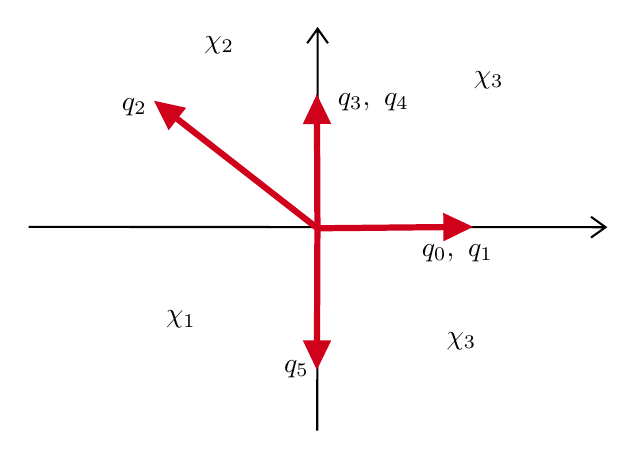
\begin{tikzpicture}[x=0.75pt,y=0.75pt,yscale=-1,xscale=1]
	%uncomment if require: \path (0,252); %set diagram left start at 0, and has height of 252
	
	%Shape: Axis 2D [id:dp521058933232561] 
	\draw [line width=0.75]  (211.98,127.56) -- (489.91,127.71)(351.16,32.07) -- (350.99,225.76) (482.91,122.7) -- (489.91,127.71) -- (482.9,132.7) (346.16,39.07) -- (351.16,32.07) -- (356.16,39.08)  ;
	%Straight Lines [id:da16836362624543133] 
	\draw [color={rgb, 255:red, 208; green, 2; blue, 27 }  ,draw opacity=1 ][line width=2.25]    (351.08,128.22) -- (350.84,68.69) ;
	\draw [shift={(350.82,63.69)}, rotate = 89.77] [fill={rgb, 255:red, 208; green, 2; blue, 27 }  ,fill opacity=1 ][line width=0.08]  [draw opacity=0] (14.29,-6.86) -- (0,0) -- (14.29,6.86) -- cycle    ;
	%Straight Lines [id:da8025190099366124] 
	\draw [color={rgb, 255:red, 208; green, 2; blue, 27 }  ,draw opacity=1 ][line width=2.25]    (351.08,128.22) -- (421.04,127.57) ;
	\draw [shift={(426.04,127.52)}, rotate = 179.47] [fill={rgb, 255:red, 208; green, 2; blue, 27 }  ,fill opacity=1 ][line width=0.08]  [draw opacity=0] (14.29,-6.86) -- (0,0) -- (14.29,6.86) -- cycle    ;
	%Straight Lines [id:da840019010653217] 
	\draw [color={rgb, 255:red, 208; green, 2; blue, 27 }  ,draw opacity=1 ][line width=2.25]    (351.08,128.22) -- (276.27,69.86) ;
	\draw [shift={(272.33,66.78)}, rotate = 37.96] [fill={rgb, 255:red, 208; green, 2; blue, 27 }  ,fill opacity=1 ][line width=0.08]  [draw opacity=0] (14.29,-6.86) -- (0,0) -- (14.29,6.86) -- cycle    ;
	%Straight Lines [id:da3402485134499953] 
	\draw [color={rgb, 255:red, 208; green, 2; blue, 27 }  ,draw opacity=1 ][line width=2.25]    (351.08,127.63) -- (350.84,191.49) ;
	\draw [shift={(350.82,196.49)}, rotate = 270.22] [fill={rgb, 255:red, 208; green, 2; blue, 27 }  ,fill opacity=1 ][line width=0.08]  [draw opacity=0] (14.29,-6.86) -- (0,0) -- (14.29,6.86) -- cycle    ;
	
	% Text Node
	\draw (400.12,134.79) node [anchor=north west][inner sep=0.75pt]  [rotate=-0.04] [align=left] {$\displaystyle q_{0} ,\ q_{1}$};
	% Text Node
	\draw (359.64,62.15) node [anchor=north west][inner sep=0.75pt]  [rotate=-0.04] [align=left] {$\displaystyle q_{3} ,\ q_{4}$};
	% Text Node
	\draw (255.65,64.24) node [anchor=north west][inner sep=0.75pt]  [rotate=-0.04] [align=left] {$\displaystyle q_{2}$};
	% Text Node
	\draw (276.88,166.81) node [anchor=north west][inner sep=0.75pt]  [rotate=-0.04] [align=left] {$\displaystyle \centerdot \chi _{1}$};
	% Text Node
	\draw (295.31,34.42) node [anchor=north west][inner sep=0.75pt]  [rotate=-0.04] [align=left] {$\displaystyle \centerdot \chi _{2}$};
	% Text Node
	\draw (333.78,190.58) node [anchor=north west][inner sep=0.75pt]   [align=left] {$\displaystyle q_{5}$};
	% Text Node
	\draw (425.14,51.51) node [anchor=north west][inner sep=0.75pt]  [rotate=-0.04] [align=left] {$\displaystyle \centerdot \chi _{3}$};
	% Text Node
	\draw (412.05,177.11) node [anchor=north west][inner sep=0.75pt]  [rotate=-0.04] [align=left] {$\displaystyle \centerdot \chi _{3}$};
	\end{tikzpicture}
	
\end{centering}

Since the anticanonical is $\begin{pmatrix}
	1\\2
\end{pmatrix}$, we will start the run of the toric Mori program in the chamber containing $\chi_3$, along a straight-line path intersecting the walls $\left<q_3,q_4\right>_+$ and $\left<q_2\right>_+$. 

The irrelevant ideal is $Irr(\chi_3) = \left< x_3 x_0,x_4 x_0, x_3 x_1 , x_4 x_1 , x_2 x_0 , x_2 x_1 \right>$, so the GIT quotient is $X_{3}= \mathbb{C}^6 \setminus X^{ss} (\chi_3)/ (\mathbb{C}^*)^2 = \mathrm{Tot} (\mathcal{O}(-1)_P)$ for $P = \mathbb{P}(\mathcal{O}^{\oplus 2} \oplus \mathcal{O}(-1))_{\mathbb{P}^1}$. From here, we cross the wall $\left<  q_{3}, q_4\right>_+$. $Irr(\chi_{2})= \left<  x_{2}x_{3}, x_{2}x_{4}, x_{2}x_{1}, x_{2}x_{0}\right>$, so $X_{2}= \mathbb{C}^{2} \setminus X^{ss}(\chi_{2})/ (\mathbb{C}^{*})^{2}= \mathcal{O}(-1)_{\mathbb{P}^3}$.  The wall between them has 1-PS $\begin{pmatrix}1\\0\end{pmatrix}$, so $\mu = 1$. $\mathrm{Tot }(\mathcal{O}(-1)_P)$ is a blow up of $\mathrm{Tot}(\mathcal{O}(-1)_{\mathbb{P}^3})$ along $\mathcal{O}(-1)_{\mathbb{P}^1}$, so the blow up formula gives wall data  $(Z = \mathcal{O}(-1)_{\mathbb{P}^1},1)$, giving the decomposition $$
\mathcal{D}(X_{3})= \left< X_{2}, \mathcal{O}(-1)_{\mathbb{P}^1} \right> 
$$
Now let's cross the wall $\left< q_2 \right>_+$. This has 1-PS $\begin{pmatrix}1\\1\end{pmatrix}$, so $\mu= 3$. 
$Irr (\chi_{1})= \left< x_{2}x_{5} \right>$, so $X_{1}= (\mathbb{C}^{6}\setminus \{ x_{2}= 0 \}\cup \{ x_{5}= 0 \})/ (\mathbb{C}^{*})^{2}= \mathbb{C}^4$. We can see that $\mathcal{O}(-1)_{\mathbb{P}^3}$ is the blow up of $\mathbb{C}^4$ at a point, so  the wall data is $(\mathbb{C}^{2} , 3)$, giving $$
\mathcal{D}(X_{2})= \left< pt, pt, pt , \mathbb{C}^2 \right> 
$$
Recall from Example~\ref{ex:Atiyah Flop}, $\mathcal{O}(-1)_{\mathbb{P}^1}$ is a toric GIT quotient defined by the blow up of $\mathbb{C}^2$ at a point, so we have $$
\mathcal{D}(\mathcal{O}(-2)_{\mathbb{P}^{1}})= \left<  pt, \mathbb{C}^2 \right> 
$$hence we have the decomposition $$
\mathcal{D}(X_{3}) = \left<  pt , \mathbb{C}^{2}, pt , pt, pt, \mathbb{C}^2 \right> .
$$

\end{example}

We are interested in finding examples of nontrivial equivalences of derived categories induced by flops, which in the toric picture can be seen by considering the Calabi-Yau case.From this, it is clear that $\mu = 0$ for all walls $W$ in the secondary fan, so any wall crossing induces a flop on the GIT quotients. Moreover, this gives us a way to see the nontrivial autoequivalences which come from these wall crossings. In particular, we will see that these autoequivalences have a nice interpretation as twists around spherical functors. 

\subsection{Windows and Spherical functors}

First, we want to make some generalizations on the theory of spherical objects. Recall that a spherical object $\mathcal{E} \in \mathcal{D}(X)$ satisfies the property that $$\mathrm{Hom}(\mathcal{E}, \mathcal{E}[i])= \begin{cases}
\mathbb{C} & i=0,\mathrm{dim}X  \\
0 & \text{otherwise}
\end{cases}$$
and the spherical twist of an object $\mathcal{F}$ around $\mathcal{E}$ is an autoequivalence defined as the cone $$T_\mathcal{E} = C(\mathrm{Hom}(\mathcal{E},\mathcal{F})\otimes \mathcal{E}\xrightarrow{ev} \mathcal{F})$$
We define spherical functors analogously.

\begin{definition}{}{}
	A functorial exact triangle is a `triangle' of exact functors $F_{1}, F_{2}, F_{3} : \mathcal{C}\to \mathcal{D}$,    equipped with natural transformations $$
F_{1}(-)\to F_{2}(-)\to F_{3}(-)\to F_{1}(-)[1]
$$ such that for every object $\mathcal{F}\in \mathcal{C}$,   we get the exact triangle in $\mathcal{D}$ given by $$
F_{1}(\mathcal{F})\to F_{2}(\mathcal{F})\to F_{3}(\mathcal{F})\to F_{1}(\mathcal{F})[1]
$$
\end{definition}

Consider an adjoint pair of exact functors $L \dashv R$. Let $\eta : \mathrm{Id}_\mathcal{D}\to R\circ L$ be the unit and $\epsilon : L\circ R \to \mathrm{Id}_\mathcal{C}$ the counit. 

\begin{definition}{}{}
A functor between triangulated categories $F: \mathcal{A}\to \mathcal{B}$ is called spherical if it admits an adjunction $F^{*}\dashv F$ and  functorial exact triangles 
\begin{align*}
F^{*}F \xrightarrow{\epsilon} \mathrm{Id}_\mathcal{A}&\to T \to F^{*}F [1] \\
C\to \mathrm{Id}_\mathcal{B}&\xrightarrow{\eta} F F^{*}\to C[1]
\end{align*} such that $T$ and $C$ are equivalences. Then we call $T$ (resp. $C$) the spherical twist(resp. cotwist) along $F$. 
\end{definition}

Let $X_+$ and $X_-$ be two toric varieties related by a flop induced from a wall crossing in a Calabi-Yau GIT problem. In the formulation of the wall-crossing decomposition, we get a variety $Z$ from the wall $W$ which may appear in as a factor. $Z$ is the toric variety arising from the GIT problem induced by a character on the ray spanned by the wall. In ~\cite{halpernleistner2016autoequivalences}, they show that we have countably infinitely many equivalences $\psi_{i}: \mathcal{D}(X_{-})\xrightarrow{\sim} \mathcal{D}(X_{+})$  such that the autoequivalence $\psi_{i+1}^{-1}\circ \psi_i$ of $\mathcal{D}(X_{-})$ is a spherical twist around a spherical functor $$F : \mathcal{G}\to \mathcal{D}(X_{-})$$ for a category $\mathcal{G}$ (to be defined later).

We examine this twist in more detail for the case of the standard flop (cf.~\cite{donovan_window_2014}) before stating the more general theorem. 

Recall once more the action of $T = \mathbb{C}^*$ on $V = \mathbb{C}^4$  acting on coordinates $x_{1}, x_{2}, y_{1},y_{2}$ with weights $\begin{pmatrix}1&1&-1&-1\end{pmatrix}$ respectively. So $X_+$ and $X_-$ are both isomorphic to $\mathcal{O}(-1)_{\mathbb{P}^1}^{\oplus_{2}}$, related by a flop along the zero section $\mathbb{P}^1_{x_{1},x_{2}}$ or vice versa. Clearly their derived categories are equivalent. Since $X_+$ and $X_-$ are the quotients of $V$ minus an unstable locus ($x_{1}= x_{2}= 0$ or $y_{1}= y_{2}=0$)  by $T = C^{*}$, we can view them as sub-quotient stacks of the Artin quotient stack $\mathfrak{X}=[V/T]$, with derived category $\mathcal{D}(\mathfrak{X})$. We thus have the inclusions $$
i_{\pm}: X_{\pm}\to \mathcal{X}
$$
Note that $\mathcal{D}(\mathfrak{X})$ contains the line bundles $\mathcal{O}(i)$ (corresponding to characters of $\mathbb{C}^*$).  Hence we define subcategories of $\mathcal{D}(\mathfrak{X})$ by $$
 \mathcal{W}_{t}= \left< \mathcal{O}(t), \mathcal{O}(t+1) \right> 
$$ for any $t \in \mathbb{Z}$. We can restrict the pullback of the inclusions to get equivalences $$
i^{*_{\pm}}:\mathcal{W}_{t} \xrightarrow{\sim} \mathcal{D}(X_{\pm})
$$
This equivalence can be verified by considering that $X_\pm$ is a quasi-projective variety, so we can make use of Beilinson's theorem stating that $\mathcal{O}(t), \mathcal{O}(t+1)$ is a strong, full, exceptional collection on $\mathbb{P}^1$, so the direct summands of the bundle $\mathcal{O}(t)\oplus \mathcal{O}(t+1)$ generate  $\mathcal{D}(\mathcal{O}(-1)_{\mathbb{P}^{1}}^{\oplus {2}})$.  Hence we can define the equivalence and then autoequivalence $$
\psi_{t}:= i_{+}\circ i_{-}^{*}: \mathcal{D}(X_{-})\to \mathcal{D}(X_{+}) \qquad \Phi_{t}:= \psi_{t-1}^{-1}\psi_{t}: \mathcal{D}(X_{-})\to \mathcal{D}(X_{-})
$$
We call $\mathcal{W}_t$ a window subcategory, in that $\mathcal{D}(X_{-})$is passing through a smaller intermediate than the whole of $\mathcal{D}(\mathfrak{X})$. Moreover, the autoequivalence can be composed from passing through any two windows, i.e. $$
w_{l,t}:= \psi_{l}^{-1}\psi_t
$$
This is called the `window shift'. 

\begin{remark}{}{}
	The method from this examples can be generalized to the action of $\mathbb{C}^*$ on $\mathbb{C}^k$ so long as the GIT problem is still Calabi-Yau. Assuming the sum of the positive weights is $d$ (so the sum of the negative weights is $-d$), window shift autoequivalences can be constructed with the subcategory $$\mathcal{W}_{t}= \left< \mathcal{O}(t),\dots, \mathcal{O}(t+d-1) \right> $$
\end{remark}


Consider the effect of $\Phi_t$ on our generators $\mathcal{O}(t)$ and $\mathcal{O}(t+1)$. Clearly $\psi_t$ sends both line bundles to themselves on $X_{+}$. Next we apply $\psi_{t-1}^{-1}$, but first both line bundles need to be resolved in such a way that they are written in terms of $\mathcal{O}(t-1)$ and $\mathcal{O}(t)$. We already have this for $\mathcal{O}(t)$. For $\mathcal{O}(t+1)$, the pullback of the Euler sequence on the zero section $\mathbb{P}^1$ gives the Koszul resolution $$
 0\to \mathcal{O}(2)\xrightarrow{\begin{pmatrix}x_2\\-x_{1}\end{pmatrix}}\mathcal{O}(1)^{\oplus 2}\xrightarrow{\begin{pmatrix}x_{1}&x_2\end{pmatrix}} \mathcal{O}
$$so $\mathcal{O}(t+1)$ is quasi-isomorphic to the complex $\left[ \mathcal{O}(t)^{\oplus{2}}\to \mathcal{O}(t-1) \right]$, and we have image of each generator under $\Phi_t$ . 
\begin{align*}
\mathcal{O}(t) &\mapsto \mathcal{O}(t)\\
\mathcal{\mathcal{O}}(t+1)&\mapsto\left[ \mathcal{O}(t)^{\oplus 2}\to \mathcal{O}(t-1) \right][-1] .
\end{align*}

We can see that computing the image of an arbitrary object in $\mathcal{E} \in \mathcal{D}(X_-)$ under $\Phi_t$ requires us to resolve $\mathcal{E}$ in terms of the generators of the first window, then resolve $\psi_{t}(\mathcal{E})$ in terms of generators of the second. This becomes more difficult in the general case.  \cite{donovan_window_2014} shows the existence of an endofunctor on the ambient quotient stack $\mathfrak{T}: \mathcal{D}(\mathfrak{X})\to \mathcal{D}(\mathfrak{X})$ which identifies objects from one window with another, called the Transfer Functor. To see it in action, let's consider the case of $t = 1$.

Since both $X_-$ and $X_+$ have exceptional locus $\mathbb{P}^1$, which can both be contracted to a point giving us the following maps $$
\left\{ pt \right\} \xleftarrow{\pi} \mathbb{P}^{1}\xrightarrow{j} X_{-}
$$
This can be generalised to maps from the substack identified with the quotient of $\mathbb{C}^{2}_{y_{1}, y_{2}} \oplus \{ 0 \}$ by $\mathbb{C}^*$, giving the correspondence $$
\{ pt \}\xleftarrow{\Pi}[\mathbb{C}^{2}/\mathbb{C}^*] \xrightarrow{J} \mathfrak{X}
$$
The transfer functor is then defined as the twist around the functor $\mathfrak{R}:= \Pi_{*}J^{!}: \mathcal{D}(X_{-})\to \mathcal{D}(\{ pt \})$  with left adjoint $\mathfrak{L}:= J_{*}\Pi^{*}$, given by $$
\mathfrak{T}:= \mathrm{Cone}\left(\mathfrak{L}\circ \mathfrak{R} \to \mathrm{Id}_{\mathcal{D}(\mathfrak{X})} \right) 
$$
This functor restricts to an autoequivalence $T: \mathcal{D}(X_{-})\to \mathcal{D}(X_-)$ which is similarly the twist for the adjunction $L\dashv R= \pi_{*}j^{!} : \mathcal{D}(X_{-})\to \mathcal{D}(\left\{ pt \right\})$. That is, $T$ fits into a functorial exact triangle $$
L\circ R \xrightarrow{\epsilon} \mathrm{Id}_{\mathcal{D}(X_{-})} \to T\to L\circ R[1]
$$Where $T$ is the cone on the counit $\epsilon$. 


\begin{theorem}{\cite{donovan_window_2014}}{}
	 $T$ is the same as $\Phi_1$. 
\end{theorem}

\begin{proof}
	
The proof of this statement relies on $\mathfrak{T}$ satisfying three key conditions. 

First, $\mathfrak{T}$ must send $\mathcal{W}_1$ to $\mathcal{W}_{0}$. This follows from that fact that the relative canonical sheaf $\omega_J$ of $J$ is $\mathcal{O}(-2)$ with relative dimension $-2$, so we have 
\begin{align*}
\Pi_{*}J^{!}(\mathcal{O}(1)) &= \Pi_{*}\left(\omega_{J}\otimes  J^{*} \mathcal{O}(1)[-2] \right) \\
&= \Pi_{*}\left( \mathcal{O}(-2)\otimes  J^{*}\mathcal{O}(1)[-2] \right) \\
&= \Pi_{*}\mathcal{O}(-1)[-2] \\
&=0  
\end{align*}

Hence $\mathfrak{L} \circ \mathfrak{R} (\mathcal{O}(1))=0$, and the cone on $\epsilon$ is the identity, so $\mathfrak{T}(\mathcal{O}(1)) = \mathcal{O}(1)\in \mathcal{W_0}$.

For $\mathcal{O}(2)$, 
\begin{align*}
\Pi_{*}J^{!}(\mathcal{O}(2)) &= \Pi_{*}\left(\omega_{J}\otimes  J^{*} \mathcal{O}(2)[-2] \right) \\
&= \Pi_{*}\left( \mathcal{O}(-2)\otimes  J^{*}\mathcal{O}(2)[-2] \right) \\
&= \Pi_{*}\mathcal{O}[-2] \\
&= \mathcal{O}_{pt}[-2]
\end{align*}

Pulling back from the point and pushing forward onto $\mathfrak{X}$, we get the sheaf $\mathcal{O}_{\mathbb{C}^{2}}[-2]$. We want to take the cone on the natural transformation $$
\mathcal{O}_{\mathbb{C}^2}[-2]\xrightarrow{\epsilon} \mathcal{O}(2)
$$ The exact sequence $$
0 \to \mathcal{O}(2)\to \mathcal{O}(1) ^{\oplus 2} \to \mathcal{O} \to \mathcal{O}_{\mathbb{C}^{2}}\to 0
$$ shows us that $\mathcal{O}_{\mathbb{C}^2}[-2]$ is quasi-isomorphic to $\left[ \mathcal{O}(2)\to \mathcal{O}(1)^{\oplus{2}}\to \mathcal{O} \right][-2]$, to taking the cone over $\epsilon$ gives us $\left[ \mathcal{O}^{\oplus{2}}\to \mathcal{O} \right][-1] \in \mathcal{W}_0.$

Hence we have 
\begin{align*}
\mathcal{O}(1) &\mapsto \mathcal{O}(1) \\
\mathcal{O}(2) &\mapsto \left[ \mathcal{O}(1)^{\oplus_{2}}\to \mathcal{O} \right][-2] 
\end{align*}

Which gives us the diagram

\[\begin{tikzcd}
	{\mathcal{W}_1} && {\mathcal{W}_0} \\
	& {\mathcal{D}(X_+ )} \\
	{\mathcal{D}(X_- )} && {\mathcal{D}(X_- )}
	\arrow["{\mathfrak T}", from=1-1, to=1-3]
	\arrow["{i_+^*}"', from=1-1, to=2-2]
	\arrow["{i_- ^*}"', from=1-1, to=3-1]
	\arrow["{i_+^*}", from=1-3, to=2-2]
	\arrow["{i_- ^*}", from=1-3, to=3-3]
	\arrow["{\psi_1}", from=3-1, to=2-2]
	\arrow["T", from=3-1, to=3-3]
	\arrow["{\psi_0}"', from=3-3, to=2-2]
\end{tikzcd}\]

Secondly, the upper triangle commutes because $\mathfrak{T}$ must act trivially outside $\mathbb{C}^{2}_{y_{1},y_{2}}\oplus \{ 0 \}$, i.e. $$
i^{*}_{+}\mathfrak{T} = i^{*}_{+}
$$This is a given from the definition, since objects on $X_+$ are in the kernel of the composition $\mathfrak{L}\circ\mathfrak{R}$, so $\mathfrak{T}$ acts as the identity. 

Thirdly,  $\mathfrak{T}$ must restrict to $T$, i.e. the rectangle commutes. This is due to generators $\mathcal{O}$ and $\mathcal{O}(-1)$ not having higher cohomology, so the derived pushforwards $\pi_{*}$ and $\Pi_{*}$ at least give the same thing on $\mathcal{W}_1$ , so $i_{-}^{*}\circ \mathfrak{T} = T\circ i_{-}^{*}$. 

From these, we can conclude that the lower triangle commutes, so $T = \Phi_1$. 
\end{proof}

To relate this back to the usual reference of spherical twist we can look at the functorial exact triangle object-wise, to see that for each object $\mathcal{E}\in \mathcal{D}(X_-)$, $T_F$ is the cone $$
T_{F}(E) = \mathrm{Cone}\left( \mathrm{Hom}(\mathcal{O}_{\mathbb{P}^{1}},\mathcal{E}) \otimes  \mathcal{O}_{\mathbb{P}^{1}} \to \mathcal{E}\right) 
$$ 

\begin{remark}{}{}
	This is just one example of a much more general statement about window shifts, and flops in general.~\cite{donovan_window_2014} prove the theorem for Grassmannian flops, which includes the case of the standard flop we just saw. Indeed, for  vector spaces $V$ and $S$ of dimension $d$ and $r \leq d$ respectively, the associated quotient stack for the GIT problem is $$
	\left[ \mathrm{Hom} (S,V) \oplus \mathrm{Hom}(V,S)/\mathrm{GL}(S) \right] 
	$$where the standard flop is the case when $d = 2$, $r=1$.
	\end{remark}

Indeed, the presentation of flop autoequivalences as spherical twists is not limited to GIT quotoients, as proved for a certain simplicity of wall crossings in~\cite{halpernleistner2016autoequivalences}. Barbocovi~\cite{barbacovi_spherical_2021} proves this fact for any flop which induces a derived equivalence, as summarised below.

Let $X_{-}\xleftarrow{p} \hat{X} \xrightarrow{q} X+$ be a flop. Moreover, assume that $p_{*}\mathcal{O}_{\hat{X}}= O_{X_-}$, $q_{*}\mathcal{O}_{\hat{X}}= O_{X_+}$,  and that there are derived equivalences$$
q_{*}p^{*}: \mathcal{D}(X_{-})\to \mathcal{D}(X_{+}), \qquad p_{*}q^{*}: \mathcal{D}(X_{+})\to \mathcal{D}(X_{-})
$$

Note that $p^*$ (resp. $q^{*}$) are left adjoints to $p_*$ (resp. $q_{*}$ ), and the properness and finite Tor dimension gives a right adjoint $p^{\times}: \mathcal{D}(X_{-})\to \mathcal{D}(\hat{X})$ and $q^{\times}: \mathcal{D}(X_{+})\to \mathcal{D}(\hat{X})$. Moreover, these left and right adjoints $p_{*}, p^{*} ,p^{\times}, q_{*}, q^{*},q^{\times}$ are all fully faithful, preserving boundedness and coherence.  

Define $\mathcal{K} = \mathrm{ker}(p_{*}) \cap \mathrm{ker}(q_{*})$ , and $\mathcal{ K}^{b}= \mathcal{K} \cap \mathcal{D}(\hat{X}) \subset \mathcal{D}(\hat{X})$. $\mathcal{K}^b$  is a thick full triangulated subcategory of $\mathcal{D}(\hat{X})$, hence we can take the quotient $Q: \mathcal{D}(\hat{X})\to \mathcal{D}(\hat{X})/\mathcal{K}^b$ , which gives us  induced maps
$$\bar{p}_{*} = \mathcal{D}(\bar{ X})/ \mathcal{K}^{b}\to \mathcal{D}(X_{-})$$

\begin{theorem}{Barbacovi}{}
There is a  four-periodic SOD of $\mathcal{D}(\hat{X})/\mathcal{K}^b$ given by $$
\left< \mathrm{ker}\,\bar{p}_{*},\mathcal{D}(X_{-}) \right> =  \left< \mathcal{D}(X_{+}), \mathrm{ker}\,\bar{q}_{*} \right> = \left< \mathrm{ker}\,\bar{q}_{*} , \mathcal{D}(X_{+})\right> = \left< \mathcal{D}(X_{-}), \mathrm{ker}\,\bar{p}_{*} \right>  
$$ which induces spherical functors $\Psi_{+}: \mathrm{ker} \bar{p}_{*}\xrightarrow{\bar{q}_{*}}\mathcal{D}(X_+)$ and $\Psi_{+}: \mathrm{ker} \bar{q}_{*}\xrightarrow{\bar{p}_{*}}\mathcal{D}(X_-)$ such that the `flop-flop' autoequivalences $FF _{+}:= q_{*}p^{*}p_{*}q^{*}$ and $F F_{-}: = p_{*}q^{*}q_{*}p^*$ are the spherical twists around each functor respectively.
\end{theorem}


\newpage

\section{The cubic fourfold}
In this section, we will review the deep link between K3 surfaces and cubic fourfolds. 

 A theorem of Hasset describes the so called \emph{special cubic fourfolds}, which are cubic fourfolds containing a surface $T$ which is not a complete intersection. They form a countable union of divisors $\calC_d$ in the moduli space $\P H^0(\O(3))/\P GL(6)$ of cubic fourfolds which are expected to be the rational cubic fourfolds (the intuition is that for a cubic fourfold to be rational, one has to blow up a surface at some point) and have associated K3 surfaces: the primitive cohomology of a K3 surface embeds as the complement $\langle h^2, T\rangle^\perp$. 

Alternatively, Kuznetsov has considered the derived category of a cubic fourfold and found a component $\calA_X$. He showed that Pfaffian cubics and nodal cubics have $\calA_X$ derived equivalent to K3 surfaces and conjectured \cite{KuznetsovDerivedCubic} that $X$ is rational if and only if $\calA_X \simeq \calD(S)$ for some K3 surface $S$.

The two viewpoints, the Hodge theoretic of Hassett and derived categorical of Kuznetsov, were shown to be equivalent by \cite{addington_hodge_2014}: in other words, ...

In this section, we will briefly describe the Hodge theory and Torelli theorems for K3 surfaces and cubic fourfolds. After that, we will show that the Kuznetsov component is a Calabi-Yau 2 category and show that the cubic fourfolds containing a plane $\calC_8$ are derived equivalent to a twisted K3 surface, which is an honest K3 surface when $X\in \calC_8 \cap \calC_d$ for some other $d$ on Hasset's list. Finally, we quickly sketch Addington-Thomas' paper.



\subsection{A quick review of K3 surfaces}
\begin{definition}{K3 surface}{K3 surface}
A K3 surface is a compact complex surface with $\omega_{S}$ trivial and $H^1(S,\mathcal{O}_{S})=0$.
\end{definition}

Firstly, spaces derived equivalent to K3 surfaces are also K3 surfaces: their dimensions have to be the same because the Serre functors are isomorphic and hence the orders of the canonical bundles are the same. Similarly, by passage to cohomology, we know that $$\bigoplus_{p-q=i}H^{p,q}(S)\simeq \bigoplus_{p-q=i}H^{p,q}(S')$$
Hence, since $h^{0,1}=h^{1,2}$ by Hodge symmetry and Serre duality, we see that both are zero.

Computations using Riemann-Roch show that $$2=\chi(S,\O_S)=\frac{c_1^2+c_2}{12}\implies c_2(S)=e(S)=24$$
Then Poincare duality shows $b_2=22$. 

The Hodge decomposition tells us that $$H^2(S,\mathbb{C})=H^{2,0}\oplus H^{1,1}\oplus H^{0,2}$$But both $h^{2,0}=h^{0,2}=1$ and hence $h^{1,1}=20$.  The Hodge diamond is thus: \[\begin{tikzcd}[row sep=tiny, column sep=tiny]
    &   & 1  &   &   \\
    & 0 &    & 0 &   \\
  1 &   & 20 &   & 1 \\
    & 0 &    & 0 &   \\
    &   & 1  &   &  
  \end{tikzcd}\]

Moreover, the intersection lattice is $H^2(X,\mathbb{X})=\Lambda=(-E_8)^{\oplus 2}\oplus U^{\oplus 3}$ and $H^2(S,\mathbb{Z})=(1,20,1)$ has signature $(3,19)$.

The Hodge structure on a K3 surface is then essentially determined by $H^{2,0}(S)\subset H^2(S;\mathbb{C})=\Lambda\otimes \mathbb{C}$. Thus, we can consider the period map $$P: \mathcal{M} \rightarrow \P \Lambda \otimes \mathbb{C}$$that sends a K3 surface $S$ to the line $H^{2,0}(S)$.  In fact, a nonzero vector in $H^{2,0}$ has $u^2=0, u \overline{u}>0$, which is the defining equation for the period domain. The local Torelli theorem shows that this is surjective and a local homeomorphism. It is not a global isomorphism: one has to mod out by the automorphisms of the lattice $\Lambda$. In fact, it is known that K3 surfaces are determined by the period map, i.e. by their Hodge structure:

\begin{theorem}{Global Torelli}{Global Torelli}
Two K3 surfaces are isomorphic if and only if there is a Hodge isometry $H^2(X,\mathbb{C})\simeq H^2(Y,\mathbb{C})$.
\end{theorem}

%A Hodge isometry respects the intersection pairing and the Hodge decomposition. 

%Because the canonical bundle of $\mathbb{P}^1$ is $\mathcal{O}(-2)$ and is also isomorphic to the normal bundle by adjunction, we see that $$C\cdot C=\int _{C}c_{1}(\mathcal{O}(-2)) =-2$$
%Such curves define a reflection on the cohomology: $$\begin{gathered}
 
%s_{\delta}:H^2(X,\mathbb{Z})\xrightarrow{}H^2(X,\mathbb{Z})\\
%\alpha\mapsto \alpha + \langle \alpha ,\delta \rangle \delta
%\end{gathered}$$
%Is this induced by a spherical twist? Yes, I think the one given by $\mathcal{O}_{C}$. Let's see why this is true:

%Firstly, $\mathcal{O}_{C}$ is spherical because $$\mathrm{Ext^1}(\mathcal{O}_{C},\mathcal{O}_{C})=H^0(\mathcal{Ext}^1)=H^0(\mathcal{N}_{C/X})=H^0(\mathcal{O}(-2))=0$$The other Ext groups are one-dimensional, by Serre duality. 


%Now, the Todd class of a K3 surface $X$ is given as $(1,0,2)$ so its square root is $(1,0,1)$. Hence, for a vector bundle, we see that $$v(\mathcal{E})=(\mathrm{rk}\,\mathcal{E}, c_{1}\mathcal{E}, \mathrm{rk}(\mathcal{E})+c_{1}(\mathcal{E})^2/2-c_{2}(\mathcal{E}))$$
%So for a rational sphere given by the zero locus of a line bundle $\mathcal{L}$, we see by the resolution $$\mathcal{L}^\lor\xrightarrow{}\mathcal{O}_{X}\xrightarrow{}\mathcal{O}_{C}$$ that $\mathrm{ch}(\mathcal{O}_{C})=\mathrm{ch}(\mathcal{L}^\lor)-\mathrm{ch(\mathcal{O}_{X})}=-c_{1}(\mathcal{L})$. Moreover, $v(\mathcal{L}^\lor)=(1,-\delta,0), v(\mathcal{O}_{X})=(1,0,0)$ and hence $$v(\mathcal{O}_{C})=(0,\delta,0)$$ and this recovers the reflection on $H^2(X,\mathbb{Z})$. 

%Wait it's apparently $\mathcal{O}_{C}(-1)$?

%Next: derived equivalence of K3 surfaces iff Hodge isometry of the Mukai Hodge structure.

%Also: moduli of sheaves

\subsection{Hodge theory of cubic fourfolds}

Let us first think about the Hodge diamond of $X$. Embed $\mathbb{P}^5$ via the Veronese embedding in $\mathbb{P}V_{3,5+1}$, the space of degree 3 polynomials in 6 variables. Then, a hyperplane section of the image of $\mathbb{P}^5$ consists of a linear relation between the basis of monomials of this vector space, and hence is precisely a cubic fourfold $X$. The Lefschetz hyperplane theorem states that then $$H^\bullet(\mathbb{P}^5)\xrightarrow{}H^\bullet (X) \text{ iso for }\bullet<4$$
We thus see, by Poincare duality, that $b_{1}=b_{3}=b_{5}=b_{7}=0$. Similarly, $b_{2}=b_{6}=1$ and must be given by $h^{1,1}$ by Hodge theory. We have that $H^2(X;\mathbb{Z})=\mathbb{Z}$ and the LES from the exponential sequence tells us that $$H^1(X,\mathcal{O}_{X})\xrightarrow{}H^1(X,\mathcal{O}_{X}^*)\xrightarrow{}H^2(X,\mathbb{Z})\xrightarrow{}H^2(X,\mathcal{O}_{X})$$
But the first term is 0, since it is a summand of $H^1(X;\mathbb{C})=0$. The second term is $\mathrm{Pic}(X)$ and the map is $c_1$ which lands in $H^{1,1}$. Since $c_1(K_X)=-3$ it is nonzero, so since $\mathbb{C}=H^2(X;\mathbb{C})=H^{2,0}\oplus H^{1,1}\oplus H^{0,2}$ the only option is for $h^{2,0}=h^{0,2}=0$ and $\mathrm{Pic}(X)=\mathbb{Z}$ generated by a hyperplane. 

Now, the interesting bit is the fourth row, the middle dimensional cohomology. By using the normal bundle sequence, we have that $$c(T_{X})(1+3x)=(1+x)^6=\iota^* c(T_{\mathbb{P}^5})$$We compute $c_1=3x, c_2=6x^2, c_3=2x^3, c_4=9x^4$. Then by Gauss-Bonnet, $$b_{4}+4=\chi(X)=\langle 9x^4, [X] \rangle= 27 $$since $pd(X)=3\omega$. We conclude that $b_4=23$. 

We also have that $H^0(X, \Omega^4)=H^0(X, \mathcal{O}_{X}(-3))=0$ so $h^{4,0}=h^{0,4}=0$. The only bit left is to determine $h^{1,3}=h^{3,1}$. 

Now we can use Hirzebruch-Riemann-Roch for the cotangent bundle of $X$, by computing $$\chi(\Omega_{X})=-h^{1,1}-h^{1,3}=\int _{X}\mathrm{ch(\Omega_{X})}\mathrm{td}(T_{X})=3\int _{\mathbb{P}^5} \omega \,\mathrm{ch}(\Omega_{\mathbb{P}^5}-\mathcal{O}(-3)) \mathrm{td}(T_{\mathbb{P}^5}-\mathcal{O}(3))  $$
Because I am lazy, I used the Macaulay 2 code: 

\begin{lstlisting}[language=Python]
loadPackage "Schubert2"
P5  = flagBundle({1,5}, VariableNames=>{s,q})
T = tangentBundle(P5)
coT = cotangentBundle(P5)
O1 = dual(P5.Bundles#0)
w = chern(1,O1)
NX = O1^**3
coNX = dual(NX)
TX = T - NX
coTX = coT - coNX
Q = 3 *  w*ch(coTX)*todd(TX)
print  integral  Q
\end{lstlisting}
This gives the answer -2, which implies $h^{1,3}=1$.

Can try to compute $h^{2,2}$ similarly: again by Hirzebruch-Riemann-Roch
$$h^{2,2}=\chi(\Omega_{X}^2)=\int_{X} \mathrm{ch}(\Omega^2_{X})\mathrm{td}(TX)  $$
The Macaulay code is: 

\begin{lstlisting}[language=Python] 
coT2X = exteriorPower_2 coTX
A = 3*w*ch(coT2X)* todd(TX)
print integral A
\end{lstlisting}
%can add caption by declaring caption = ...
This gives the correct answer $21$! All in all, the Hodge diamond looks like: 

\begin{center}
\begin{tikzcd}[row sep=tiny, column sep=tiny]
    &   &   &   & 1  &   &   &   &   \\
    &   &   & 0 &    & 0 &   &   &   \\
    &   & 0 &   & 1  &   & 0 &   &   \\
    & 0 &   & 0 &    & 0 &   & 0 &   \\
  0 &   & 1 &   & 21 &   & 1 &   & 0 \\
    & 0 &   & 0 &    & 0 &   & 0 &   \\
    &   & 0 &   & 1  &   & 0 &   &   \\
    &   &   & 0 &    & 0 &   &   &   \\
    &   &   &   & 1  &   &   &   &  
  \end{tikzcd}
\end{center}

The primitive cohomology of the cubic fourfold looks like $(0,1,20,1,0)$ and has signature $(20,2)$ which looks similar to the K3 $H^2(S,\mathbb{Z})$, but that one has signature $(3,19)$. 

We can see that $H^{3,1}\simeq \mathbb{C}$ and similarly to the K3 case we have a period map which to each cubic fourfolds associates a line in the local period domain, which is one of the connected components of the quadric hypersurface $Q\subset \P \Lambda$ defined by $u^2=0$ together with the condition that $-(u, \overline{v})$ is a positive hermitian form. We factor out by automorphisms $\Gamma^+$ of $H^4(X,\mathbb{Z})$ which preserve $(-,-)$ and the hyperplane squared $h^2$, and moreover stabilize $\tilde{\calD}$. The resulting map is $$\mathcal{M}_{\text{cubic fourfolds}}\rightarrow \calD : = \tilde{\calD}/\Gamma^+$$

Voisin \cite{voisin_theoreme_2008} proved the following theorem, by considering the cubic fourfolds containing a plane:

\begin{theorem}{Global Torelli for cubic fourfolds}{Global Torelli for cubic fourfolds}
    The period map for cubic fourfolds is injective.
\end{theorem}

We finish off the Hodge theoretic section by a review of the results of Hassett's paper \cite{hassett_special_2000}. 

The essential idea is as follows: a generic cubic fourfold $X$ has $H^{2,2}_{prim}(X;\mathbb{Z})=0$, but there is a class of \emph{special cubic fourfolds} which contain some integral class $T$. This allows us to pass to a codimension $1$ subspace of $H^{2,2}(X)$ which has a chance of being Hodge isometric to the primitive cohomology of a K3 surface (recall that the issue was that a priori they have different signatures). Explicitly, we have $\langle h^2, T\rangle ^\perp \subset H^{2,2}(X)$ and $H^2_{prim}(S)$ both of signature $(2,19)$. Hassett determines exactly when they could be Hodge isometric:

\begin{theorem}{Hassett}{Hassett}
    There is a Noether-Lefschetz divisor $\calC_d$ in the moduli space of cubic fourfolds, where $d=disc\langle h^2, T\rangle$ for $T\subset X$ a surface not homologous to a complete intersection. This is nonempty precisely when $d>6$ and $d\equiv 0,2 \mod 6$. Moreover, these special cubic fourfolds have an associated K3 surface in the sense above precisely when $d$ is not divisible by $4,9$ or any odd prime $p\equiv -1 \mod 3$
\end{theorem}

The slightly awkward condition will be rephrased later, when we review Addington-Thomas.

\subsection{Derived view of the cubic fourfold}

We now shift gears and look at cubic fourfolds through a derived lens.

Take a cubic fourfold $X$ in $\mathbb{P}^5$. This has canonical bundle $K_{X}=-3H$ so is a Fano of index 3. By using Kodaira vanishing, one can show that $$\mathcal{O}_{X}(-2H), \mathcal{O}_{X}(-H), \mathcal{O}_{X}$$form an exceptional collection. The orthogonal complement is given by $$\mathcal{A}_{X}=\{\mathcal{F}\in \mathbf{D}^b(X)|\,\mathrm{Ext}^\bullet(\mathcal{O}_{X}(-iH), \mathcal{F})=0\}$$This component, named after Kuznetsov, is very interesting, as it looks like the derived category of a K3 surface.

We see that, by \ref{th:HKR}, the Hochschild homology is $HH_\bullet(X)=\mathbb{C}[-2]\oplus \mathbb{C}^{25}\oplus \mathbb{C}[2]$. On the other hand, Hochschild homology is additive with respect to semiorthogonal decomposition, and the three exceptional objects contribute to three copies of $\mathbb{C}$ in degree zero, so we see that $HH_\bullet(\mathcal{A}_X)=\mathbb{C}[-2]\oplus \mathbb{C}^{22}\oplus \mathbb{C}[2]$, which is exactly the Hochschild homology of a K3 surface.

These properties of the category $\mathcal{A}_X$ make it possible that there is an honest, geometric K3 surface associated to $X$. All known cases of cubic fourfolds with associated K3 surfaces are birational to $\mathbb{P}^4$, which led Kuznetsov to conjecture:

\begin{conjecture}{}{Kuznetsov's conjecture}
A cubic fourfold is rational if and only if it there is a K3 surface $S$ such that $\mathcal{D}(S)\simeq \mathcal{A}_X$.
\end{conjecture}

In the subsequent section, we will explain why the Kuznetsov component is a CY2 category and later on focus on the fundamental example of cubics containing a plane.

\subsubsection{The Kuznetsov component is CY2}

We now embark on the proof that the Kuznetsov component is a Calab-Yau 2 category. What this means is that it has a Serre functor which is just given by shifting by $2$, as would be the case if it were the derived category of an honest K3 surface.

%\begin{proposition}{Kuznetsov component is CY2}{Kuznetsov component is CY2}
 %   The category $\mathcal{A}_{X}$ is a CY2 category with Hochschild homology the same as that of a K3 surface. Therefore, it is indecomposable and the semiorthogonal decomposition is maximal.
%  \end{proposition}
    

Let us consider a general degree $d$ hypersurface $X \subset \mathbb{P}^{n+1}$. By adjunction, its canonical bundle is given by $\O(d-n-2)$ and hence its Serre functor is $\otimes \,\O(d-n-2)[n] $. Moreover, the line bundles $\O,\dots,\O(n+1-d)$ are all exceptional and have an orthogonal complement which gives $$\calD(X)=\langle \calA_X,\O,\dots,\O(n+1-d) \rangle $$

\paragraph*{The kernel of the Serre functor}

The left mutation with respect to the admissible subcategory spanned by the line bundles is $$\mL_{\langle \O, \dots, \O(n+1-d) \rangle}\simeq \mL_\O \circ \dots \circ \mL_{\O(n+1-d)}$$

Now we notice the following: the mutation $\mL_{\O(i)}$ fits into an exact triangle $$\Hom(\O(i), F)\otimes \O(i) \xrightarrow{ev} F \rightarrow \mL_{\O(i)} F$$
which follows from \ref{ex:Relative exceptional SOD} applied to $Y=pt$ since $\O(i)$ are exceptional.


On the other hand, we can think of the middle as $\Phi_{\O_\Delta}F$ and the left object as $\Phi_{\O(-i)\boxtimes \O(i)}F$. More precisely, by using the projection and base change formulas:
\begin{gather*}
    \Phi_{\O(-i)\boxtimes \O(i)}F=p_* (p^*\O(i)\otimes q^* \O(-i)q^*F)\simeq p_* q^* F(-i)\otimes \O(i)\simeq\\
    \simeq \O_X \otimes \RG (F(-i))\otimes \O(i)\simeq \RG \RlHom(\O(i),F) \otimes O(i)=\RHom(\O(i),F) \otimes \O(i)
\end{gather*}

Hence, we can conclude that $\mL_{\O(i)}$ is given by a Fourier-Mukai transform with kernel $$[\O(-i)\boxtimes \O(i)\rightarrow \O_\Delta]$$

Now, define $$\mathbf{O}:=\mL_\O \circ (-\otimes \O(1))$$
We see that by \ref{cor:Autoequivalences and mutations}, $$\mathbf{O}^{n+2-d}\simeq \mL_\O \circ \mL_{\O(1)}\circ ... \circ \mL_{\O(n+1-d)}\circ (-\otimes \O(n+2-d))=\mL_{\langle \O, \dots, \O(n+1-d) \rangle} \circ (-\otimes \omega ^{-1})$$

But by \ref{lemma:Serre functors of admissible subcategories}, we know that the inverse of the Serre functor of $\calA_X$ is given by $$\calS_{\calA_X}^{-1} =  \mL_{\langle \O, \dots, \O(n+1-d) \rangle} \circ \calS_X ^{-1}=\mL_{\langle \O, \dots, \O(n+1-d) \rangle} \circ (-\otimes \omega^{-1})[-n]$$

We can thus conclude that $$\calS_{\calA_X}^{-1} = \mathbf{O}^{n+2-d}\circ [-n]$$

If we put $T:=\mathbf{O}|_{\calA_X}$, then we can reinterpret this as $$\calS_{\calA_X}=T^{d-n-2}\circ [n]$$

Recall that $\mL_\O$ had kernel given by $[\O \boxtimes \O \rightarrow \O_\Delta]$. We can compose this with the kernel for $-\otimes \O(1)$ which is $\O_\Delta(1)$ to see that the kernel for $T$ is given by $K_1=[\O(1)\boxtimes \O \rightarrow \O_\Delta(1)]$, i.e. we have an exact triangle $K_1 \rightarrow  \O(1)\boxtimes \O \rightarrow \O_\Delta(1)$. 

Our ultimate aim is to show that a suitable power of the Serre functor is just a shift functor, so we need to understand the kernel for $T^i, i=1,2,\dots, $. For this purpose, we need to convolute $K_1$ with itself multiple times. 

\begin{proposition}{Kernel of Serre functor of Kuznetsov component}{Kernel of Serre functor of Kuznetsov component}   
The kernel $K_1^i$ fits into a sequence $$K_1^i\rightarrow \O(1)\boxtimes \Omega^{i-1}(i-1)\rightarrow \dots \rightarrow \O(i-1)\boxtimes \Omega(1)\rightarrow \O(i)\boxtimes \O \rightarrow \O_\Delta(i)$$
\end{proposition}
\begin{proof}
    We show this by induction.
    
    Firstly, composing with a Fourier-Mukai transform preserves exact triangles, so the same holds for the kernels. We can compose the triangle for $K_1$ with $\O(1)\boxtimes \O, \O_\Delta(1)$ on the left and $K_1$ on the right respectively to get three exact triangles \begin{gather*}
        (\O(1)\boxtimes \O) \circ K_1 \rightarrow (\O(1)\boxtimes \O)  \circ (\O(1)\boxtimes \O) \rightarrow (\O(1)\boxtimes \O) \circ \O_\Delta(1)\\
        \O_\Delta(1)\circ K_1 \rightarrow \O_\Delta(1) \circ (\O(1)\boxtimes \O)  \rightarrow \O_\Delta(1) \circ \O_\Delta(1)\\
        K_1 \circ K_1  \rightarrow (\O(1)\boxtimes \O)\circ K_1 \rightarrow \O_\Delta(1)\circ K_1
    \end{gather*}
    
    We can compute some of these: for example, the middle convolution on the first row is given by $$(\O(1)\boxtimes \O)  \circ (\O(1)\boxtimes \O) ={\pi_{13}}_*\big(\O(1)\boxtimes \O \boxtimes \O \otimes \O \boxtimes \O(1) \boxtimes O\big)=\big(\O(1)\boxtimes \O\big) \otimes H^\bullet(\O(1))$$
    as pushing down is the same as cohomology on the fibers. This is the only computation that involves any cohomology: the others are given by tensoring with the diagonal, which turns the first two triangles into: \begin{gather*}
        (\O(1)\boxtimes \O) \circ K_1 \rightarrow \big(\O(1)\boxtimes \O\big) \otimes H^\bullet(\O(1)) \rightarrow \O(1)\boxtimes \O(1)\\
        \O_\Delta(1)\circ K_1 \rightarrow \O(2)\boxtimes \O \rightarrow \O_\Delta(2)
    \end{gather*}
    
    Now recall the Euler sequence on $\mathbb{P}^{n+1}$, which says that there is an exact triangle $$\Omega(1)\rightarrow \O^{n+2}\rightarrow \O(1)$$
    Since the cohomology of $O(1)$ is $n+2$-dimensional, we can read off from the first exact triangle that $ (\O(1)\boxtimes \O) \circ K_1\simeq \O(1) \boxtimes \Omega(1)$. We can now plug this into the second object in the last triangle, as well as replace the last object in the third triangle by the second triangle to get: $$K_1 \circ K_1 \rightarrow \O(1)\boxtimes \Omega(1)\rightarrow \O(2)\boxtimes \O \rightarrow \O_\Delta(2)$$
    
    Now, assume the statement holds for $i$ (we have just shown it holds for $i=2$). Then we can apply $-\circ K_1$. We notice by the same argument that $\O_\Delta(i)\circ K_1= [\O(i+1)\boxtimes \O \rightarrow \O_\Delta(i+1)]$ and also using cohomology on the fibers and the Euler sequence that $\big( \O(i)\boxtimes O\big)\circ K_1=\O(i)\boxtimes \Omega^1(1)$. What we need to understand is the other parts $\big(\O(i-k)\boxtimes \Omega^{k}(k)\big) \circ K_1$. This can be done by applying $\big(\O(i-k)\boxtimes \Omega^k(k)\big)\circ -$ to the triangle defining $K_1$. What we get is the following: $$\big(\O(i-k)\boxtimes \Omega^k(k)\big)\circ K_1 \rightarrow \O(i-k)\boxtimes \O \otimes H^\bullet(\Omega^k(k+1))\rightarrow \O(i-k)\boxtimes \Omega^k(k+1)$$
    
    Now we need to use a variant of the Euler sequence, \cite[Corollary 17.1.3]{arapura_algebraic_2012}: $$\Omega^{k+1}(k+1)\rightarrow \O^{\binom{n+2}{k+1}}\rightarrow \Omega^k(k+1)$$
    
    This, together with a computation of the cohomology of $\Omega^k(k+1)$ having dimension $\binom{n+2}{k+1}$ (it has only $H^0$ using Bott vanishing etc.), tells us that $\big(\O(i-k)\boxtimes \Omega^{k}(k)\big) \circ K_1=\O(i-k)\boxtimes \Omega^{k+1}(k+1)$. This completes the induction, which is illustrated in the picture below, where the squiggly arrows denote convolution with $K_1$:
        \[\begin{tikzcd}
            {K_1^i} & {\O(1)\boxtimes \Omega^{i-1}(i-1)} & \dots & {\O(i)\boxtimes \O} & {\O_\Delta(i)} \\
            {K_1^{i+1}} & {\O(1)\boxtimes \Omega^{i}(i)} & \dots & {\O(1)\boxtimes \Omega(1)} & {[\O(i+1)\boxtimes \O \rightarrow \O_\Delta(i+1)]} \\
            & {}
            \arrow[from=1-1, to=1-2]
            \arrow[from=1-2, to=1-3]
            \arrow[from=1-3, to=1-4]
            \arrow[from=1-4, to=1-5]
            \arrow[from=2-1, to=2-2]
            \arrow[squiggly, from=1-1, to=2-1]
            \arrow[squiggly, from=1-2, to=2-2]
            \arrow[squiggly, from=1-3, to=2-3]
            \arrow[from=2-2, to=2-3]
            \arrow[squiggly, from=1-4, to=2-4]
            \arrow[squiggly, from=1-5, to=2-5]
            \arrow[from=2-4, to=2-5]
            \arrow[from=2-3, to=2-4]
        \end{tikzcd}\]
\end{proof}
\paragraph*{The main result}

\begin{theorem}{Shift functor}{}
    The functor $T$ has $T^d=[2]$.
\end{theorem}

\begin{proof}
    In the course of the proof, we write $\P=\mathbb{P}^{n+1}$. Firstly, let's recall the Koszul resolution of $X$ in $\mathbb{P}^{n+1}$ and $X\times X\subset \P\times \P$. Since $X$ is given by a section of $\O(d)$ and $X\times X$ by a section of $\O(d) \boxtimes O \oplus \O \boxtimes \O(d)$, we have the following resolutions: \begin{gather*}
        0\rightarrow \O(-d)\rightarrow \O_\P \rightarrow \iota_* \O_X\rightarrow 0\\
        0\rightarrow \O(-d,-d)\rightarrow \O(-d,0)\oplus \O(0,-d)\rightarrow \O_{\P\times \P}\rightarrow (\iota\times \iota)_* \O_{X\times X}\rightarrow 0
    \end{gather*}

    We wish to understand the derived pullback $(\iota\times \iota)^* \O_{\Delta_\P} $. Instead, let us first consider $(\iota\times \iota)^*(\iota\times \iota)^* \O_{\Delta_\P} \simeq (\iota\times \iota)_* \O_{X\times X} \otimes \O_{\Delta_\P}$, by the projection formula. This derived tensor product is given by tensoring the Koszul resolution above with the diagonal. The resulting complex is $$\O_{\Delta_\P}(-2d)\rightarrow \O_{\Delta_\P}(-d)^{\oplus 2}\rightarrow \O_{\Delta_\P}$$
    The first map is injective, and this is just the sum of the two resolutions $\O_{\Delta_\P}(-d)\rightarrow \O_{\Delta_\P}\rightarrow \O_{\Delta_X}$ and $\O_{\Delta_\P}(-2d)\rightarrow \O_{\Delta_\P}(-d)\rightarrow \O_{\Delta_X}(-d)$. We conclude that $L_{-1}=\calH^{-1}=\O_{\Delta_X}(-d), L_0=\calH^{0}=\O_{\Delta_X}$. Now we note that $\iota$ is a closed embedding, hence exact and conservative, so we can ignore it.

    This now allows us to write down an exact triangle $$\O_{\Delta_X}(-d)[1]\simeq \calH^{-1}[1]\rightarrow (\iota\times \iota)^*\O_{\Delta_\P}\rightarrow \calH^0\simeq \O_{\Delta_X}$$
    We can rotate and twist by $d$ to get the exact triangle 
    \begin{equation}\label{eqn:derivedtriangle}
        (\iota\times \iota)^*\O_{\Delta_\P}\rightarrow \O_{\Delta_X}(d)\rightarrow \O_{\Delta_X}[2]
    \end{equation}

    Now recall the Beilinson resolution of the diagonal, which we restrict to $X\times X$:\begin{gather*}
        0 \rightarrow \O (d-n-1)\boxtimes \Omega^{n+1}(n+1)\rightarrow \dots \rightarrow \O \boxtimes \Omega^{d}(d)\\
        \rightarrow \O(1)\boxtimes \Omega^{d-1}(d-1)\rightarrow \dots \rightarrow \O(d)\boxtimes \O \rightarrow \O_\Delta
    \end{gather*}

    We splice it into the top bit, where all the $\O$'s are non-positive, and the positive bit below, which is just the kernel $K_d$, by \ref{prop:Kernel of Serre functor of Kuznetsov component}. Let us call $K'_d$ the complex which is $K_d$ without the diagonal bit at the end. Then we have an exact triangle $$K'_d \rightarrow \O_{\Delta_X}(d)\rightarrow K_d$$

    We now compare this with triangle \ref{eqn:derivedtriangle}, by using the natural map $K'_d \rightarrow (\iota\times \iota)^*\O_{\Delta_\P}$ coming from Beilinson's resolution, and the identity map in the middle, which can be extended to a map $K_d \rightarrow \O_{\Delta_X}[2]$ by the axioms of triangulated categories: 

    \begin{center}\begin{tikzcd}
        K'_d \arrow[d] \arrow[r]                      & \O_{\Delta_X}(d) \arrow[d] \arrow[r] & K_d \arrow[d, dashed] \\
        (\iota\times \iota)^*\O_{\Delta_\P} \arrow[r] & \O_{\Delta_X}(d) \arrow[r]           & {\O_{\Delta_X}[2]}   
        \end{tikzcd}\end{center}

    Finally, we compare the effect of taking these as Fourier-Mukai kernels. We know that $\Phi_{K_d}=T^d$ and $\Phi_{\O_\Delta [2]}=[2]$ and we claim that they are isomorphic by the dotted arrow. To see this, we show that the other vertical arrows induce isomorphisms on Fourier-Mukai transforms.

    The middle bit is obvious, however to compare $\Phi_{K'_d}$ and $\Phi_{(\iota\times \iota)^*\O_{\Delta_\P}}$ we simply look again into the Beilinson resolution: we have that \begin{gather*}
        [ \O (d-n-1)\boxtimes \Omega^{n+1}(n+1)\rightarrow \dots \rightarrow \O \boxtimes \Omega^{d}(d)\rightarrow K'_d]=(\iota\times \iota)^*\O_{\Delta_\P}
    \end{gather*}

    However, for any $\calE_i=\O(d-i)\boxtimes \Omega^i(i)$ with $i=d,d+1,\dots,n+1,$ its Fourier-Mukai transform on $A\in \calA_X$ vanishes, by using the projection formula, base change and the fact that $\calA_X$ is orthogonal to $\O,\dots, \O(n+1-d)$:$$\Phi_{\calE_i}(A)=q_*(p^*A\otimes p^* \O(d-i)\otimes q^* \Omega^i(i))=\Omega^i(i)\otimes q_*p^* A(d-i)=\Omega^i(i) \otimes \RHom(\O(i-d),A)=0$$ We conclude that $\Phi_{K'_d}\simeq \Phi_{(\iota\times \iota)^*\O_{\Delta_\P}}$ and hence $T^d=[2]$.
\end{proof}

As an immediate corollary we get:
\begin{corollary}{Kuznetsov}{}
    If $2d>n+1$, then $\calA_X$ is a fractional Calabi-Yau category whose Serre functor obeys $\calS_{\calA_X}^{d/c}=[(n+2)(d-2)/c]$, where $c=\gcd(d,n+2)$.

    ~

    In the special case that $X$ is a cubic fourfold, $n=4,d=3$ hence $\calS=T^{-3}\circ [4]=[2]$. More generally, whenever $d|n+2$, the component is Calabi-Yau.
\end{corollary}

\subsection{Fundamental example: cubics containing a plane}
We now study the case of cubic fourfolds containing a plane $P\simeq \mathbb{P}^2$. These form a divisor $\calC_8$ in the moduli space of all cubic fourfolds of special importance, as we will see in the review of Addington-Thomas. They also play a central role in Voisin's proof of the global Torelli theorem.

Note that they do not belong on Hassett's list of cubic fourfolds with associated K3 surfaces: in fact, we will see that their Kuznetsov component is equivalent to $\calD(S,\alpha)$, the twisted derived category of a K3 surface $S$ relative to a Brauer class $\alpha\in H^2(S, \O_S^*)$. When the Brauer class vanishes, the cubic fourfold is rational and there is a different surface $T\neq P$ inside of $X$ which places it in $\calC_8\cap \calC_d$ with $d$ on Hassett's list, which is consistent with the predictions about associated K3 surfaces and rationality.

\subsubsection{Geometric constructions}

Consider $P\subset X \subset \P^5$ a cubic fourfold containing a plane $P$. The variety parametrizing $3$-planes containing $P$ is also a plane, and $X$ intersects such a $3$ plane in $P$ combined with a quadric $Q$, since generically the intersection of $X$ with a 3-plane should be degree $3$.

More precisely, we can blowup $P$ in $\P^5$ which resolves the rational map defined by the linear system $\calI_P \otimes \O(1)$ to a map defined by the complete linear system $\calI_E \otimes \tau^*\O(1)$. 

\begin{center}
\begin{tikzcd}
    \P \calN_{P/ \P^5} \simeq E \arrow[d] \arrow[r] & \mathrm{Bl}_P \P^5 \arrow[d, "\tau"] \arrow[rd, "\phi"] &      \\
    P \arrow[r]                             & \P^5 \arrow[r, dotted]                          & \P^2
    \end{tikzcd}
\end{center}

By definition, this means that $\phi^* \O(1)=\calI_E \otimes \tau^*\O(1)$.

If $P=\P V$, $V\oplus W =\C^6$ and we choose coordinates so that $V=\mathbb{V}(z_0,z_1,z_2)$, then the map $\P^5\rightarrow \P W\simeq \P^2$ is given by $z \mapsto [z_0:z_1:z_2]$ since these are the linear forms vanishing on $P$. This is then resolved by blowing up $P$ and essentially projecting down from the $\P^2$ fiber in the projectivized normal bundle, which is trivial:  $$E \simeq P \times \P^2 \xrightarrow{\phi = \pi_2} \P^2$$

We can think of the blowup in this simplified setting as the set $$\mathrm{Bl}_P \P^5 = \{p\in \P^5, q\in \P^2 |\, p_iq_j=p_jq_i, 0\leq i,j \leq 2\} \subset \P^5 \times \P^2$$
which comes equipped with two projection maps to $\P^5$ and $\P^2$ which are the blowup and resolution maps, respectively. We can clearly see that over $\P^2$, this is a projective bundle by looking at the affine cone over $\P^5$: $$\{ a\in \A^6, q\in \P^2|\,a_iq_j=a_jq_i, 0\leq i,j \leq 2\}\rightarrow \P^2$$

We can see that the coordinates $a_3, a_4, a_5$ are unconstrained, so give us a copy of the trivial bundle $\O^{\oplus 3}$. The other three coordinates give us precisely the tautological bundle: $$\O(-1)=\{(a_0,a_1,a_2)\in \A^3, q\in \P^2|\, (a_0, a_1, a_1)\in q\}$$

Hence, we conclude that $$\mathrm{Bl}_P \P^5 = \P (\O(-1)\oplus \O^{\oplus 3})$$

However, this isomorphism is slightly non-canonical: a coordinate-free alternative is to put $\calF = \phi_* \tau^* \O(1)$ which gives $\mathrm{Bl}_P \P^5 = \P \calF^*$.

Now, we restrict to $X$: the blowup $\tilde{X}:=\mathrm{Bl}_P X$ is the strict transform of $X$ in $\mathrm{Bl}_P \P^5$. If $F$ is the defining function of $X$, which is a cubic, we expect generically the fiber of $\tilde{X}\rightarrow \P^2$ to be a quadric, since the blowup only gives a linear condition. The reason for this is that $\tau^*F \in H^0(\tau^* \O(3) \otimes \calI_E)$ since $F$ vanishes on $P$ and hence $\tilde{X}$ is defined as the zero locus of a section of the line bundle $\calL := \tau^* \O(3) \otimes \calI_E$. To understand the fibers of $\tilde{X}$ we push this line bundle down to $\P^2$: $$\phi_*(\tau^* \O(3) \otimes \calI_E)=\phi_* \tau^* \O(2) \otimes \O(1)$$

Pushing down means taking cohomology on the fibers, hence $\phi_* \tau^* \O(2)=\phi_* \O_\phi(2)=\mathrm{Sym}^2 \calF$ essentially since $H^0(\O(2))=\mathrm{Sym}^2 H^0(\O(1))$ (see \ref{rem:Relative canonical bundle of projective bundle}).

All in all, we see that $$\phi_* \calL = \mathrm{Sym}^2 \calF \otimes \O(1)\subset\lHom (\calF^* , \calF \otimes \O(1))$$

We see that the fiber over $q \in \P^2$ is the residual quadric defined by the quadratic form $q$ corresponding to $F$ which is a section of $\mathrm{Sym}^2\calF$. This quadric is smooth, unless we are in the discriminant locus where $\det(q)$=0. This is a section of the bundle $\Hom(\det(\calF^*), \det (\calF\otimes \O(1))\simeq \O(6) $ since $\det \calF=1$ and $\det \calF\otimes \O(1)= \det (\O(2) \oplus \O(1)^{\oplus 3})=5$. So the discriminant locus is a sextic curve $C$!

Let us summarize what we have done so far:

\begin{proposition}{Blowup quadric fibration}{Blowup quadric fibration}
    The blowup of a cubic fourfold $\tilde{X}$ at a plane projects to $\P^2$ with quadric fibers, namely the residual quadrics complementary to $P$ in the intersection between the 3-plane spanned by $P$ and $q$ with $X$. They degenerate to singular ones over a sextic curve $C$.
\end{proposition}


Now, a generic quadric is isomorphic to $\P^1 \times \P^1$ and has exactly two rulings, parametrized by the connected components of the Fano variety of lines $$\scrF(\P^1 \times \P^1)=\P^1 \coprod \P^1$$
A singular quadric is a cone, so has exactly one ruling: $$\scrF(Q)=\P^1$$

If we define $S$ to be the space of rulings on the fibers, we see that it is a double cover of $\P^2$ branched along the sextic curve. Moreover, the relative Fano variety parametrizing lines in the fibers is a $\P^1$ bundle over this: $$\tscrF \xrightarrow{\pi_S} S \xrightarrow{\pi} \P^2$$
In other words, for every $y\in \P^2$, the fiber of $\tscrF$ is equal to $\scrF(Q_y)$, the Fano variety of lines in the residual quadric corresponding to $y$.

In fact, this $S$ is a K3 surface: since it is a double cover of $\P^2$, it has $h^{0,1}(S)=h^{0,1}(\P^2)=0$ and its canonical bundle is given by $$K_S = \pi^*(K_{\P^2}+\frac{1}{2}C)=\pi^*(-3H +\frac{1}{2}6H)=0$$

The Fano varieties carry a universal $\P^1$-bundle $$\scrP = \{ (x,L)\in X\times \scrF | \, x\in L\} \subset X \times \scrF$$
and similarly a pullback to $\tscrF$ given by $\tscrP = \{ x,L | \, x\in L\} \subset X \times \tscrF,$
fitting into a diagram: 
\begin{center}
    \begin{tikzcd}
        & \tscrP \arrow[ld] \arrow[rd] \arrow[d] &                     \\
\tscrF \arrow[d] & \ \arrow[ld] \arrow[rd]   \scrP                   & \tilde{X} \arrow[d] \\
\scrF                   &                                                   & X                  
\end{tikzcd}
\end{center}

\begin{remark}{Brauer-Severi varieties}{}
    We have seen that $\tscrF\rightarrow S$ is a $\P^1$ bundle. There is a cohomological obstruction $\alpha \in H^2(S, \O_S^\times)$ to this being a projectivized vector bundle, which can be seen by locally trivializing and trying to glue over an open cover. However, there is an $\alpha$-twisted vector bundle $\calE$ such that $\tscrF=\P \calE$ and a sheaf of Azumaya algebras $\calB_0 = \mathrm{End}\,\calE$ whose Brauer class is $\alpha$.  Even more is true: the pushforward to $\P^2$ defined as $\pi_* \calB_0 = \calC_0$ is the sheaf of even Clifford algebras corresponding to $(\calF^*, q)$: $$\calC_0=\O \oplus \bigwedge\nolimits^2 \calF^*(-1)\oplus \bigwedge\nolimits^4\calF^*(-2)$$ whose center $\mathcal{Z}$ realizes $S=\calS pec\, \mathcal{Z}$ as a relative Spec of a sheaf of algebras. For more on this, consult \cite{auel_fibrations_2014}. In fact, Kuznetsov \cite{KuznetsovDerivedCubic} shows that $$\calD(\P^2, \calB_0)\simeq \calD(S, \alpha)$$
    
\end{remark}

In the next section, we will see how the above correspondence allows us to define a Fourier-Mukai transform $\Phi_{\calI(1)}: \calD (\tscrF)\rightarrow \calD (X)$ which sends a twisted subcategory $\calD(S,\alpha)$ isomorphically to the Kuznetsov component.

\subsubsection{Twisted sheaves on the associated K3 surface}

We have seen that to every cubic fourfold containing a plane, we can associate some K3 surface by blowing up the plane and realizing $S$ as the variety of rulings on the fibers of the quadric fibration $\tilde{X}\rightarrow \P^2$. Given that the Kuznetsov component looks like the derived category of a K3 surface, it is natural to conjecture that these two are related. In this section, we review two approaches to proving the following: 
\begin{proposition}{Kuznetsov}{Kuznetsov twisted K3}
    There is an equivalence between the derived category of twisted sheaves on $S$ and the Kuznetsov component: $$\calD(S,\alpha)\simeq \calA_X$$
\end{proposition}

\begin{proof}[Proof 1]
    The original approach is due to Kuznetsov \cite{KuznetsovDerivedCubic}. The point is that on the one hand, the blowup formula \ref{th:Bondal-Orlov blowup formula} shows that $$\calD(\tilde{X})\simeq \langle \calD(P), \calD(X)  \rangle $$
    This has $6$ exceptional objects and the category $\calA_X$.
    On the other hand, Kuznetsov's work on quadric fibrations shows that there is another semiorthogonal decomposition $$\calD(\tilde{X})=\langle \calD(S,\alpha), \calD(P), \calD(P) \otimes \O(1)\rangle$$
    This also has $6$ exceptional objects, together with the category $\calD(S,\alpha)$.

    A sequence of mutations then identifies the two categories in question.
\end{proof}

\begin{proof}[Proof 2]
A second approach is found in \cite[\S7]{huybrechts_geometry_2023} by using a Fourier-Mukai kernel. 

\textbf{Step 1}: We first choose a kernel and define a functor witnessing the desired equivalence.

The universal line $\tscrP\subset X \times \tscrF$ has an ideal sheaf $\calI$ and we consider the Fourier-Mukai transform associated to the correspondence: 
\[\begin{tikzcd}
    & X\times \tscrF \arrow[ld, "\pi_X"'] \arrow[rd, "\pi_{\tscrF}"] &        \\
  X &                                                                & \tscrF
  \end{tikzcd}\]
$$\Phi_{\calI(1)}: \calD(X)\rightarrow \calD(\tscrF)$$

Now, a theorem of Bernardara \cite{bernardara_semiorthogonal_2005} extends the projective bundle formula to Brauer-Severi varieties and we can apply it to the $\P^1$-bundle $\tscrF\xrightarrow{\pi_S} S$ hence have a semiorthogonal decomposition $$\calD(\tscrF)=\langle \calD(S,\alpha), \calD(S)\rangle$$

The $\calD(S)$ is included via the projection $\pi_S^*$ to $S$ and the twisted $\calD(S,\alpha)$ is included via $\pi_S^*\otimes \O_{\pi_S}(-1)$: we have to tensor by a relative twisted $\O_{\pi_S}(-1)$ so as to untwist and land in the honest derived category. We can consider the adjoint $\Psi$ of $\Phi$ and compose it with the inclusion  $\calD(S,\alpha)\hookrightarrow \calD(\tscrF)$ to get $$\Psi':\calD(S,\alpha)\rightarrow \calD(X)$$

The claim is that this lands in the Kuznetsov component and is a full and faithful functor. The fact that both are indecomposable Calabi-Yau 2 categories then completes the proof.

\textbf{Step 2}: We show that $\im \Psi'\subset \calA_X$.

We need that $\Psi'(E)\in \calA_X= \langle \O, \O(1), \O(2)\rangle ^\perp = \lperp ( \langle \O, \O(1), \O(2)\rangle\otimes \O(-3))$ by Serre duality. In other words, by adjointness we want $$\Hom(\Psi(E), \O(-i))=0 \iff \Hom (E, \Phi \O(-i))=0 \iff \Phi \O(-i) \in \calD(S,\alpha)^\perp, i=1,2,3$$

The ideal sheaf sequence $$0\rightarrow \calI \rightarrow \O_{X\times \tscrF}\rightarrow \O_{\tscrP}\rightarrow 0$$ implies that we have a triangle of FM functors $$\Phi_{\cal I}\rightarrow \Phi_{\O_{X\times \tscrF}}\rightarrow \Phi_{\O_{\tscrP}}$$

Applying this to $\O_X(-1)$ we see that $\Phi_{\O_{X\times \tscrF}(1)}\O(-1)=\Phi_{\O_{X\times \tscrF}}(\O_X)=\O$ by base change on the product since $H^\bullet(X, \O_X)=\C$ and similarly $\Phi_{\O_{\tscrP}(1)}(\O_X(-1))=\Phi_{\O_{\tscrP}}(\O_X)=\O$ since $\tscrP\rightarrow \tscrF$ is a $\P^1$ bundle. The two are isomorphic, and hence $\Phi(\O(-1))=0$ as the cone of an isomorphism.

Similarly, applying it to $\O_X(-2)$, we first see that $\Phi_{\O_{X\times \tscrF}}(\O_X(-1))=0$ since this is doing cohomology on the fibers $H^\bullet(X, \O_X(-1))=H^\bullet(X, \omega_X \otimes \O_X(2))=0$ by Bott vanishing. Moreover, $\Phi_{\O_{\tscrP}}(\O_X(-1))=0$ since this is cohomology on the $\P^1$ fibers, and $H^\bullet(\P^1, \O(-1))=0$.

Finally, we need to consider $\O_X(-3)$. We still have Bott vanishing for $X$ i.e. $\Phi_{\O_{X\times \tscrF}}(\O_X(-2))=0$ since $H^\bullet(X, \O_X(-2))=H^\bullet(X, \omega_X \otimes \O_X(1))=0$. However, the cohomology of $\O(-2)$ on the $\P^1$ fibers is nonzero, so we only have that $\Phi \O(-3)\simeq \Phi_{\O_{\tscrP}}(\O(-2))[-1]$. Explicitly, by Remark \ref{rem:Relative canonical bundle of projective bundle}, we have 
$$\Phi_{\O_{\tscrP}}(\O(-2))={\pi_{\tscrF}}_* \O_{\pi_{\tscrF}}(-2)=\O_{\tscrF} (-1)[-1]$$
The desired vanishing is thus equivalent via Serre duality to $$0 = \Hom(E, \Phi \O(-3))=\Hom(E, \O_{\tscrF} (-1)[-2])\iff 0=\Hom(\O_{\tscrF} (-1), E\otimes \omega_{\tscrF})$$

We only need to show this for skyscrapers. But they are embedded via $\pi_S^* \otimes \O_{\pi_S}(-1)$ so a skyscraper $\O_x \in \calD(S,\alpha)$ corresponds to $\O_{F_x}(-1)$, and so we are reduced to showing $$\Hom(\O_{\tscrF}(-1), \O_{F_x}(-1)\otimes\omega_{\tscrF})\simeq H^\bullet(F_x, \O_{F_x}(-1) \otimes \O_{F_x}(-2)\otimes \O_{\tscrF}(-1)|_{F_x})=H^\bullet(\P^1, \O(-1))=0$$since the embedding $\P^1 \simeq F_x \subset \tscrF$ is of degree $2$, i.e. it pulls back the Plucker polarization coming from the tautological line $\O(1)$ on $\P \bigwedge^2 \mathbb{C}^6$ to $\O(2)$ \footnote{This is shown in \cite[\S1]{huybrechts_geometry_2023}}.

\textbf{Step 3}: The final step in the proof consists of showing that $\Psi'$ is fully faithful, which requires the use of the criterion by Bondal-Orlov \ref{prop:Generation criterion}. 

Firstly, we identify the kernel for $\Psi'$. By \ref{prop:Adjoints of FM transform}, we know that is must be $\calI(1)^\vee \otimes \pi_X^* \omega_X [3]$. The generation criterion then requires to check what happens on skyscrapers $\O_s, s\in S$. Explicitly, $$\Psi'\O_s={\pi_X}_* ( \calI(1)^\vee \otimes \omega_X \boxtimes \O \otimes \pi_{\tscrF}^*\O_s)[3]$$

The way we've set things up, the pullup is twisted via the way $\calD(S,\alpha)$ includes into $\calD(\tscrF)$, namely: $\pi^*_{\tscrF}\O_s=\O_{F_s}(-1)$ where $F_s \simeq \P^1$ is the fiber over $s$ in the $\P^1$ bundle $\tscrF\rightarrow S$. Hence, the object in question is $$\Psi'\O_s={\pi_X}_*(\calI_s(1)^\vee \otimes (\omega_{\tscrF}\otimes \O_{F_s}(-1))\boxtimes \O_X)[3]$$

Here, $\calI_s$ is the ideal sheaf of the subvariety $\tscrP_s \subset X \times F_s$, since tensoring with the skyscraper has made everything supported on a fiber. Under the projection $\pi_s: F_s\times X \rightarrow X$, the relative canonical sheaf is just $\omega_{\tscrF}\boxtimes \O_X$. Hence, we can apply Grothendieck-Verdier duality \ref{ex:Shriek functor}:
    \begin{gather*}
        {\pi_s}_*(\calI_s(1)^\vee \otimes \omega_{\pi}\otimes \O_{F_s}(-1)\boxtimes \O_X)[3]\simeq 
        {\pi_s}_*\lHom(\calI_s\otimes \O\boxtimes \O_X(1), \omega_{\pi}\otimes \O_{F_s}(-1)\boxtimes \O_X)[3]\simeq \\
        {\pi_s}_*\lHom(\calI_s\otimes \O_{F_s}(1)\boxtimes \O_X(1), \omega_{\pi})[3]\simeq
        \lHom(({\pi_s}_*)\calI_s\otimes \O_{F_s}(1)\boxtimes \O_X(1), \O[2])\simeq\\
        ({\pi_s}_*(\calI_s\otimes \O_{F_s}(1)\boxtimes \O))^\vee\otimes \O_X(-1) [2]
    \end{gather*}
We thus need to understand ${\pi_s}_*(\calI_s\otimes \O_{F_s}(1)\boxtimes \O)$. This is really the Fourier-Mukai transform of $\O_{F_s}(1)$ with kernel $\calI_s$, which fits into the triangle $$\calI_s\rightarrow \O_{X\times F_s}\rightarrow \O_{\tscrP_s}$$and hence we have a triangle $$\Phi_{\calI_s}(\O_{F_s}(1))\rightarrow \Phi_{\O_{X\times F_s}}(\O_{F_s}(1))\rightarrow \Phi_{\O_{\tscrP_s}}(\O_{F_s}(1))$$

Hence, we see that $$(\Psi'\O_s)^\vee\otimes \O_X(-1)[2]\simeq {\pi_s}_*(\calI_s\otimes \O_{F_s}(1)\boxtimes \O)\simeq \ker[H^0(X,\O_{F_s}(1))\otimes \O_X \rightarrow \O_Q(1)]:=K_s$$
where $Q$ is the residual quadric in $X$ corresponding to $s$.

The only thing left is to check the Bondal-Orlov criterion on $K_s$, since $$\Ext^i(\Psi'\O_s, \Psi'\O_t)\simeq \Ext^i(K_s,K_t)$$

The computation of these Ext groups is done in \cite[\S7, Lemma~3.7]{huybrechts_geometry_2023}. One can show that $\Ext^0(K_s,K_s)=\C$ and moreover $\Ext^i(K_s,K_s)$ vanishes for $i<0$ since this is a sheaf and the case $i>2$ follows by Serre duality.

When $s\neq t$, one needs to check vanishing of $\Ext^0(K_s, K_t)$ which then implies by Serre duality vanishing of $\Ext^2(K_s, K_t)$. The final step, to check $\Ext^1(K_s, K_t)=0$, is given by a computation of the Euler characteristic: we know that since $H^0(X,\O_{F_s}(1))=\C^2$ then $K_s=2\O_X-\O_Q(1)$ in the Grothendieck ring. Therefore,
$$\chi(K_s,K_t)=\underbrace{4\chi(\O_X,\O_X)}_4-\underbrace{2\chi(\O_X,\O_Q(1))}_4+\underbrace{2\chi(\O_Q(1),\O_X)}_4-\underbrace{\chi(\O_Q,\O_Q)}_{Q\cdot Q=4}=0$$
\end{proof}

\begin{remark}{Self-intersection via Euler characteristic}{}
    We have in general for a half-dimensional subvariety $Q\subset X$ that $$\chi(\O_Q, \O_Q)=(-1)^{\dim Q}Q\cdot Q$$ The proof uses Hirzebruch-Riemann-Roch:

    If $\mathcal{E}$ is the bundle cutting out $Q$ such that $\mathcal{E}|_Q=\mathcal{N}_Q$, so $c_{top}(\mathcal{E})=[Q]$ then we have that 
    $$\begin{gathered}
    \chi(\mathcal{O}_Q, \mathcal{O}_Q)=\chi(\mathcal{O}_Q^\vee \otimes^L \mathcal{O}_Q)=\chi(\bigoplus_{i,j} \bigwedge\nolimits^i \mathcal{E}^\vee \otimes \bigwedge\nolimits^j\mathcal{E})=\\=\sum_{i,j}(-1)^{i+j}\chi(\bigwedge\nolimits^i \mathcal{E}^\vee \otimes \bigwedge\nolimits^j \mathcal{E}) =\int_X \mathrm{ch}\left( \sum_{i,j} (-1)^{i+j}\bigwedge\nolimits^i \mathcal{E}^\vee \otimes \bigwedge\nolimits^j\mathcal{E} \right)\mathrm{td}(X)=\\
    =\int_X \mathrm{ch}\left( \sum_i (-1)^i \bigwedge\nolimits^i \mathcal{E}^\vee  \right) \mathrm{ch}\left( \sum_j (-1)^j \bigwedge\nolimits^j \mathcal{E}  \right)\mathrm{td}(X)=\int_X \frac{c_{top}(\mathcal{E})}{\mathrm{td}(\mathcal{E})}\frac{c_{top}(\mathcal{E}^\vee)}{\mathrm{td}(\mathcal{E}^\vee)}\mathrm{td}(X)\\
    =\int_Q  \frac{c_{top}(\mathcal{N}^\vee)}{\mathrm{td}(\mathcal{N}^\vee)}\mathrm{td}(Q)=(-1)^k\int_Q c_{top}(\mathcal{N})\mathrm{td}(TQ-\mathcal{N}^\vee)=\\=(-1)^k \int_{Q} c_{top}(\mathcal{N})=(-1)^k Q\cdot Q  \end{gathered}$$

    The last bit follows since the rank of $\mathcal{N}$ is the same as the dimension of $Q$, and hence when integrating only $td_0=1$ survives.

    We use the multiplicative and additive properties of the Chern character, as well as the fact that for any bundle $\mathcal{F}$ we have $$\sum_{i=0}^r (-1)^i \mathrm{ch}(\bigwedge\nolimits ^i \mathcal{F}^\vee)=\frac{c_r(\mathcal{F})}{\mathrm{td}(\mathcal{F})}$$ and an instance of Poincare duality and the normal bundle sequence which tells us that $\mathrm{td}(X)=\mathrm{td}(\mathcal{N}
    )\mathrm{td}(Q)$ on $Q$.
\end{remark}

\paragraph*{Family version}

This is an aside remark, which explains that one can use Homological Projective Duality and study the problem above in a $\P^1$-family. This was done in \cite{calabrese_derived_2016} and produces a derived equivalence between two Calabi-Yau threefolds.

Firstly, suppose we have a pencil of cubic fourfolds. This produces universal cubic hypersurface $$\mathcal{H}\rightarrow \P^1$$whose fiber over $t$ is the associated cubic fourfold to $t$. This also has a Kuznetsov component and an SOD $$\calD(\mathcal{H})=\langle \calA_{\mathcal{H}}, \pi^* \calD\P^1(i,0); i=3,4,5 \rangle $$

Homological Projective Duality prescribes an equivalence $$\calA_{\mathcal{H}} \simeq \calD(\mathcal{X})$$where $\mathcal{X}$ is the base locus of the linear system of the pencil.

Consider, in particular, a pencil of cubics containing our fixed plane $P$. This is equivalent to choosing two sections $s_0,s_\infty$ of the linear system defining $\tilde{X}$ which is $\calI_E\otimes \tau^* \O(3)$. The base locus $\mathcal{X}=\{s_0=s_\infty=0\}$ of this sub-linear system is a $(3,3)$ complete intersection in $\P^5$, which is a Calabi-Yau threefold.

Then, in fact, the universal hypersurface is given by $$\mathcal{H}=\mathrm{Bl}_\mathcal{X}(\mathrm{Bl}_P\P^5)\subset {Bl}_P\P^5\times \P^1 \rightarrow \P^2 \times \P^1$$
which we can think of as a quadric fibration over $\P W\times \P^1$. Work of Kuznetsov then shows that $$\calD(\mathcal{X}) \simeq \calD(\P^2 \times \P^1, \calC_0)$$ where $\calC_0$ is the associated Azumaya algebra to the quadric fibration. 

Before, we had that $$\calD(\P^2, \calB_0)\simeq \calD(S, \alpha)$$ for the K3 surface $S$, but now we can study it in families to produce a $\P^1$-family of K3 surfaces $Y$, which is also a Calabi-Yau threefold, obtained similarly as a Stein factorization (modulo some details on the singularities). Then we have that $$\calD(\P^2 \times \P^1, \calC_0)\simeq \calD(Y, \alpha)$$ by work of Kuznetsov, which allows us to conclude that $$\calD(\mathcal{X})\simeq \calD(Y,\alpha)$$


\subsection{Connecting the Hodge theoretic and derived viewpoints: the paper of Addington-Thomas}

So far we have seen a countable union of divisors in the moduli space of cubic fourfolds with a distinguished divisor $\calC_8$ consisting of the cubics containing a plane, which is crucial to the proof of the global Torelli theorem.

Now, by work of Hassett, the special cubic fourfolds in these divisors are the conjecturally rational ones and Kuznetsov has conjectured that their Kuznetsov component is equivalent to the derived category of a K3 surface. Thus there are two viewpoints\footnote{Hassett never explicitly conjectures that rationality is equivalent to the cubic being special}: 

\[\left\{\begin{array}{cc}\underline{\text{Hassett's Hodge theoretic viewpoint}} \\
    \calC_d \text{ nonempty iff } (*)\\
    \calC_d \text{ associated to K3 surface iff } (**)\\
    \text{Conjecture: X rational precisely }\\\text{ when it has an associated K3 surface}
\end{array}\right\} \text{ vs } \left\{\begin{array}{cc}\underline{\text{Kuznetsov's derived viewpoint}} \\
    \calA_X \text{ always a Calabi-Yau 2 category}\\
    \text{Conjecture}:\\
    \text{X rational iff } \exists \text{ K3 surface } \calD(S)\simeq \calA_X \\
    \\
\end{array}\right\} \]

The conditions $(*), (**)$ are the ones from \ref{th:Hassett}. Note that $8$ is not in the list of special cubic fourfolds, and we saw that for $X\in \calC_8$, $\calA_X\simeq \calD(S,\alpha)$ is a twisted K3 category: essentially, $H^2_{prim}(S,\mathbb{Z})$ does not embed in $H^4_{prim}(X,\mathbb{Z})$ when a nontrivial Brauer class is present, because one has to invert $2$. 

However, $\alpha$ is trivial precisely when $X\in \calC_8 \cap\calC_d$ for some other $d$, i.e. there is some other surface $T\neq P$ contained in it. This is consistent with both predictions of Hassett and Kuznetsov.

Addington-Thomas show that in fact all the other $\calC_i$ meet $\calC_8$ nontrivially. They show that essentially the two viewpoints of Hassett and Kuznetsov are equivalent, in the following steps: 

\textbf{Kuznetsov implies Hassett}: Firstly, using a lot of lattice theory, they reformulate Hassett's condition $(**)$ using a more natural K-theoretic one: it is in fact equivalent to there being two classes $a,b\in K_{top}(\calA_X)$ which are point-like and line-bundle-like: $$\langle a,a\rangle =0, \langle a, b \rangle =1, \langle b,b \rangle =2$$ One should think of $a=\O_{pt}, b=\O_S$. This shows that Kuznetsov's condition implies the Hassett special condition. 

\textbf{Hassett implies Kuznetsov}: To do the converse direction of Hassett implies Kuznetsov, one proceeds via deformation theory. Addington and Thomas show that starting from $X\in \calC_8\cap \calC_d$, one can deform the Fourier-Mukai kernel witnessing $\calA_X\simeq \calD(S)$ away from $\calC_8$. 

More precisely, given such an $X$, Kuznetsov tells us that $$\calA_X \simeq \calD(S)$$ since the Brauer class vanishes. However, this equivalence is the one relevant to $\calC_8$, namely it is the one which should deform in the direction of cubics containing a plane. We want to instead deform in the other direction. However, a theorem of Mukai-Orlov shows there is a moduli space $\mathcal{M}$ of stable objects of class $a$, which is fine by the assumption that $b$ exists. Classical results of Mukai imply that $\mathcal{M}$ is a K3 surface as well and in fact there is a universal object on $\mathcal{M}\times S$ which produces a Fourier-Mukai equivalence $$\calD(S)\simeq \calD(\mathcal{M})$$
So we can work with $\mathcal{M}$ instead. The technical core of this step is showing that the Fourier-Mukai kernel $U$ of the equivalence $$\calA_X \simeq \calD(\mathcal{M})$$ deforms as $X$ deforms through $\calC_d$. 

If we think of deforming by beginning with the identity kernel $U=\O_\Delta$, then deforming to first order is controlled its action on cohomology and in particular by a class in the Hochschild deformation space $$HH^2(\mathcal{M})=\Ext^2(\O_\Delta, \O_\Delta)\simeq H^0(\mathcal{M}, \bigwedge \nolimits^2 T_\mathcal{M})\oplus H^1 (\mathcal{M}, T_\mathcal{M})\oplus H^2(\mathcal{M}, \O_\mathcal{M}) $$
and can be explicitly described. Work of \cite{huybrechts_deformation-obstruction_2013} identifies this obstruction class as $$(\kappa_X, \kappa_\mathcal{M})\circ \mathrm{At}(U)\in \Ext^2(U,U)$$where $\kappa_{\mathcal{M}}\in H^1(\mathcal{M},T_{\mathcal{M}})$ defines a deformation of $\mathcal{M}$ and similarly $\kappa_X=\Phi_U \kappa_S$ . \cite{addington_hodge_2014} show that this obstruction vanishes and then use $T^1$ lifting methods to extend the first-order deformations to all orders, at least on a Zariski dense subset of the Hassett divisor $\calC_d$. Recent work of \cite{li_derived_2022}, \cite{bayer_stability_2021} show that one can extend to the whole of $\calC_d$, concluding the Hassett implies Kuznetsov direction.














\newpage

\section{Derived categories of singularities and matrix factorizations}

\subsection{Derived categories of singularities}

When considering smooth projective varieties, we made use of the existence of
bounded locally free resolutions (Hilbert's syszygy theorem), e.g. in defining
derived pullbacks and tensor products. If we want to look at singular varieties,
the failure of this property is an important point.

\begin{theorem}{Serre}{}
    A commutative local ring $A$ is regular iff it has finite global dimension,
    i.e. there is a global bound on the length of projective resolutions of
    $A$-modules.
\end{theorem}

Motivated by this, we are led to the following definition due to Orlov.

\begin{definition}{}{}
    Suppose $X$ is a quasi-projective variety. A complex of sheaves on $X$ is
    perfect if it is quasi-isomorphic to a bounded complex of finite type
    locally free sheaves. This gives a triangulated subcategory
    $\DPerf(X)\subseteq D^b(X)$, by the construction of cones in terms of direct
    sums. The derived category of singularities is the quotient
    $D_\Sg(X)\coloneqq D^b(X)/\DPerf(X)$.
\end{definition}

Recall from Definition~\ref{defn:verdierquotient} that this quotient is given by
inverting all morphisms in $D^b(X)$ whose cones are perfect complexes.

\begin{remark}{}{}
    As noted above, for a smooth variety all bounded complexes of coherent
    sheaves are perfect, so $\DPerf(X)=D^b(X)$ and $D_\Sg(X)=0$.
\end{remark}

\begin{remark}{}{}
    The \emph{underived} category of perfect complexes
    $\Perf(X)\subseteq K^b(\Coh X)$ inherits a differential graded structure
    from $K^b(\Coh X)$. The homotopy category $H^0\Perf(X)$ given by taking 0th
    cohomology of $\Hom^\bullet(-,-)$ for morphisms is equivalent to
    $\DPerf(X)$, as in Theorem~\ref{thm:DfromK}. In the smooth case, where
    $\DPerf(X)=D^b(X)$, this gives a ``dg-enhancement'' of $D^b(X)$. The richer
    structure of a dg-category can be nicer to work with than the triangulated
    category $D^b(X)$, e.g. giving functorial cones.
\end{remark}

\begin{proposition}[label=prop:SgObjects]{}{}
    Any object in $D_\Sg(X)$ is isomorphic to the image of some shifted sheaf.
\end{proposition}

\begin{proof}
    We may take a bounded above projective resolution of an object in $D_\Sg(X)$
    \begin{equation*}
        \begin{tikzcd}
            \cdots \ar[r] & \calP^{a-1} \ar[r] \ar[d] &
            \calP^a \ar[r] \ar[d] & \cdots \ar[r] & \calP^b \ar[d] \\
            \cdots \ar[r] & 0 \ar[r] & \calA^a \ar[r] & \cdots \ar[r] & \calA^b,
        \end{tikzcd}
    \end{equation*}
    and then the truncation
    \begin{equation*}
        \begin{tikzcd}
            \cdots \ar[r] & 0 \ar[r] & \calP^{a-1}/\calP^{a-2} \ar[d] \ar[r] &
            \calP^a \ar[r] \ar[d] & \cdots \ar[r] & \calP^b \ar[d] \\
                & \cdots \ar[r] & 0 \ar[r] &
                \calA^a \ar[r] & \cdots \ar[r] & \calA^b
        \end{tikzcd}
    \end{equation*}
    is also a quasi-isomorphism. This truncated resolution is an extension of
    $\calP^{a-1}/\calP^{a-2}[1-a]$ by the perfect complex
    $\calP^a\to\cdots\to\calP^b$, and so in $D_\Sg(X)$ is isomorphic to
    $\calP^{a-1}/\calP^{a-2}[1-a]$.
\end{proof}

The theory of morphisms in $D_\Sg(X)$ is particularly nice when $X$ is
\emph{Gorenstein}, where we have a bounded derived dual $\RHom(-,\O_X)$ on
$D^b(X)$ satisfying $\RHom(\RHom(\calF,\O_X),\O_X)\simeq\calF$. This holds for
local complete intersections in smooth varieties.

\begin{remark}[label=rmk:SgObjects]{}{}
    When $X$ is Gorenstein, the shifted sheaf $\calF$ in
    Proposition~\ref{prop:SgObjects} may be taken to satisfy
    $\lExt^i(\calF,\O_X)=0$ for $i>0$, since $\RlHom(\calA^\bullet,\O_X)$ is
    bounded and may be assumed within the truncated range.
\end{remark}

\begin{proposition}[label=prop:SgLF]{\cite[Lemma 1.20]{OrlovSingularities}}{}
    Suppose $X$ is Gorenstein. If $\calF$ is a coherent sheaf which is perfect
    as a complex, and $\lExt^i(\calF,\O_X)=0$ for $i>0$, then $\calF$ is locally
    free.
\end{proposition}

\begin{proposition}[label=prop:DSgHom]{\cite[Prop 1.21]{OrlovSingularities}}{}
    Suppose $X$ is Gorenstein. If $\calF,\calG\in\Coh(X)$ satisfy
    $\lExt^i(\calF,\O_X)=0$ for $i>0$ and $\lExt^i(\calP,\calG)=0$ for $i>N$ and
    any locally free sheaf $\calP$, then
    \begin{equation*}
        \Hom_{D_\Sg(X)}(\calF,\calG[N])
            \simeq \Hom_{D^b(X)}(\calF,\calG[N])/\calR
    \end{equation*}
    where $\calR$ is the subspace of maps factoring through a locally free
    sheaf.
\end{proposition}

\begin{example}[label=ex:nonreducedpoint]{}{}
    Consider a non-reduced point $X=\Spec\C[t]/t^n$. By the structure theorem
    for finite type modules over a PID, coherent sheaves on $X$ are direct sums
    of the modules $\C[t]/t^i$ for $i=0,\ldots,n$. Moreover, by taking Smith
    normal forms any complex is a direct sum of shifts of these modules. Only
    $i=n$ gives a projective module, and so $D_\Sg(X)$ is generated by
    $\C[t]/t,\C[t]/t^2,\ldots,\C[t]/t^{n-1}$. Note that these all have infinite
    periodic free resolutions as $\C[t]/t^n$-modules, corresponding to the
    factorizations $t^n=t^it^{n-i}$. The corresponding extension
    \begin{equation*}
        0 \to \C[t]/t^{n-i} \xrightarrow{t^i} \C[t]/t^n \to \C[t]/t^i \to 0
    \end{equation*}
    shows that $\C[t]/t^i$ is the shift of $\C[t]/t^{n-i}$ by 1. In particular
    the shift functor is an involution, which we will see holds more generally
    in \ref{subsec:comparison}. By Proposition~\ref{prop:DSgHom} we can see for
    example that the map $\C[t]/t^i\xrightarrow{t^k}\C[t]/t^j$ gives zero in
    $D_\Sg(X)$ if $k\ge n-i$.
\end{example}

One might hope that $D_\Sg(X)$ only depends on the local geometry of $X$ near
its singular locus, and in fact this is true; $D_\Sg(U)\simeq D_\Sg(X)$ for a
formal neighbourhood $U$ of the singular locus. See
\cite[Prop~1.14]{OrlovSingularities} and \cite[\S6]{Shipman}.

\subsection{Matrix factorizations}

Consider the cone $Z=\{xy=z^2\}\subset\A^3$. Looking at the structure sheaf of
the line $L=\{x=z=0\}\subset Z$, we are led to a periodic projective resolution
\begin{equation}\label{eqn:coneMF}
    \cdots \to
    \O_Z^2 \xrightarrow{\begin{pmatrix}
        y & -z \\ -z & x
    \end{pmatrix}}
    \O_Z^2 \xrightarrow{\begin{pmatrix}
        x & z \\ z & y
    \end{pmatrix}}
    \O_Z^2 \xrightarrow{\begin{pmatrix}
        y & -z \\ -z & x
    \end{pmatrix}}
    \O_Z^2 \xrightarrow{\begin{pmatrix}
        x & z
    \end{pmatrix}}
    \O_L\to0,
\end{equation}
arising from a factorization of $xy-z^2$ into matrices:
\begin{equation*}
    \begin{pmatrix}
        y & -z \\ -z & x
    \end{pmatrix}
    \begin{pmatrix}
        x & z \\ z & y
    \end{pmatrix}
        = (xy-z^2)I =
    \begin{pmatrix}
        x & z \\ z & y
    \end{pmatrix}
    \begin{pmatrix}
        y & -z \\ -z & x
    \end{pmatrix}.
\end{equation*}
Viewed over $\A^3$, this is a kind of twisted chain complex, satisfying
$d^2=xy-z^2$ instead of $d^2=0$.

\begin{definition}{}{}
    Suppose $X$ is a smooth quasi-projective variety, and $W:X\to\A^1$ is a
    regular function. A matrix factorization of $W$ on $X$ is a pair of vector
    bundles $\calE^0,\calE^1$ on $X$ with maps
    \begin{equation*}
        \begin{tikzcd}
            \calE^0 \ar[r,"d^0",shift left] & \calE^1 \ar[l,"d^1",shift left]
        \end{tikzcd}
    \end{equation*}
    satisfying $d^1d^0=W\cdot\id_{\calE^0}$, $d^0d^1=W\cdot\id_{\calE^1}$.
\end{definition}

\begin{remark}{}{}
    The differential $d^1$ is a null-homotopy of the multiplication by $W$ map
    on the chain complex $\calE^0\to\calE^1$, and similar for $d^0$. Hence the
    sheaves $\ker d^i$, $\coker d^i$ are supported on $\{W=0\}\subset X$. When
    $W$ is not a zero-divisor we get $\ker d^i=0$, but the cokernels are more
    interesting; see \ref{subsec:comparison}.
\end{remark}

In other words, these are $\Z_2$-graded twisted chain complexes with $d^2=W$.
Given two matrix factorizations $\calE^\bullet,\calF^\bullet$ we obtain a
genuine $\Z_2$-graded complex $\Hom^\bullet(\calE^\bullet,\calF^\bullet)$ with
differential $f\mapsto d\circ f-(-1)^{|f|}f\circ d$ squaring to $W-W=0$. This
gives a differential $\Z_2$-graded category, and as seen earlier we then have a
triangulated homotopy category.

\begin{definition}{}{}
    Taking the 0th cohomology of the complex
    $\Hom^\bullet(\calE^\bullet,\calF^\bullet)$ for morphisms gives a
    triangulated category $\MF(X,W)$ of matrix factorizations.
\end{definition}

\begin{remark}{}{}
    If $W=0$ we recover a weaker version of $\DPerf(X)=D^b(X)$ with only
    $\Z_2$-grading, having a natural forgetful functor $D^b(X)\to\MF(X,0)$.
\end{remark}

The collapse from $\Z$-graded chain complexes when $d^2=0$ to only having the
$\Z_2$-grading when $d^2=W$ is somewhat unfortunate, and one might prefer to
work instead with $\Z$-graded complexes where $W$ somehow has degree 2. This
leads to the notion of \emph{graded matrix factorizations}, and an important
result due to Orlov relating matrix factorizations of a homogeneous polynomial
and the derived category of the corresponding projective variety
\cite{OrlovTheorem}.

\begin{example}{}{knorrerbase}
     Suppose $X=\A^2$, with $W=xy$. The obvious factorization of $W$ gives an
     object
     \begin{equation*}
         K = \left(\begin{tikzcd}
             \O_X \ar[r,"x",shift left] &
             \O_X \ar[l,"y",shift left]
         \end{tikzcd}\right) \in\MF(X,W).
     \end{equation*}
     Note that
     \begin{equation*}
         \Hom^\bullet(K,K) =
         \left(\begin{tikzcd}[ampersand replacement=\&,column sep=huge]
                 \O_X^2 \ar[shift left]{r}{\begin{pmatrix}
                     x & -x \\ -y & y
                 \end{pmatrix}} \&
                 \O_X^2 \ar[shift left]{l}{\begin{pmatrix}
                     y & x \\ y & x
                 \end{pmatrix}}
         \end{tikzcd}\right),
     \end{equation*}
     with cohomology
     \begin{align*}
         H^0\Hom(K,K) &= \{(f,g):f=g\}/\langle(x,x),(y,y)\rangle
             = \C\cdot(1,1), \\
         H^1\Hom(K,K) &= \{(f,g):yf+xg=0\}/\langle(x,-y)\rangle
             = 0,
     \end{align*}
     so $K$ is an exceptional object. In fact $\langle K\rangle^\perp=0$, so
     $\MF(X,W)\simeq D^b(\pt)$ is generated by $K$. This is the most basic
     example of \emph{Kn\"orrer periodicity}, which we will see in
     \ref{subsec:knorrer}.
\end{example}

\begin{remark}{}{}
    Matrix factorizations first arose in commutative algebra, relating to
    maximal Cohen--Macaulay modules \cite{Eisenbud}. In the geometric setting of
    derived categories they are a natural object of study, e.g. via minimal
    resolutions, and motivated by Orlov's theorem. In the context of mirror
    symmetry, (graded) matrix factorizations arise as the conjectural (due to
    Kontsevich) category of B-branes on a Landau--Ginzburg model $(X,W)$,
    generalizing the case $W=0$ which should give $D^b(X)$. See
    \cite{OrlovTheorem}, \cite{ed_gitlg_2011}.
\end{remark}

\subsection{Comparing categories of singularities and matrix factorizations}
\label{subsec:comparison}

Suppose $Y=\{W=0\}\subset X$ is a Cartier divisor, i.e. $W$ is not a
zero-divisor. We now describe how to obtain a periodic resolution from a matrix
factorization, as in \eqref{eqn:coneMF}, by resolving the cokernel
$\calE^0\to\calE^1\to K\to0$. Note that $K$ is supported on $Y$, since it is
annhilated by $W$:
\begin{equation*}
    \begin{tikzcd}
        K \ar[r,"W"] & K \\
        \calE^1 \ar[r,"W"] \ar[dr,"d^1"'] \ar[u,two heads] &
        \calE^1 \ar[u,two heads] \\
        & \calE^0 \ar[u,"d^0"'] \ar[uu,bend right=60,"0"']
    \end{tikzcd}
\end{equation*}
Restricting the exact sequence to $Y$, we then have
\begin{equation*}
    0 \to d^1\calE^1/W\calE^1
        \to \calE^0/W\calE^0 \xrightarrow{d^0|_Y} \calE^1/W\calE^1 \to K \to 0.
\end{equation*}
Here the kernel of $d^0|_Y$ is the image of $d^1$ since $W=d^1d^0$ and we can
cancel $W$. Repeating the same argument for $d^1|_Y$, we then get a locally free
resolution of $K$ in $\Coh(Y)$:
\begin{equation*}
    \cdots \to \calE^0/W\calE^0 \to \calE^1/W\calE^1
        \to \calE^0/W\calE^0 \to \calE^1/W\calE^1 \to K \to 0.
\end{equation*}

\begin{remark}[label=rmk:MFchainmaps]{}{}
    Recall that maps of the cokernel $K$ correspond to chain maps of
    $\calE^0\to\calE^1$ modulo homotopy. Such chain maps automatically also
    respect the differential $\calE^1\to\calE^0$, by applying $d^1$ to the
    chain map condition and cancelling $W$. Homotopies of these chain maps are a
    special case of homotopies of the maps of matrix factorizations.
\end{remark}

\begin{proposition}{}{}
    Associating $K\in\Coh(Y)$ to the matrix factorization $\calE^\bullet$
    defines a functor $R:\MF(X,W)\to D_\Sg(Y)$ which is an exact equivalence.
\end{proposition}

\begin{remark}{}{}
    We could define a similar functor by taking the cokernel of $d^1$ instead of
    $d^0$. These give distinct objects of $D^b(Y)$ (consider
    Example~\ref{ex:knorrerbase}), but both are given by the same periodic
    locally free resolution up to a shift and an appended perfect complex, so
    the results in $D_\Sg(Y)$ only differ by a shift.
\end{remark}

\begin{proof}
    A map of matrix factorizations $\calE^\bullet\to\calF^\bullet$ is
    null-homotopic iff it factors through
    \begin{equation*}
        \begin{tikzcd}[ampersand replacement=\&,column sep=huge]
            \calF^0\oplus\calF^1 \ar[shift left]{r}{\begin{pmatrix}
                    d^0 & 0 \\ 1 & -d^1
            \end{pmatrix}} \&
            \calF^1\oplus\calF^0, \ar[shift left]{l}{\begin{pmatrix}
                    d^1 & 0 \\ 1 & -d^0
            \end{pmatrix}}
        \end{tikzcd}
    \end{equation*}
    which has cokernel
    \begin{equation*}
        \frac{\calF^1\oplus\calF^0/d^1\calF^1}
            {\langle d^0x\oplus x : x\in\calF^0\rangle}
            \simeq \calF^1/W\calF^1
    \end{equation*}
    since the injection $d^0:\calF^0\to\calF^1$ induces an injection
    $d^0:\calF^0/d^1\calF^1\to\calF^1/d^0d^1\calF^1=\calF^1/W\calF^1$. This is
    the restriction of the locally free sheaf $\calF^1$ to $Y$, and hence gives
    zero in $D_\Sg(Y)$, so $R$ is a well-defined functor which naturally
    respects the triangulated structures. It is full by
    Proposition~\ref{prop:DSgHom} and Remark~\ref{rmk:MFchainmaps}.

    \textbf{Claim:} If $R(\calE^\bullet)=0$ in $D_\Sg(Y)$, then
    $\calE^\bullet=0$ in $\MF(X,W)$.

    \textit{Proof of claim.} If $K$ is a perfect complex on $Y$, then in fact
    $K$ is locally free over $Y$ by Proposition~\ref{prop:SgLF}. Then we have a
    section $Y\to\calE^1|_Y$ of the short exact sequence
    $0\to\calE^0|_Y\to\calE^1|_Y\to K\to0$, which gives a factorization of the
    identity on $\calE^\bullet$ by Remark~\ref{rmk:MFchainmaps}:
    \begin{equation*}
        \begin{tikzcd}
            \calE^0 \ar[shift left]{r}{d^0} \ar[d,dashed] &
            \calE^1 \ar[shift left]{l}{d^1} \ar[d,dashed] \ar[r] &
            K \ar[d] \\
            \calE^1 \ar[shift left]{r}{W} \ar[d,"d^1"] &
            \calE^1 \ar[shift left]{l}{1} \ar[d,"1"] \ar[r] &
            \calE^1|_Y \ar[d] \\
            \calE^0 \ar[shift left]{r}{d^0} &
            \calE^1 \ar[shift left]{l}{d^1} \ar[r] &
            K.
        \end{tikzcd}
    \end{equation*}
    Since $\calE^1\xleftarrow{1}\calE^1$ is acyclic, the middle object is zero
    in $\MF(X,W)$. \qed

    With this claim it is a formal consequence that $R$ is faithful; if an exact
    triangle
    $\calE^\bullet\xrightarrow{f}\calF^\bullet\xrightarrow{g}\calG^\bullet$ has
    $R(f)=0$, then $R(g)$ is an isomorphism and has a retraction of the form
    $R(r)$ since $R$ is full. Now $R(rg)=1$ implies $rf$ is an isomorphism,
    since the cone must be zero, so $g$ is monic and $f=0$.

    To show essential surjectivity, by Remark~\ref{rmk:SgObjects} it suffices to
    consider a sheaf $\calF$ supported on $Y$ with $\lExt^i_Y(\calF,\O_Y)=0$ for
    $i>0$. Take a surjection $\calE^1\to\calF$ with $\calE^1$ a vector bundle on
    $X$.

    \textbf{Claim:} The sheaf $\calE^0=\ker(\calE^1\to\calF)$ is a vector
    bundle.

    \textit{Proof of claim.} This can be checked on stalks by showing
    $\Ext^i_X(\calE^0,\O_\pt)=0$ for $i>0$ and all points in $X$, and from the
    short exact sequence $0\to\calE^0\to\calE^1\to\calF\to0$ it suffices to show
    that $\Ext^i_X(\calF,\O_\pt)=0$ for $i>1$. Since $\Ext^i_Y(\calF,\O_Y)=0$
    for $i>0$, we have a locally free \emph{right} resolution of $\calF$ on $Y$
    by resolving $\calF^\vee$ and dualizing. From the Grothendieck spectral
    sequence, it suffices to show that $\Ext^i_X(Q,\O_\pt)=0$ for $i>1$ when $Q$
    is a locally free sheaf on $Y$. This follows from
    $\RHom_X(Q,\O_\pt)=\RHom_Y(\dL j^*j_*Q,\O_\pt)$, where $j:Y\hookrightarrow X$
    is the inclusion, since $\dL j^*j_*Q$ fits into an exact triangle
    $Q[1]\to\dL j^*j_*Q\to Q$ as in \cite[Cor 11.4]{Huybrechts}. \qed

    Then multiplication by $W$ is null-homotopic on the complex
    $\calE^0\to\calE^1$, since it gives zero on $\calF$, and the homotopy
    $\calE^1\to\calE^0$ makes $\calE^\bullet$ into a matrix factorization with
    cokernel $\calF$ as required.
\end{proof}

\begin{remark}{}{}
    As the shift functor on $\MF(X,W)$ is clearly 2-periodic, it follows that
    the shift functor on $D_\Sg(Y)$ is also 2-periodic, which is not immediately
    obvious.
\end{remark}

\subsection{Kn\"orrer periodicity}\label{subsec:knorrer}

Generalizing the example of $\MF(\A^2,xy)$, given a matrix factorization of a
function $W=MN=NM$, we can produce a factorization of $W+xy$ as follows:
\begin{equation*}
    \begin{pmatrix}
        M & x \\ -y & N
    \end{pmatrix}\begin{pmatrix}
        N & -x \\ y & M
    \end{pmatrix}
        = W+xy =
    \begin{pmatrix}
        N & -x \\ y & M
    \end{pmatrix}\begin{pmatrix}
        M & x \\ -y & N
    \end{pmatrix}.
\end{equation*}

\begin{theorem}{Kn\"orrer periodicity}{}
    $\MF(X\times\A^2,W+xy)\simeq\MF(X,W)$ by this construction.
\end{theorem}

\begin{example}{}{}
    Consider again the cone $Z=\{z^2+xy=0\}\subset\A^3$. Kn\"orrer periodicity
    gives $D_\Sg(Z)\simeq D_\Sg(\Spec\C[z]/z^2)$, which is generated by
    $\C[z]/z$ as in Example~\ref{ex:nonreducedpoint}. What is the image of this
    generator in $D_\Sg(Z)$? The corresponding matrix factorization is
    $z^2=z\cdot z$, producing
    \begin{equation*}
        \begin{pmatrix}
            z & x \\ -y & z
        \end{pmatrix}\begin{pmatrix}
            z & -x \\ y & z
        \end{pmatrix} = z^2+xy = \begin{pmatrix}
            z & -x \\ y & z
        \end{pmatrix}\begin{pmatrix}
            z & x \\ -y & z
        \end{pmatrix},
    \end{equation*}
    so the image in $D_\Sg(Z)$ is the cokernel sheaf
    $\O^2/\langle(z,y),(-x,z)\rangle\simeq\O_{\{z=x=0\}}$ from the short exact
    sequence $\O^2/\langle(z,y),(-x,z)\rangle\xrightarrow{(z\;x)}\O_Z
    \to\O_{\{z=x=0\}}\to0$, as in \eqref{eqn:coneMF}.
\end{example}

In terms of derived categories of singularities, we can formulate a more general
statement. Suppose $\calE$ is a vector bundle on $X$ of rank $r+1$, with a
section $s$ cutting out $Y\subset X$ as a regular embedding. The section $s$
induces by linearity a section of $\O_{\P\calE^\vee}(1)$, cutting out
$\tilde Y\subset\P\calE^\vee$. By adjunction $\calE|_Y=\calN_{Y/X}$, and we get
an inclusion $i:\P\calN^\vee_{Y/X}\hookrightarrow\tilde Y$. Label the maps as
follows.
\begin{equation*}
    \begin{tikzcd}
        N\coloneqq\P\calN_{Y/X}^\vee \ar[d,"q"] \ar[r,hook,"i"] &
        \tilde Y \ar[r,hook,"j"] \ar[dr,"p"'] &
        \P\calE^\vee \ar[d,"\pi"] \\
        Y \ar[rr,hook] & & X
    \end{tikzcd}
\end{equation*}

\begin{theorem}{\cite[Thm 2.1]{OrlovKnorrer}}{}
    The Fourier--Mukai transform $\Phi_Z=\dR i_*q^*:D^b(Y)\to D^b(\tilde Y)$
    induces an equivalence $D_\Sg(Y)\simeq D_\Sg(\tilde Y)$.
\end{theorem}

\begin{example}{}{}
    Suppose we have two functions $f,g:X\to\A^1$, with $D=\{g=0\}\subset X$
    smooth. As a section of the trivial bundle $\O_X^2$, this gives
    $Y=\{f=g=0\}\subset D$ and $\tilde Y=\{f+tg=0\}\subset X\times\P^1$
    where $t$ is a coordinate on $\P^1$. Then $D_\Sg(Y)\simeq D_\Sg(\tilde Y)$
    implies $\MF(X\times\P^1,f+tg)\simeq\MF(D,f)$. Restricting $f+tg$ to
    $X\times\{\infty\}$ gives $g$, so since $D$ is smooth and $D_\Sg$ only
    depends on a neighbourhood of the singular locus we actually have
    $\MF(X\times\A^1_t,f+tg)\simeq\MF(D,f)$. From this we can recover the
    original Kn\"orrer periodicity by taking $X=X'\times\A^1_s$ and $g=s$.
\end{example}

\begin{proof}
    We reduce to the claim that there is a semi-orthogonal decomposition
    \begin{equation*}
        D^b(\tilde Y)
            = \langle\Phi_ZD^b(Y),
                \dL p^*D^b(X)\otimes\O_p(1),\ldots,
                \dL p^*D^b(X)\otimes\O_p(r)\rangle,
    \end{equation*}
    where the admissible subcategories are equivalent to $D^b(Y)$ and $D^b(X)$,
    i.e. the functors $\Phi_Z$ and $\dL p^*$ are fully faithful.

    It is a formal consequence that this gives a semi-orthogonal decomposition
    of the singularity categories
    \begin{equation*}
        D_\Sg(\tilde Y)
            = \langle\Phi_ZD_\Sg(Y),
                \dL p^*D_\Sg(X)\otimes\O_p(1),\ldots,
                \dL p^*D_\Sg(X)\otimes\O_p(r)\rangle,
    \end{equation*}
    essentially because we can define $D_\Sg(-)$ intrinsically in terms of the
    triangulated category $D^b(-)$, by identifying $\DPerf(-)$ as those objects
    with bounded $\Ext$ groups. Since $X$ is smooth we have $D_\Sg(X)=0$, and so
    it follows that $D_\Sg(\tilde Y)$ is equivalent to $D_\Sg(Y)$ via $\Phi_Z$.

    We now prove the claim.
    \begin{itemize}
        \item $\dL p^*$ is fully faithful and the terms involving $D^b(X)$ are
            orthogonal by the same reasoning as in
            Proposition~\ref{prop:projbundleformula}; we still have
            $\dR p_*\O_{\tilde Y}=\O_X$ from the Koszul resolution, as
            $\dR\pi_*\O_\pi(-1)=0$.

        \item To show that $\Phi_Z$ is fully faithful, first note that $q^*$ is
            fully faithful (part of the projective bundle formula), so
            $\dR q_*q^*\simeq1$. Hence to get
            $\cone(\calF\to\Phi_Z^R\Phi_Z\calF)=0$, where $\Phi_Z^R$ is the
            right adjoint $\dR q_*i^!$, it is enough to show that
            $\calC\coloneqq\cone(q^*\calF\to i^!\dR i_*q^*\calF)$ maps to zero
            under $\dR q_*$. Now
            \begin{align*}
                \dR i_*i^!\dR i_*q^*\calF
                    &\simeq \dR i_*(q^*\calF
                        \otimes\omega_{N/\tilde Y}
                        \otimes i^*\dR i_*\O_N)[-r] \\
                    &\simeq \dR i_*(q^*\calF
                        \otimes\omega_{N/\tilde Y}
                        \otimes\wedge^\bullet\calN_{N/\tilde Y}^\vee)[-r],
            \end{align*}
            and one can conclude that
            $\calH^k(\calC)=q^*\calF\otimes\wedge^k\calN_{N/\tilde Y}$ for
            $k>0$. By the Grothendieck spectral sequence it then suffices to
            show that $\dR q_*(\wedge^k\calN^\vee_{N/\tilde Y})=0$ for $k>0$,
            which can be done by relating $\calN^\vee_{N/\tilde Y}$ to
            $\O_N(1)$. We omit the details; see \cite[Prop 1.17]{OrlovKnorrer}.

        \item To check orthogonality of the $D^b(Y)$ term, for $\calF\in D^b(Y)$
            and $\calG\in D^b(X)$ we have
            \begin{align*}
                \Hom(\dL p^*\calF\otimes\O_p(k),\dR i_*q^*\calG)
                    &= \Hom(q^*\calF\otimes\O_q(k),q^*\calG)
                    \qquad \text{(adjunction)} \\
                    &= \Hom(q^*\calF,q^*\calG\otimes\O_q(-k)) \\
                    &= \Hom(\calF,\dR q_*(q^*\calG\otimes\O_q(-k)))
                    \qquad \text{(adjunction)} \\
                    &= \Hom(\calF,\calG\otimes\dR q_*\O_q(-k))
                    = 0 \qquad \text{(projection formula)}
            \end{align*}
            since $\dR q_*\O_q(-k)=0$.

        \item To check that the sequence generates $D^b(\tilde Y)$ we use the
            spanning class of skyscraper sheaves, so it suffices to show that we
            can generate a Beilinson exceptional collection on each fiber. Over
            $X\setminus Y$ we have a $\P^{r-1}$-bundle given by hyperplanes in
            $\P\calE^\vee$, so the $D^b(X)$ terms give Beilinson exceptional
            collections on the fibers over $X\setminus Y$ by pulling back
            skyscraper sheaves.
            Now consider $y\in Y$. We compute
            \begin{align*}
                \dL p^*\O_y\otimes\O_p(k)
                    &= \dL j^*\pi^*\O_y\otimes\O_p(k) \\
                    &= \dL j^*\O_{\pi^{-1}(y)}\otimes\O_p(k) \\
                    &= \dL j^*j_*\O_{p^{-1}(y)}\otimes\O_p(k),
            \end{align*}
            which has cohomology $\O_{p^{-1}(y)}(k)$ in degree 0 and
            $\O_{p^{-1}(y)}(k-1)$ in degree $-1$ as in
            \cite[Cor 11.4]{Huybrechts}, since $\tilde Y$ is cut out by a
            section of $\O_\pi(1)$. This allows us to inductively generate the
            twists needed for a Beilinson exceptional collection on $p^{-1}(y)$,
            starting with $\O_{p^{-1}(y)}=\Phi_Z\O_y$.
    \end{itemize}
\end{proof}

\begin{remark}{}{}
    This semi-orthogonal decomposition is another variant of the projective
    bundle formula, much like the blowup formula, where we have a hypersurface
    inside a projective bundle. Generalizations can be found in
    \cite{kuznetsov_hpd_2005}.
\end{remark}

%\subsection{Graded matrix factorizations and Orlov's theorem}\label{subsec:GMF}

%\begin{example}{}{cubicMF}
%    Consider a cubic curve $C=\{f=0\}\subset\P^2$, and a point $p\in C$. If
%    $p=[0:0:1]$ we can write $f=xP+yQ=\det\begin{pmatrix}
%        x & y \\ -Q & P
%    \end{pmatrix}$, from which we get a matrix factorization
%    \begin{equation*}
%        \begin{tikzcd}[ampersand replacement=\&,column sep=huge]
%            \O_{\A^3}^2 \ar[shift left]{r}{\begin{pmatrix}
%                    x & y \\ -Q & P
%            \end{pmatrix}} \&
%            \O_{\A^3}^2, \ar[shift left]{l}{\begin{pmatrix}
%                    P & -y \\ Q & x
%            \end{pmatrix}}
%        \end{tikzcd}
%    \end{equation*}
%    on the cone $\A^3$ over $\P^2$. (We could view this as a matrix
%    factorization on $\P^2$, but that requires twisting by $\O(1)$, leading to
%    the notion of a \emph{graded} matrix factorization.) This cone $Z$ over $C$
%    has a line $L$ corresponding to $p$, and this gives a resolution
%    \begin{equation*}
%        \cdots \to
%        \O_Z^2 \xrightarrow{\begin{pmatrix}
%                x & y \\ -Q & P
%        \end{pmatrix}}
%        \O_Z^2 \xrightarrow{\begin{pmatrix}
%                P & -y \\ Q & x
%        \end{pmatrix}}
%        \O_Z^2 \xrightarrow{\begin{pmatrix}
%            x & y
%        \end{pmatrix}} \O_Z \to \O_L \to 0.
%    \end{equation*}
%    % TODO: independent of P,Q choice up to homotopy
%    As we vary $p$, and correspondingly $L$, the ideal sheaf deforms
%    non-trivially, so we expect to get matrix factorizations of distinct
%    homotopy types. Note that this factorization of a matrix determinant
%    generalizes via the adjugate construction: $\adj(A)A=A\adj(A)=\det(A)I$.
%\end{example}

% kuznetzov component example for orlov's theorem

\newpage

\newpage
\input{conclusion.tex}
%\newpage
%\input{appendix.tex}
\newpage
\emergencystretch=1em
\printbibliography

\end{document}
